\section{Profile Likelihood Fit} 
\label{sec:ProfileLikelohoodFit}

\subsection{Method}
\label{subsec:FitMethod}
In order to test for the presence of an $H^{+}{\rightarrow}tb$ ($W'{\rightarrow}tb$) signal, a binned maximum-likelihood fitting to the data is performed simultaneously in all analysis regions, and each mass hypothesis is tested separately. The inputs to the fit are BDT distributions in the SR and $H_{\text{T}}^{\text{jets}}$ distributions in the CR for the under 3 TeV mass hypothesis tests. On the other hand, they are only $H_\text{T}^{\text{jets}}$ distributions in the SR, CR1, and CR2 on the above 3 TeV mass hypothesis tests. Two initially unconstrained fit parameters are used to model the normalization of the $t\bar{t}+\text{light}$ and $t\bar{t}+\geq 1$ HF jets background. The procedures used to quantify the level of agreement with the background-only or background-plus-signal hypothesis, and to determine exclusion limits, are based on the profile likelihood ratio test and the $\text{CL}_{\text{s}}$ method. The parameter of interest is the signal strength, $\mu$. The signal MC cross-sections are assumed to be 0.046 pb in the fittings.

To estimate the signal strength, a likelihood function, $\mathcal{L}({\mu},{\theta})$, is constructed as the product of Poisson probability terms. One Poisson term is included for every bin of distributions in the analysis regions. The binning of each BDT output distribution is defined by an automatic binning algorithm, \textit{TransfoD}, implemented in TRExFitter \cite{Binning-TTHFilter}. The expected number of events in the Poisson terms is a function of $\mu$, and a set of nuisance parameters, ${\theta}$. The nuisance parameters encode effects from the normalization of backgrounds, including two free normalization factors for the $t\bar{t}+\text{light}$ and $t\bar{t}+\geq 1$ HF jets backgrounds, the systematic uncertainties, and one parameter per bin to model statistical uncertainties in the simulated samples. All nuisance parameters are constrained with Gaussian or log-normal terms. There are about 340 nuisance parameters considered in the fit, the number varying slightly across the range of mass hypotheses.

To extract the exclusion limit on ${\mu}$, the following test statistic is used:
\begin{equation}
  \tilde{t}_{\mu} =
  \begin{cases}
    -2\ln{\frac{\mathcal{L}(\mu, \hat{\hat{\theta}}(\mu))}{\mathcal{L}(0, \hat{\hat{\theta}}(0))}} & {\mu}<0\\
    -2\ln{\frac{\mathcal{L}(\mu, \hat{\hat{\theta}}(\mu))}{\mathcal{L}(\hat{\mu}, \hat{\theta})}}  & {\mu}{\geq}0
  \end{cases}
\end{equation}

The values of the signal strength and nuisance parameters that maximize the likelihood function are represented by $\hat{\mu}$ and $\hat{\theta}$, respectively. For a given value of $\mu$, the values of the nuisance parameters that maximize the likelihood function are represented by $\hat{\hat{\theta}}(\mu)$.

\subsection{Pruning and smoothing of systematic uncertainties}
\label{subsec:PruningAndSmoothing}
In the fits, pruning is applied at the threshold of 1\%, meaning that if the effect of a nuisance parameter is smaller than 1\% before fitting (separately for shape and normalization) it is excluded from the fit. This pruning procedure reduces the CPU time and helps the fit to converge. Appendix \ref{app:Pruning} shows the systematic uncertainties that are pruned in Asimov fits. 

Smoothing is applied for systematic uncertainties on $t\bar{t}$ modelling by \textit{MaxVariation} algorithm implemented in TRExFitter because these uncertainties are typically computed by comparing two different MC samples, or by applying MC generator weights on an MC sample, which dilutes the MC statistics and increases the fluctuations. No smoothing is applied for modelling systematic uncertainties on small backgrounds --- given their small impact on the final result --- or for experimental systematics --- which are obtained either by applying SFs typically close to unity (e.g. $b$-tagging), or by using the same simulated events but with different calibrations of the objects (e.g. JES).

\subsection{Asimov fit}
\label{subsec:AsimovFit}

\subsubsection{Pre-fit plots}
\label{subsubsec:PrefitPlotsForAsimov}
The following section performs data fitting tests using Asimov datasets from nominal simulated samples. The signal events aren't injected into these Asimov datasets. Figure \ref{fig:Prefit_Hp1000_Asimov} to \ref{fig:Prefit_Hp5000_Asimov} show the pre-fit plots for each $H^{+}$ mass hypotheses. Similarly,  Figure \ref{fig:Prefit_WpLH1000_Asimov} to \ref{fig:Prefit_WpLH4000_Asimov} and  Figure \ref{fig:Prefit_WpRH1000_Asimov} to \ref{fig:Prefit_WpRH4000_Asimov} show the pre-fit plots for each $W'_{\text{L}}$ and $W'_{\text{R}}$ mass hypotheses, respectively.

% --- Pre-fit plots for H+
\begin{figure}[H]
  \centering
  \subfloat[]{
    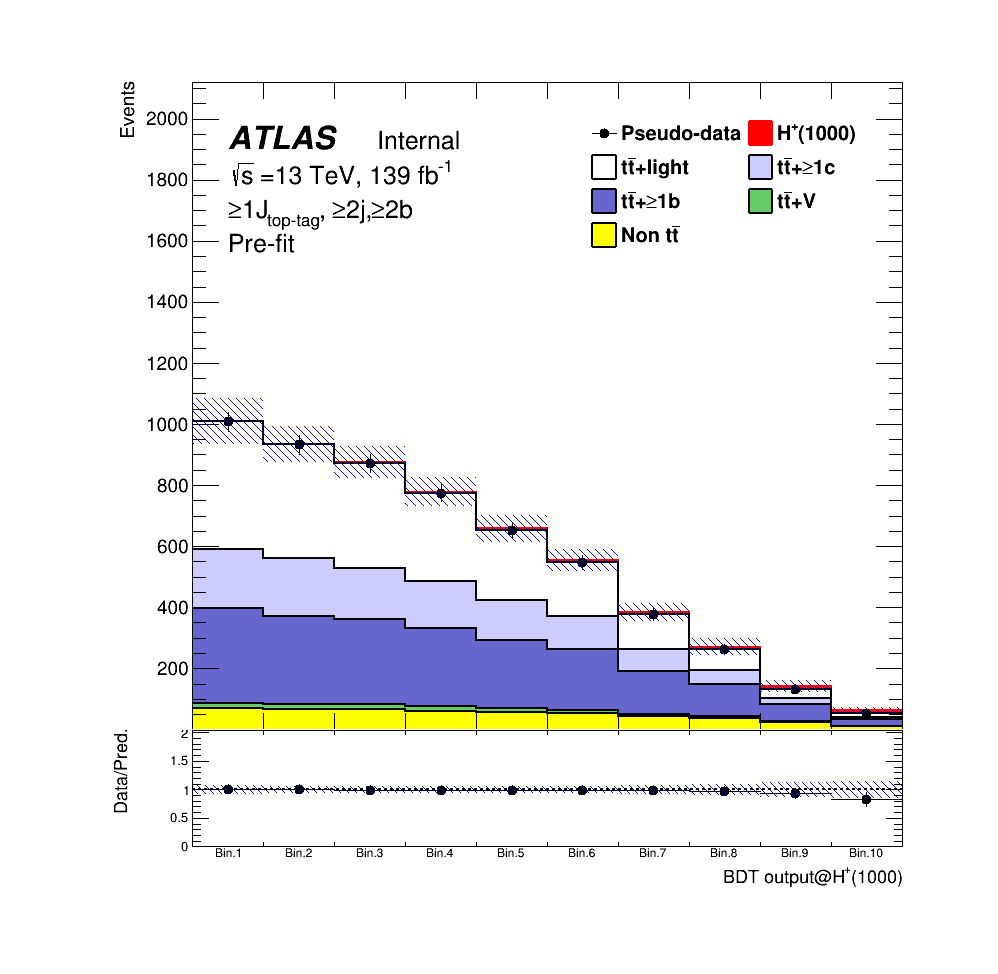
\includegraphics[width=0.45\textwidth]{images/ProfileLHFit/Prefit_Hp1000_asimov_SR.png}
  }
  \subfloat[]{
    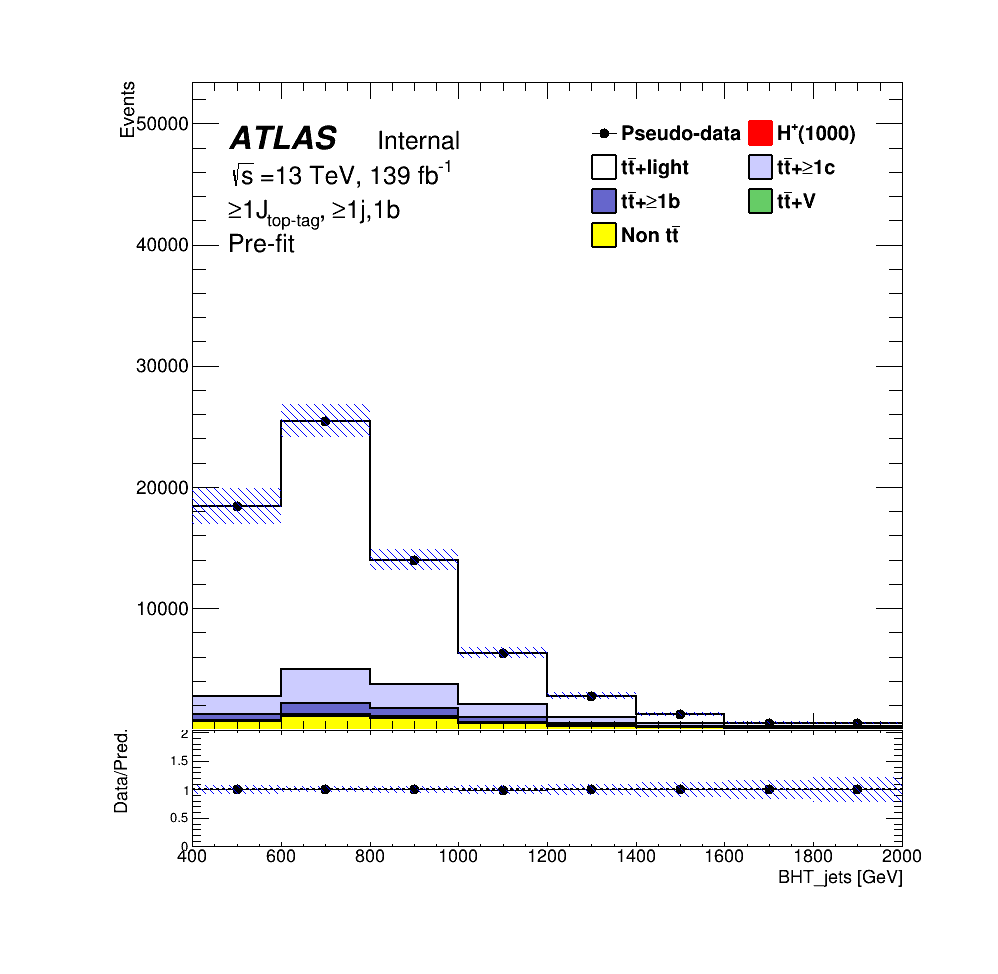
\includegraphics[width=0.45\textwidth]{images/ProfileLHFit/Prefit_Hp1000_asimov_CR.png}
  }
  \caption{Pre-fit plots in the SR (left) and CR (right) for 1000 GeV mass hypothesis of $H^{+}$ signal.}
  \label{fig:Prefit_Hp1000_Asimov}
\end{figure}
\begin{figure}[H]
  \centering
  \subfloat[]{
    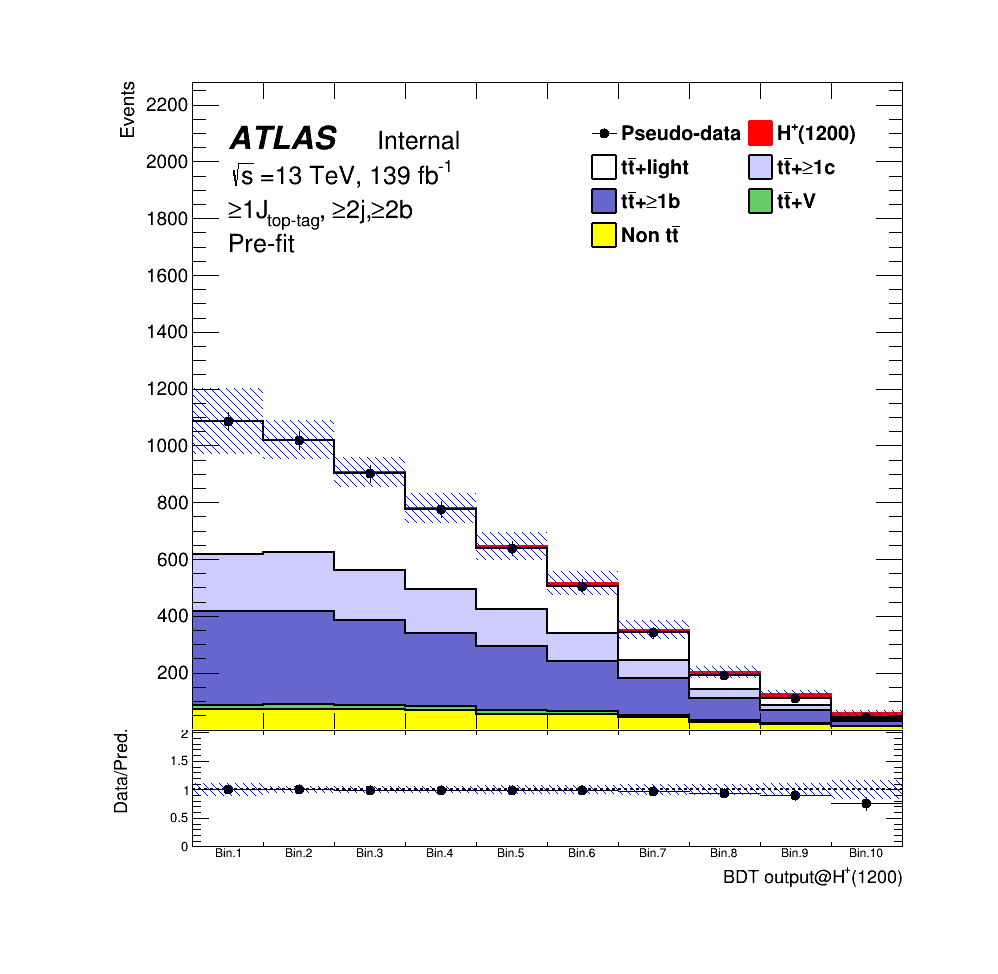
\includegraphics[width=0.45\textwidth]{images/ProfileLHFit/Prefit_Hp1200_asimov_SR.png}
  }
  \subfloat[]{
    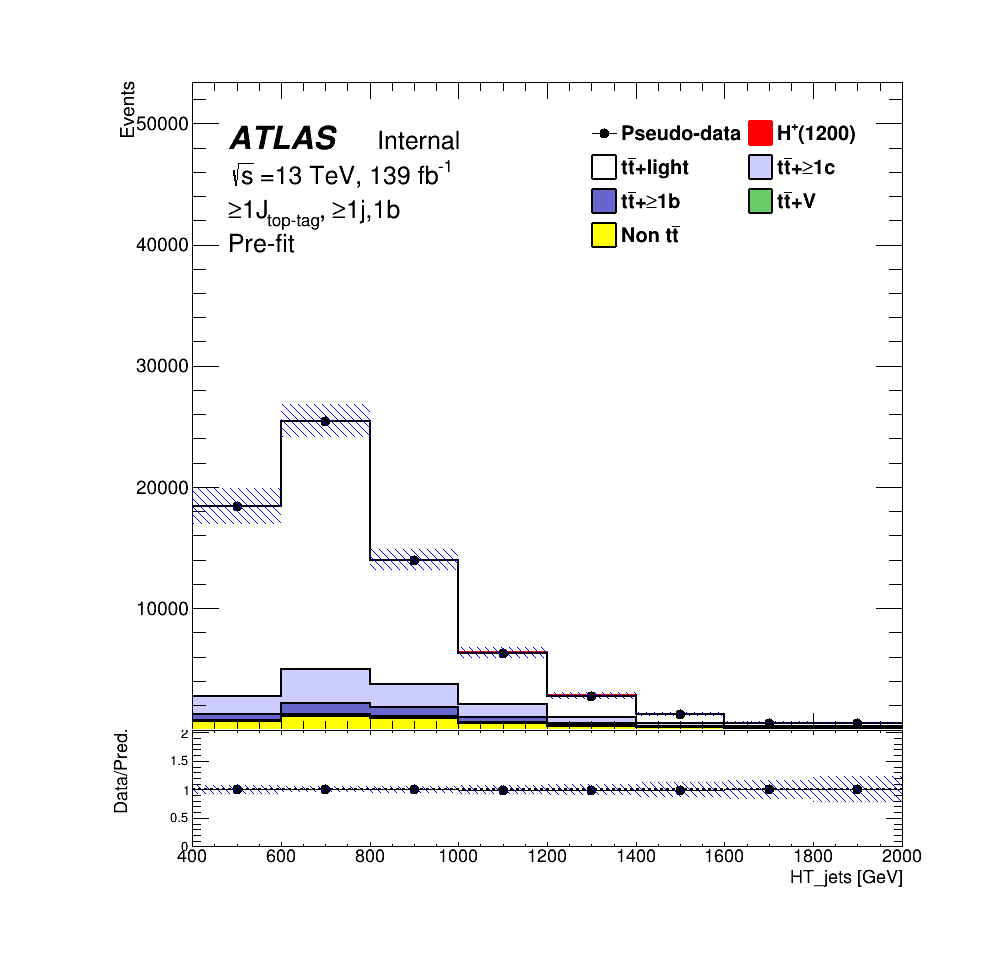
\includegraphics[width=0.45\textwidth]{images/ProfileLHFit/Prefit_Hp1200_asimov_CR.png}
  }
  \caption{Pre-fit plots in the SR (left) and CR (right) for 1200 GeV mass hypothesis of $H^{+}$ signal.}
  \label{fig:Prefit_Hp1200_Asimov}
\end{figure}
\begin{figure}[H]
  \centering
  \subfloat[]{
    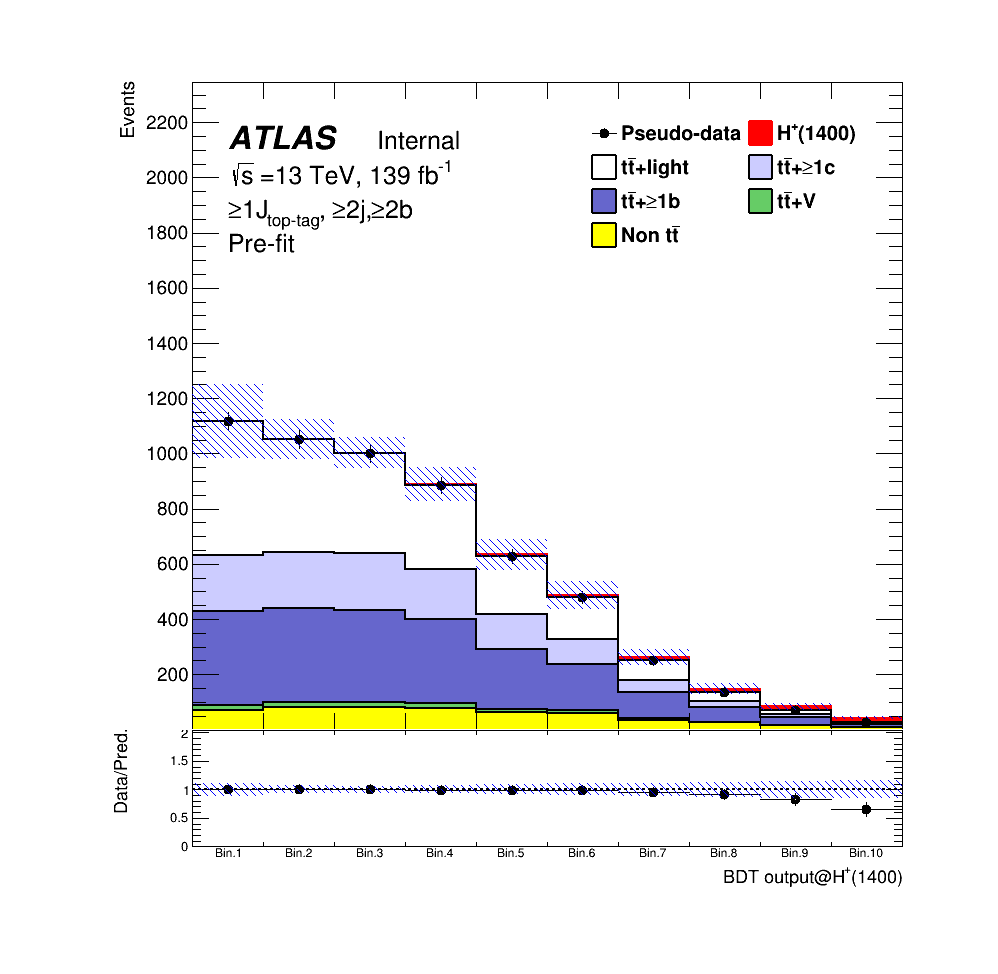
\includegraphics[width=0.45\textwidth]{images/ProfileLHFit/Prefit_Hp1400_asimov_SR.png}
  }
  \subfloat[]{
    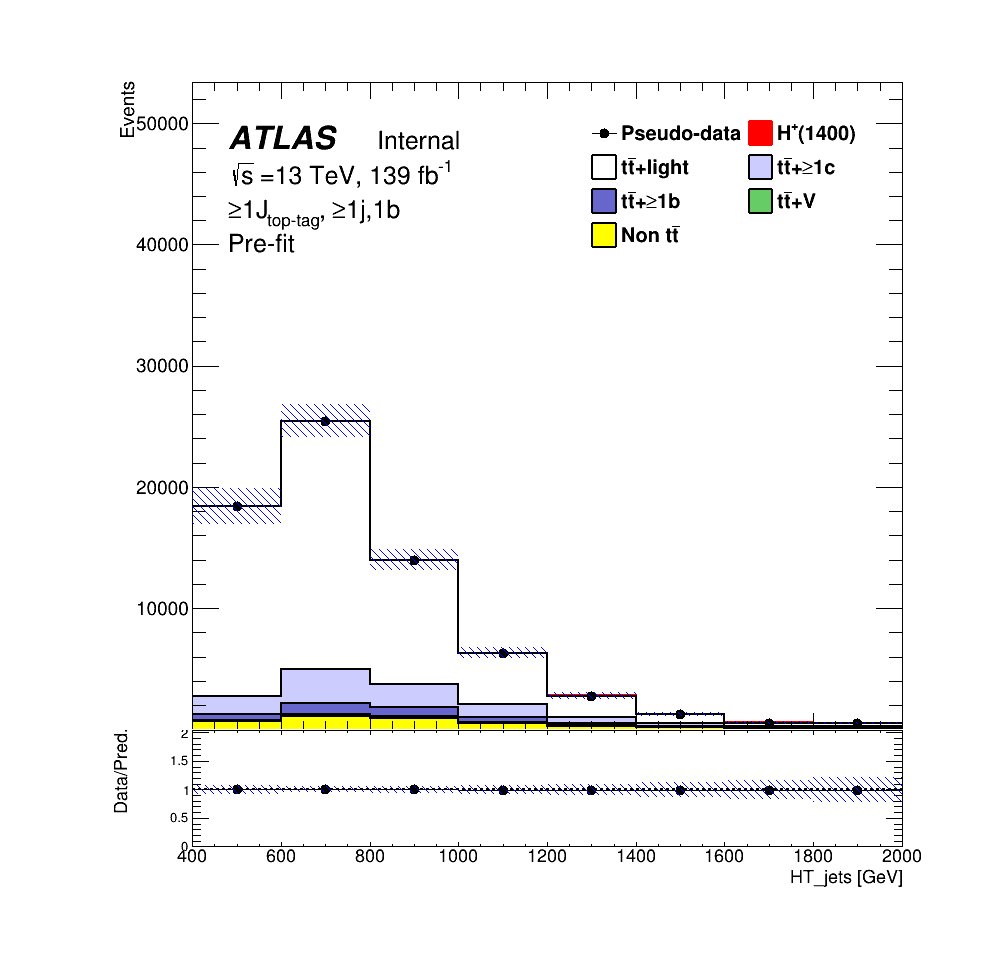
\includegraphics[width=0.45\textwidth]{images/ProfileLHFit/Prefit_Hp1400_asimov_CR.png}
  }
  \caption{Pre-fit plots in the SR (left) and CR (right) for 1400 GeV mass hypothesis of $H^{+}$ signal.}
  \label{fig:Prefit_Hp1400_Asimov}
\end{figure}
\begin{figure}[H]
  \centering
  \subfloat[]{
    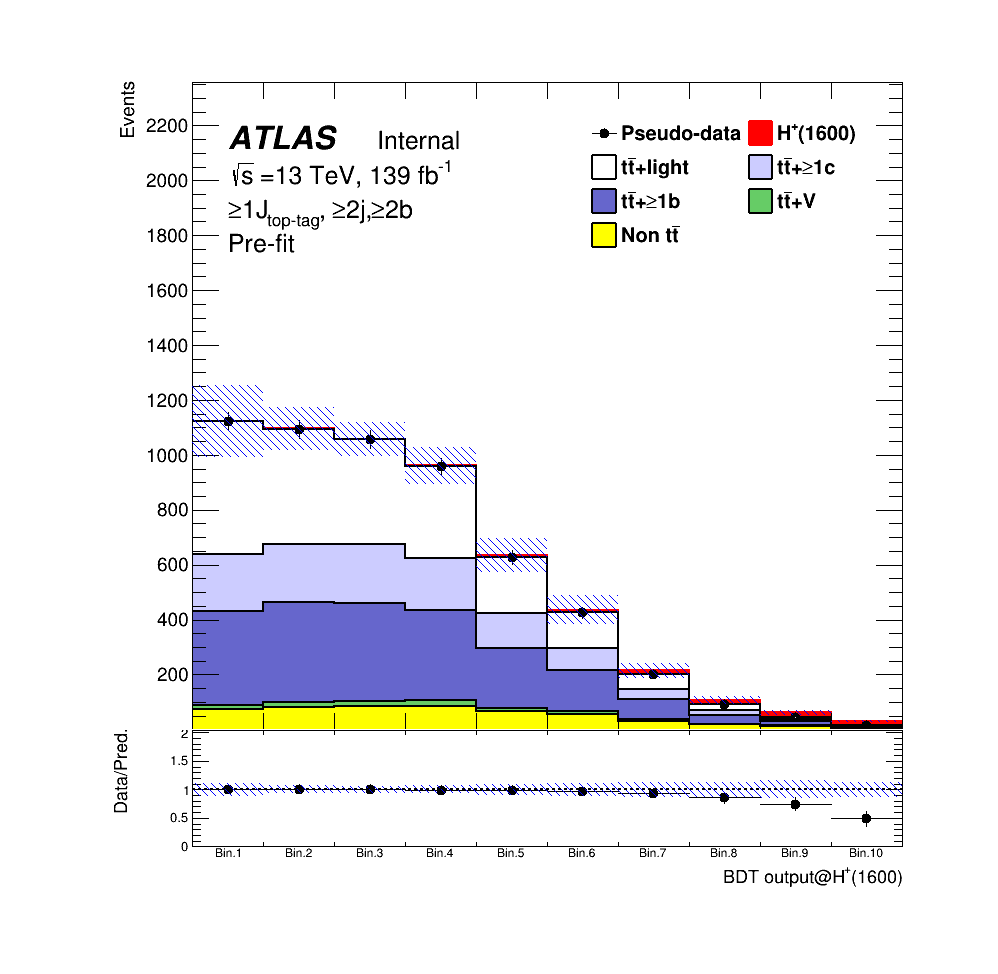
\includegraphics[width=0.45\textwidth]{images/ProfileLHFit/Prefit_Hp1600_asimov_SR.png}
  }
  \subfloat[]{
    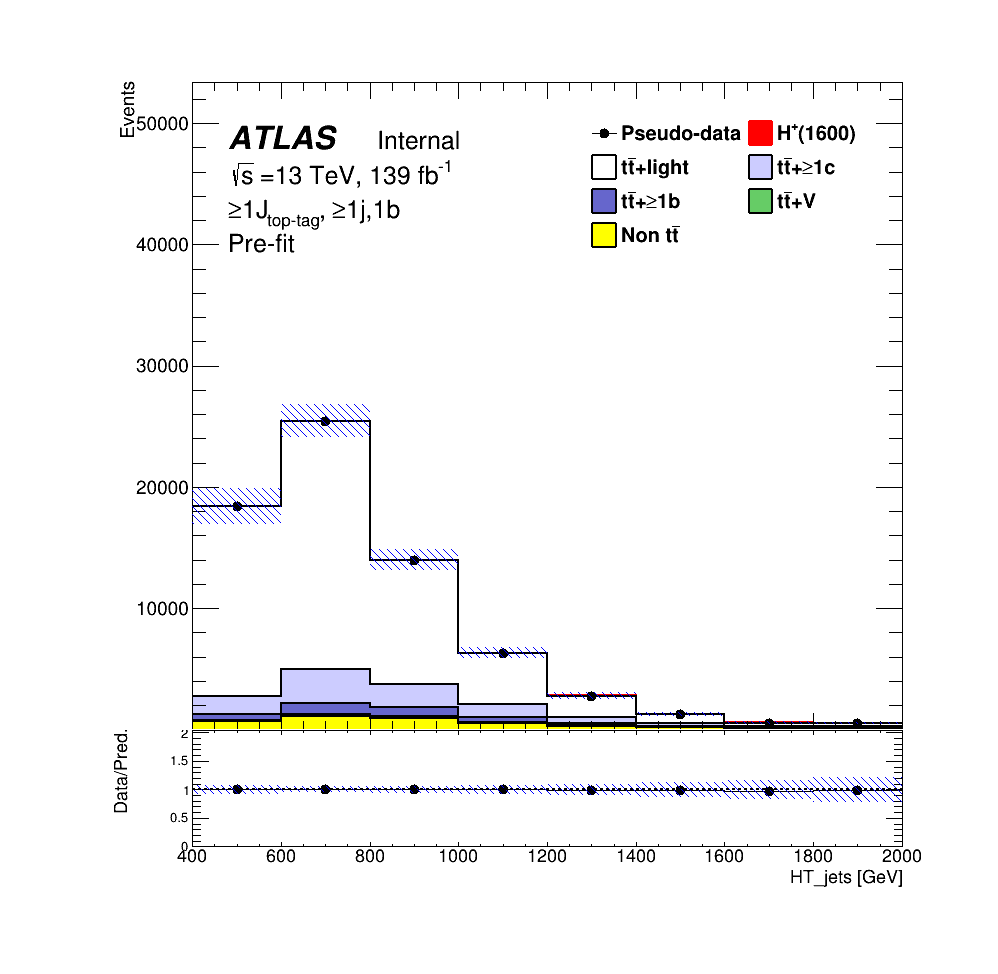
\includegraphics[width=0.45\textwidth]{images/ProfileLHFit/Prefit_Hp1600_asimov_CR.png}
  }
  \caption{Pre-fit plots in the SR (left) and CR (right) for 1600 GeV mass hypothesis of $H^{+}$ signal.}
  \label{fig:Prefit_Hp1600_Asimov}
\end{figure}
\begin{figure}[H]
  \centering
  \subfloat[]{
    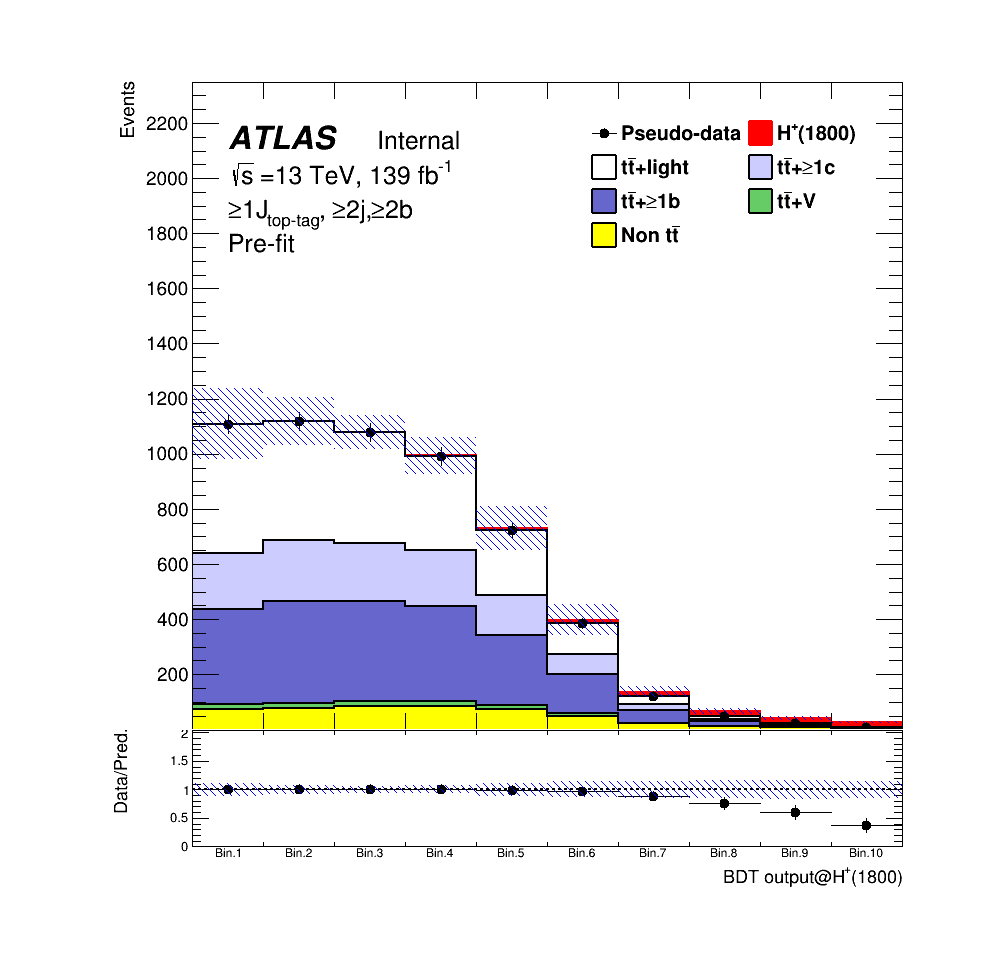
\includegraphics[width=0.45\textwidth]{images/ProfileLHFit/Prefit_Hp1800_asimov_SR.png}
  }
  \subfloat[]{
    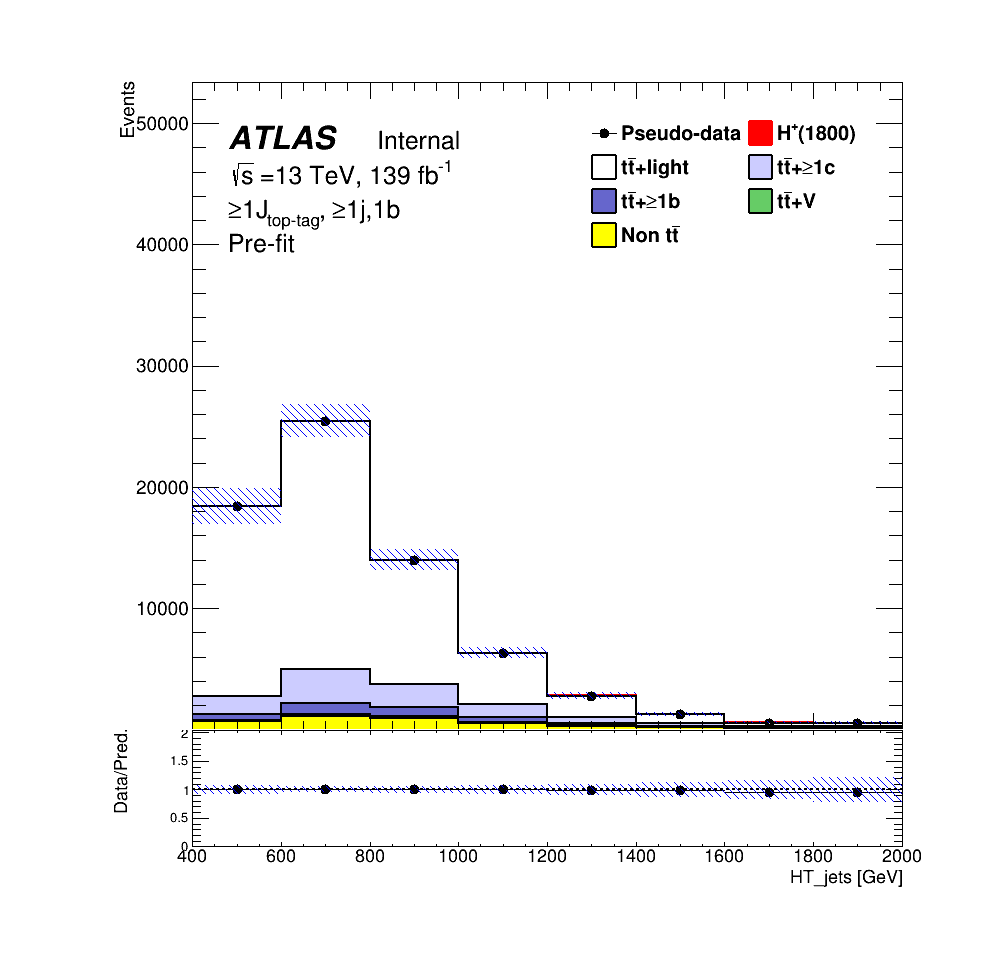
\includegraphics[width=0.45\textwidth]{images/ProfileLHFit/Prefit_Hp1800_asimov_CR.png}
  }
  \caption{Pre-fit plots in the SR (left) and CR (right) for 1800 GeV mass hypothesis of $H^{+}$ signal.}
  \label{fig:Prefit_Hp1800_Asimov}
\end{figure}
\begin{figure}[H]
  \centering
  \subfloat[]{
    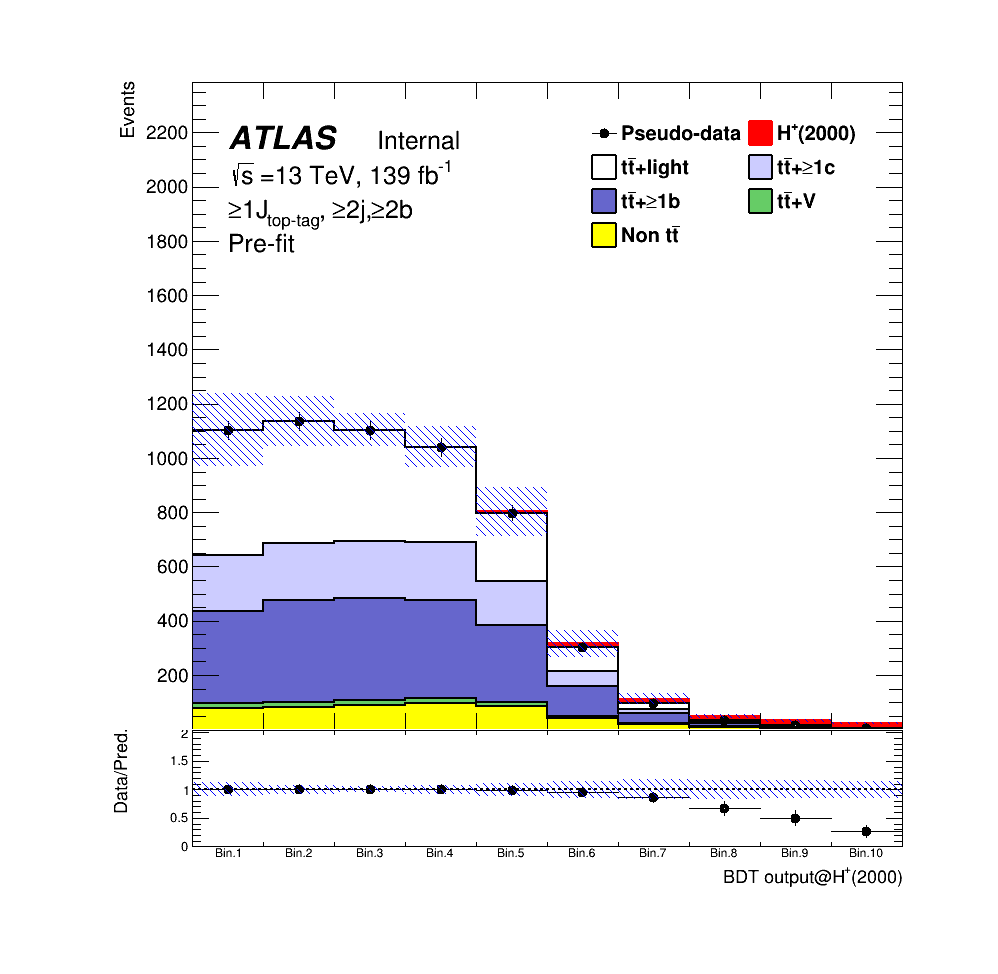
\includegraphics[width=0.45\textwidth]{images/ProfileLHFit/Prefit_Hp2000_asimov_SR.png}
  }
  \subfloat[]{
    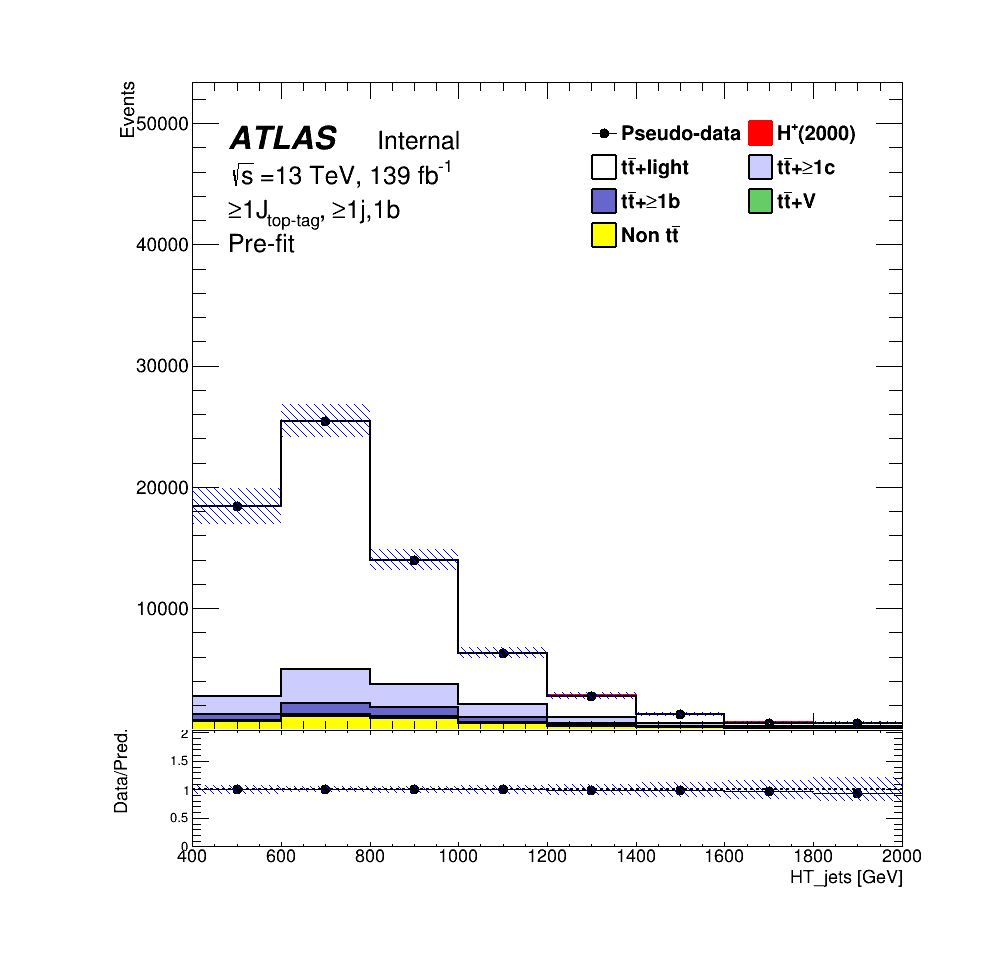
\includegraphics[width=0.45\textwidth]{images/ProfileLHFit/Prefit_Hp2000_asimov_CR.png}
  }
  \caption{Pre-fit plots in the SR (left) and CR (right) for 2000 GeV mass hypothesis of $H^{+}$ signal.}
  \label{fig:Prefit_Hp2000_Asimov}
\end{figure}
\begin{figure}[H]
  \centering
  \subfloat[]{
    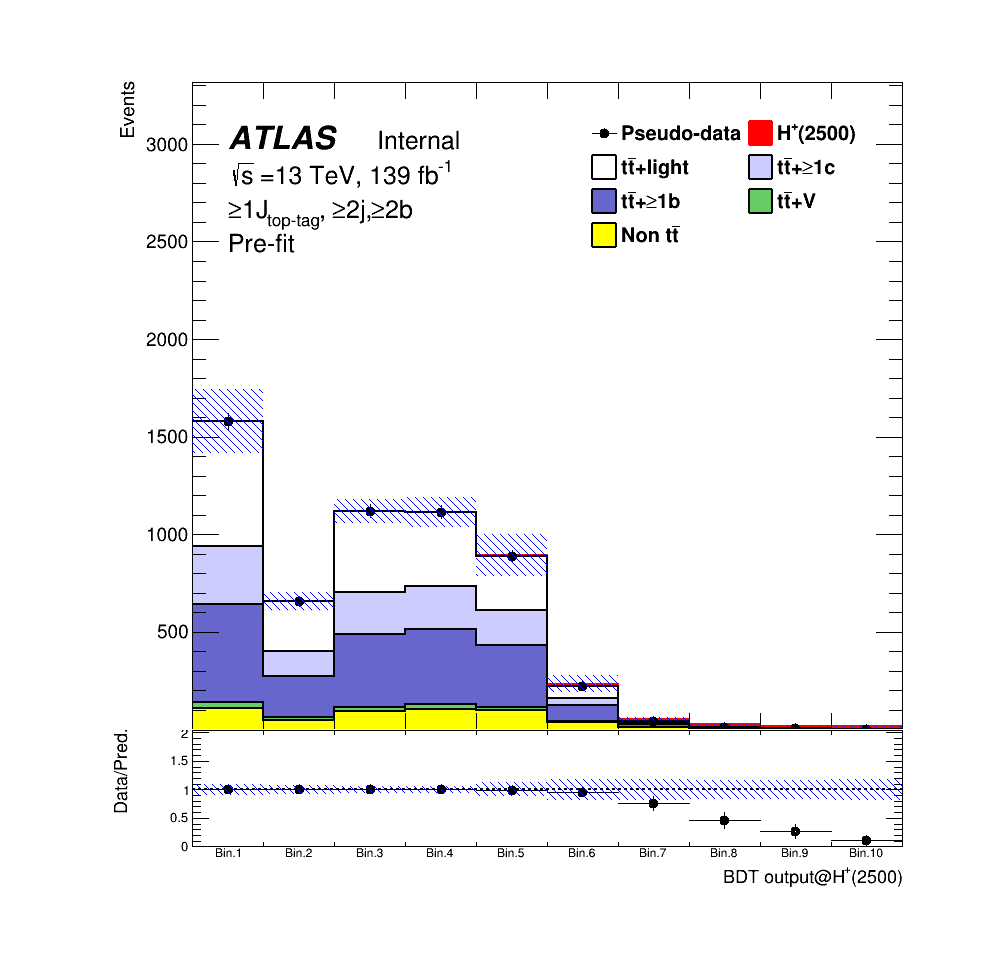
\includegraphics[width=0.45\textwidth]{images/ProfileLHFit/Prefit_Hp2500_asimov_SR.png}
  }
  \subfloat[]{
    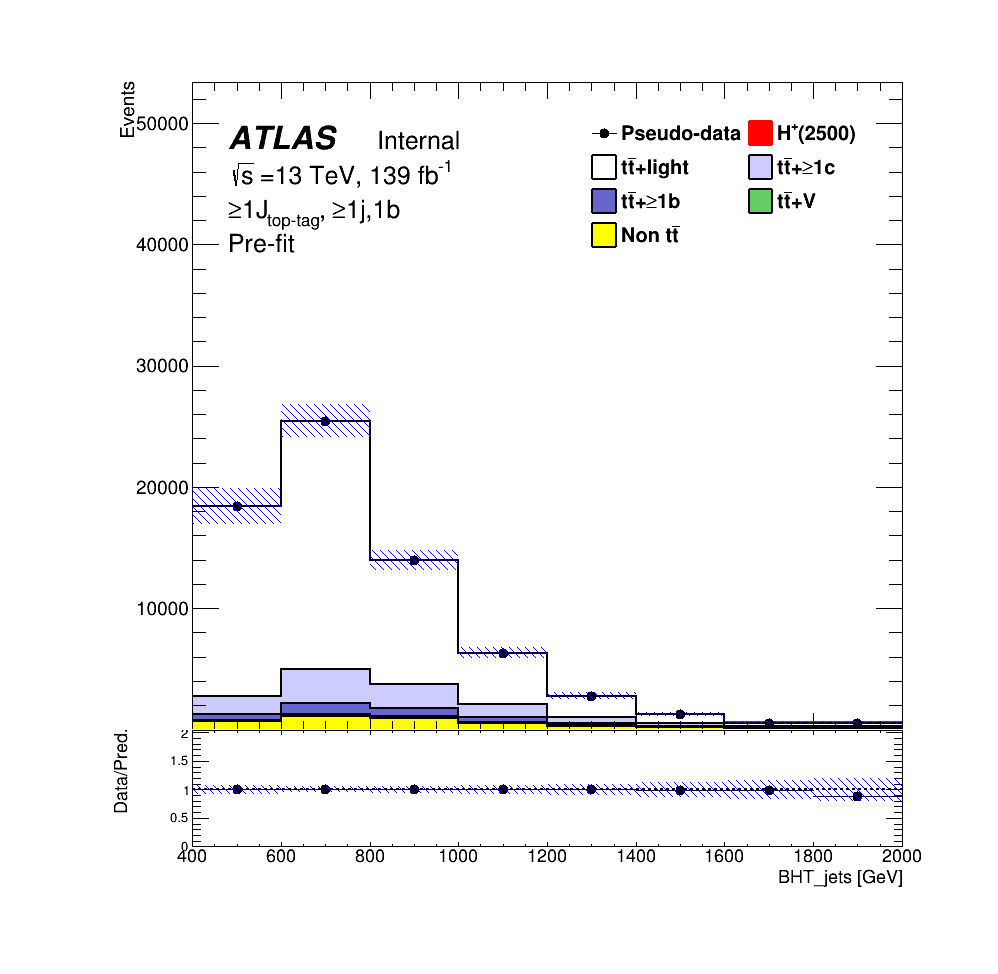
\includegraphics[width=0.45\textwidth]{images/ProfileLHFit/Prefit_Hp2500_asimov_CR.png}
  }
  \caption{Pre-fit plots in the SR (left) and CR (right) for 2500 GeV mass hypothesis of $H^{+}$ signal.}
  \label{fig:Prefit_Hp2500_Asimov}
\end{figure}
\begin{figure}[H]
  \centering
  \subfloat[]{
    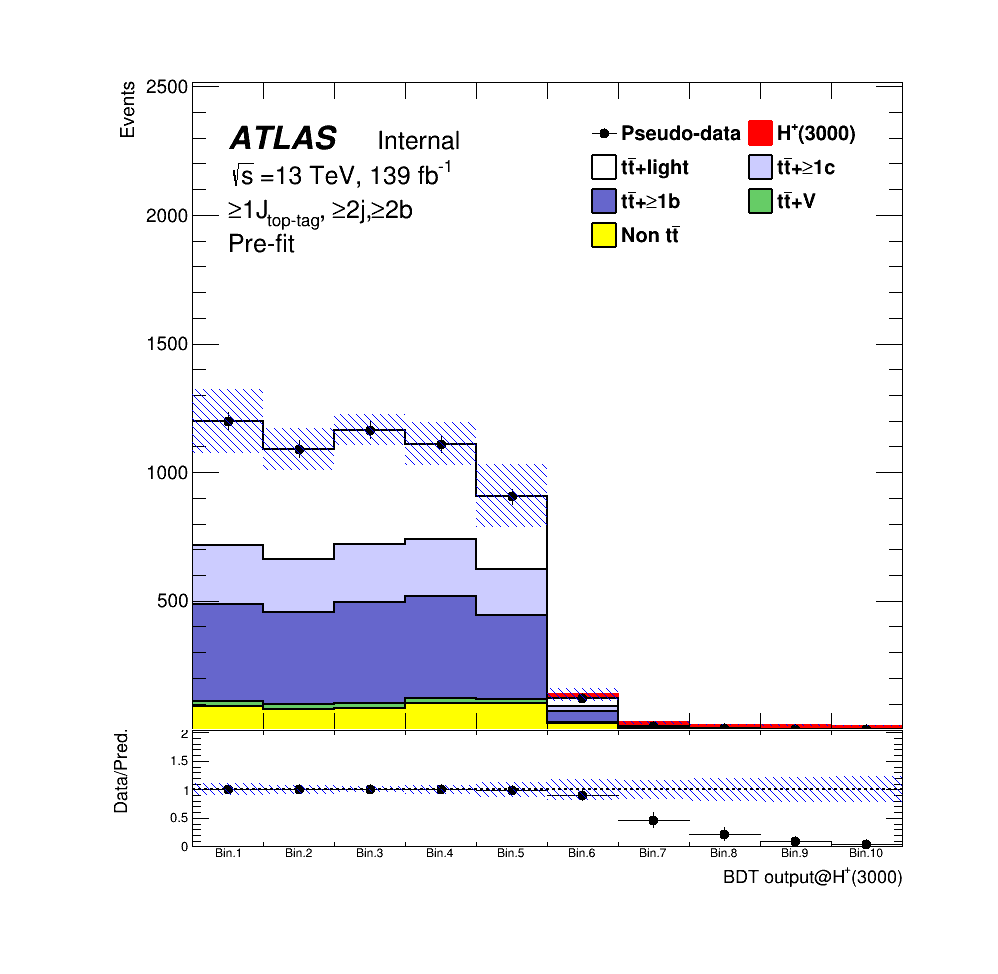
\includegraphics[width=0.45\textwidth]{images/ProfileLHFit/Prefit_Hp3000_asimov_SR.png}
  }
  \subfloat[]{
    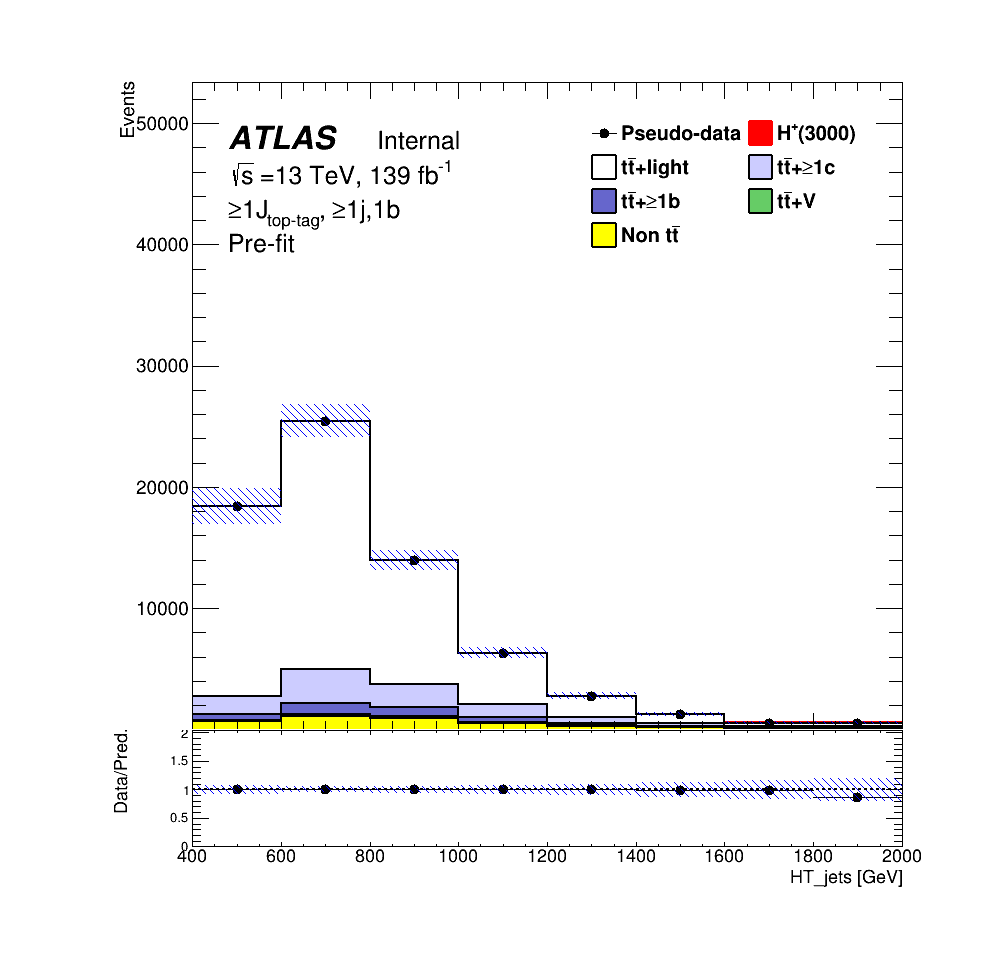
\includegraphics[width=0.45\textwidth]{images/ProfileLHFit/Prefit_Hp3000_asimov_CR.png}
  }
  \caption{Pre-fit plots in the SR (left) and CR (right) for 3000 GeV mass hypothesis of $H^{+}$ signal.}
  \label{fig:Prefit_Hp3000_Asimov}
\end{figure}

\begin{figure}[H]
  \centering
  \subfloat[]{
    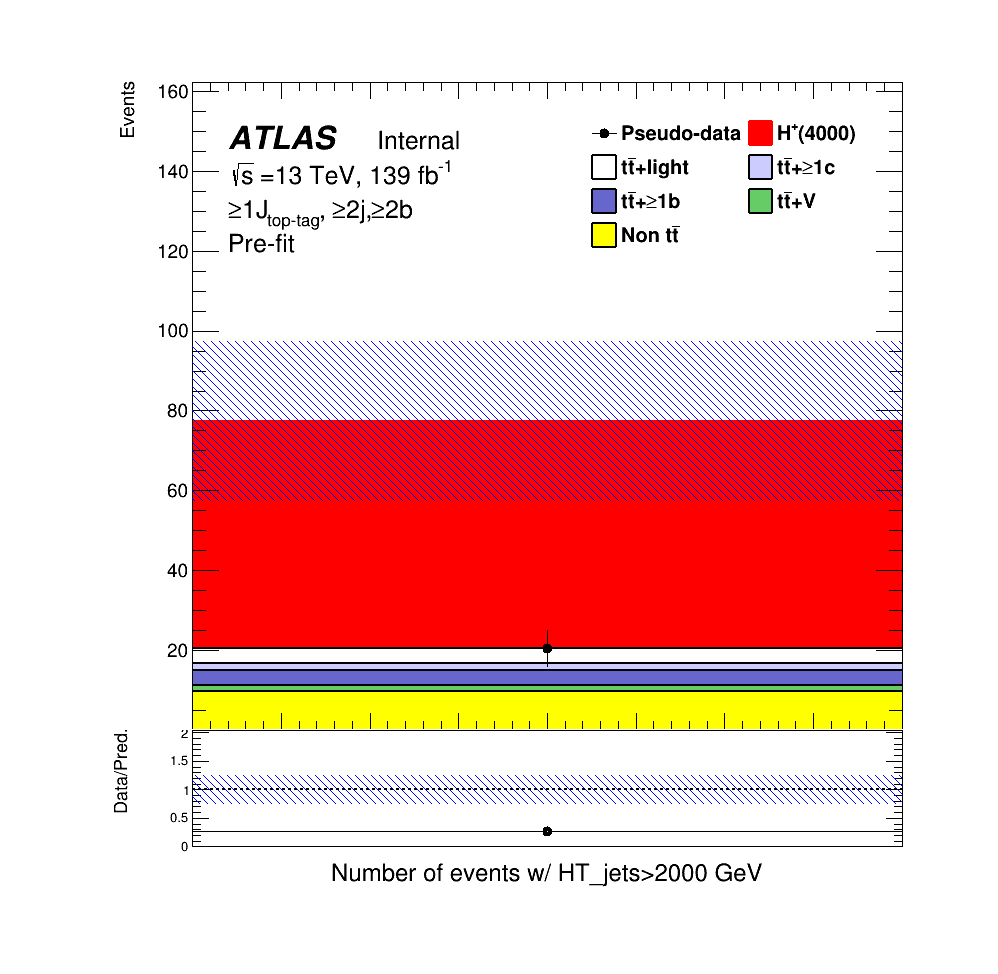
\includegraphics[width=0.45\textwidth]{images/ProfileLHFit/Prefit_Hp4000_asimov_SR.png}
    \label{fig:Prefit_Hp4000_Asimov_SR}
  }\par
  \subfloat[]{
    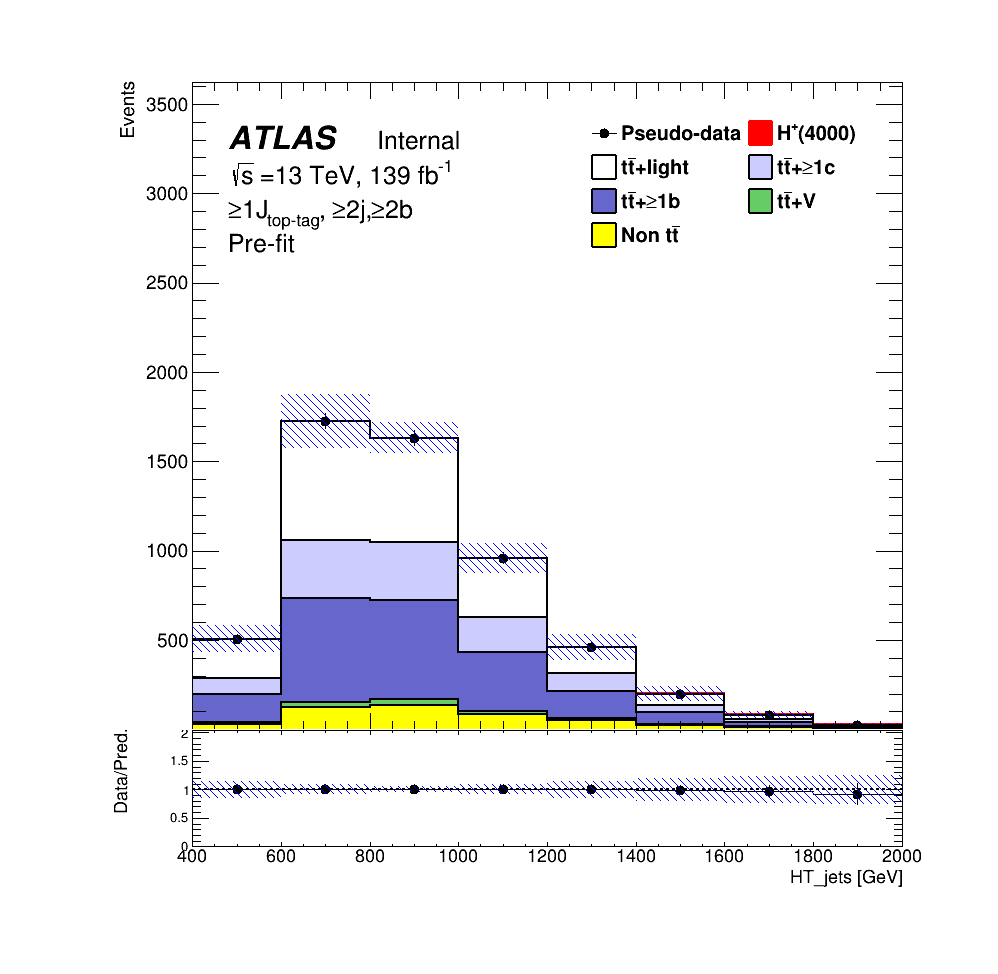
\includegraphics[width=0.45\textwidth]{images/ProfileLHFit/Prefit_Hp4000_asimov_CR1.png}
    \label{fig:Prefit_Hp4000_Asimov_CR1}
  }
  \subfloat[]{
    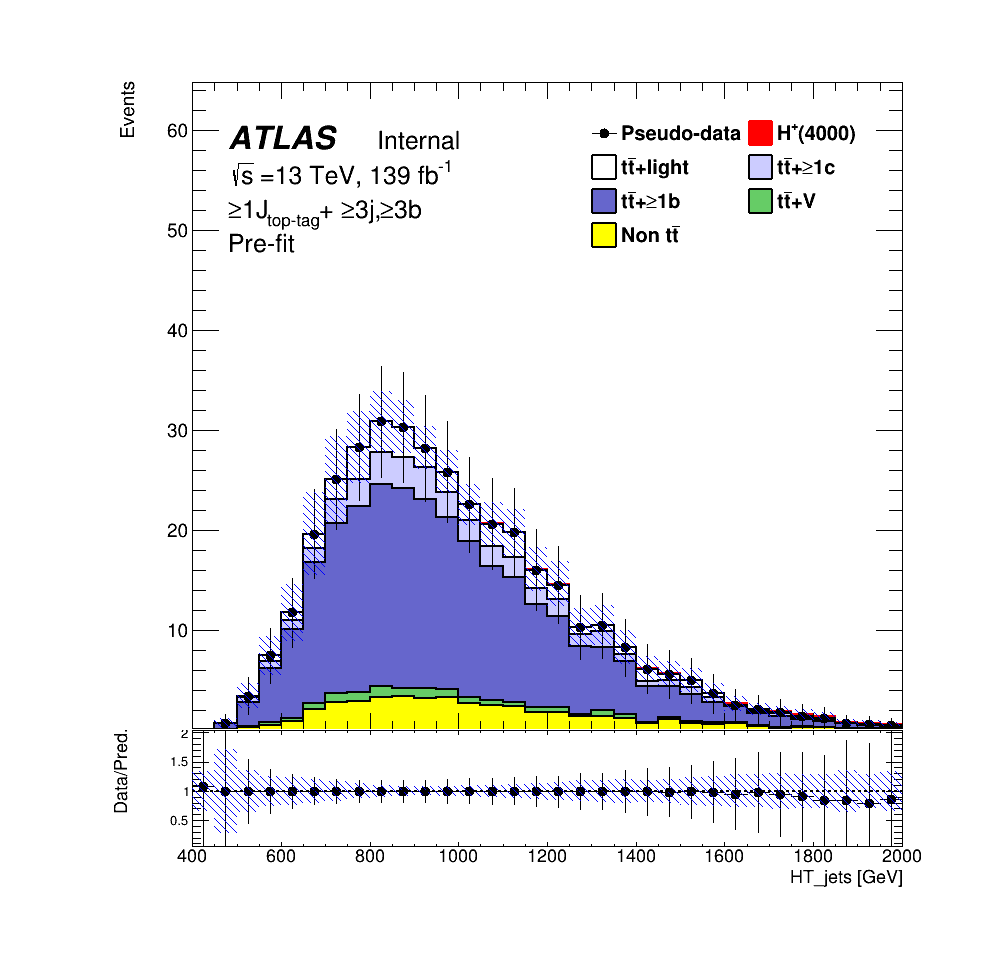
\includegraphics[width=0.45\textwidth]{images/ProfileLHFit/Prefit_Hp4000_asimov_CR2.png}
    \label{fig:Prefit_Hp4000_Asimov_CR2}
  }
  \caption{Pre-fit plots in the SR (top), CR1 (bottom-left), and CR2 (bottom-right) for 4000 GeV mass hypothesis of $H^{+}$ signal.}
  \label{fig:Prefit_Hp4000_Asimov}
\end{figure}

\begin{figure}[H]
  \centering
  \subfloat[]{
    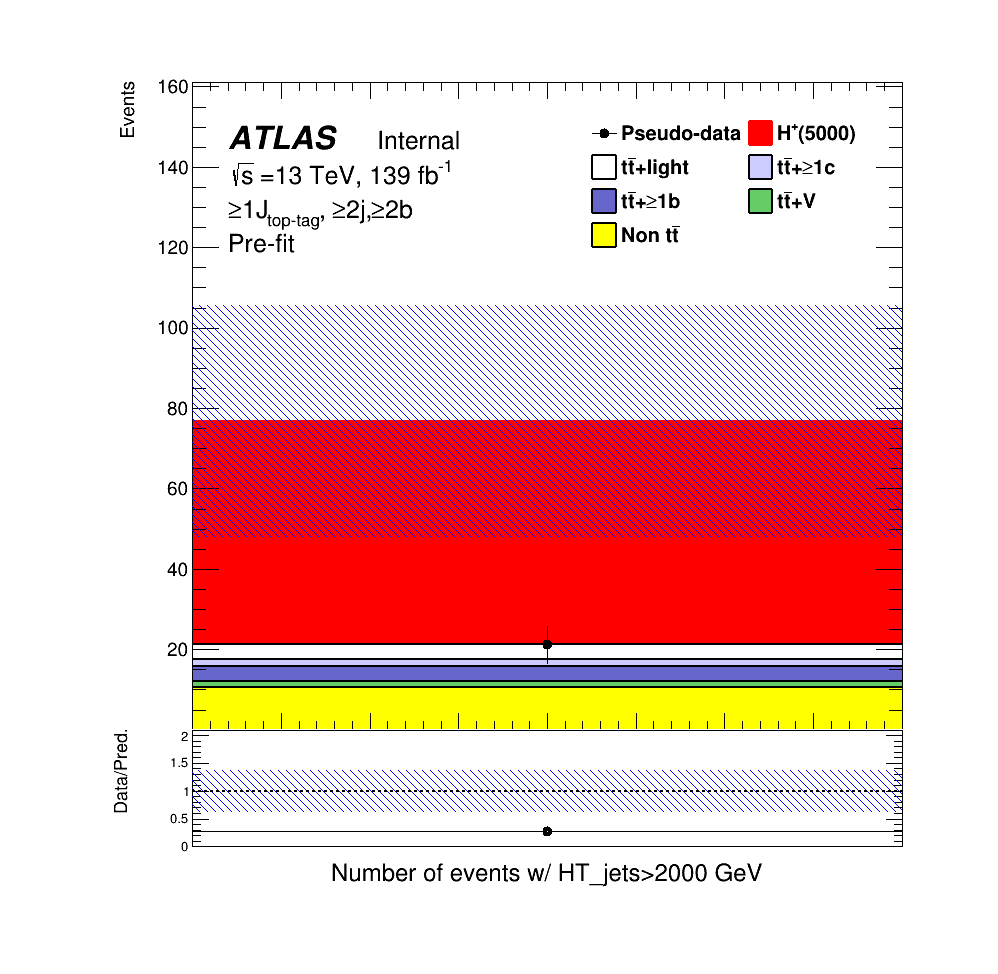
\includegraphics[width=0.45\textwidth]{images/ProfileLHFit/Prefit_Hp5000_asimov_SR.png}
  }\par
  \subfloat[]{
    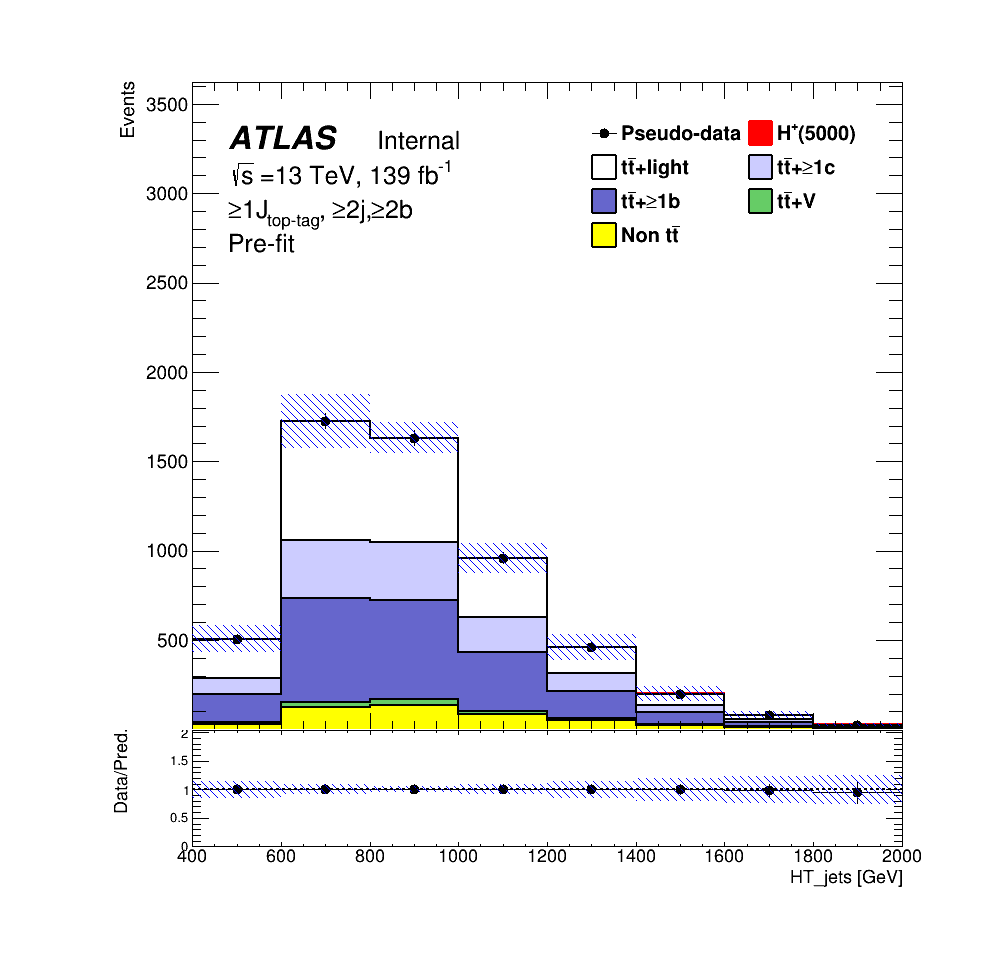
\includegraphics[width=0.45\textwidth]{images/ProfileLHFit/Prefit_Hp5000_asimov_CR1.png}
  }
  \subfloat[]{
    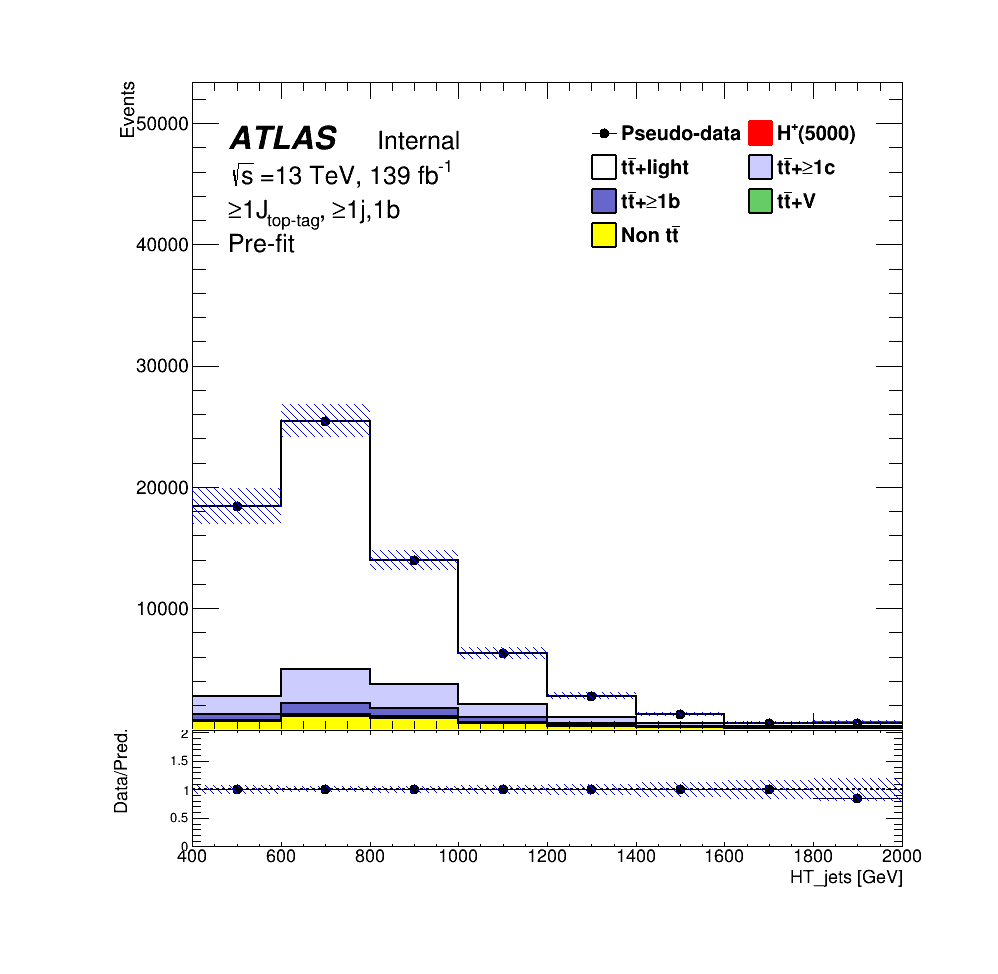
\includegraphics[width=0.45\textwidth]{images/ProfileLHFit/Prefit_Hp5000_asimov_CR2.png}
  }
  \caption{Pre-fit plots in the SR (top), CR1 (bottom-left), and CR2 (bottom-right) for 5000 GeV mass hypothesis of $H^{+}$ signal.}
  \label{fig:Prefit_Hp5000_Asimov}
\end{figure}

% --- Pre-fit plots for W'-LH
\begin{figure}[H]
  \centering
  \subfloat[]{
    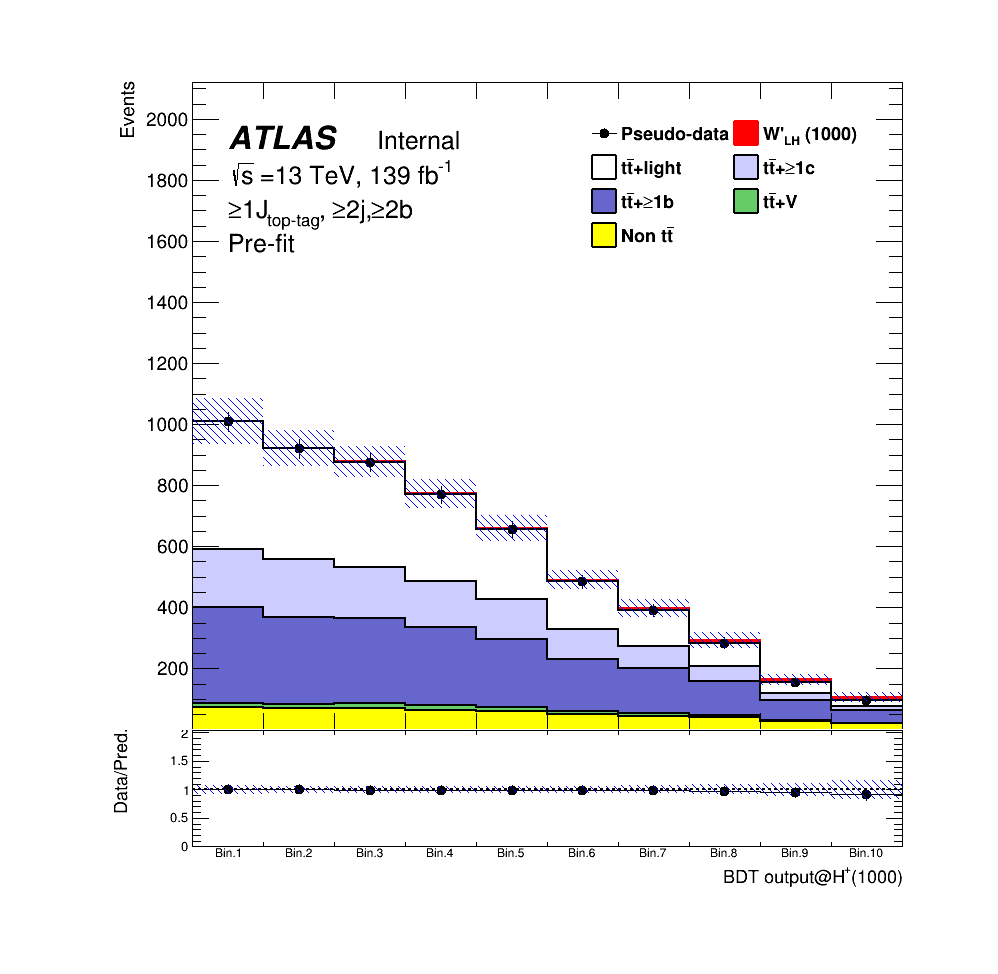
\includegraphics[width=0.45\textwidth]{images/ProfileLHFit/Prefit_Wp1000-LH_asimov_SR.png}
  }
  \subfloat[]{
    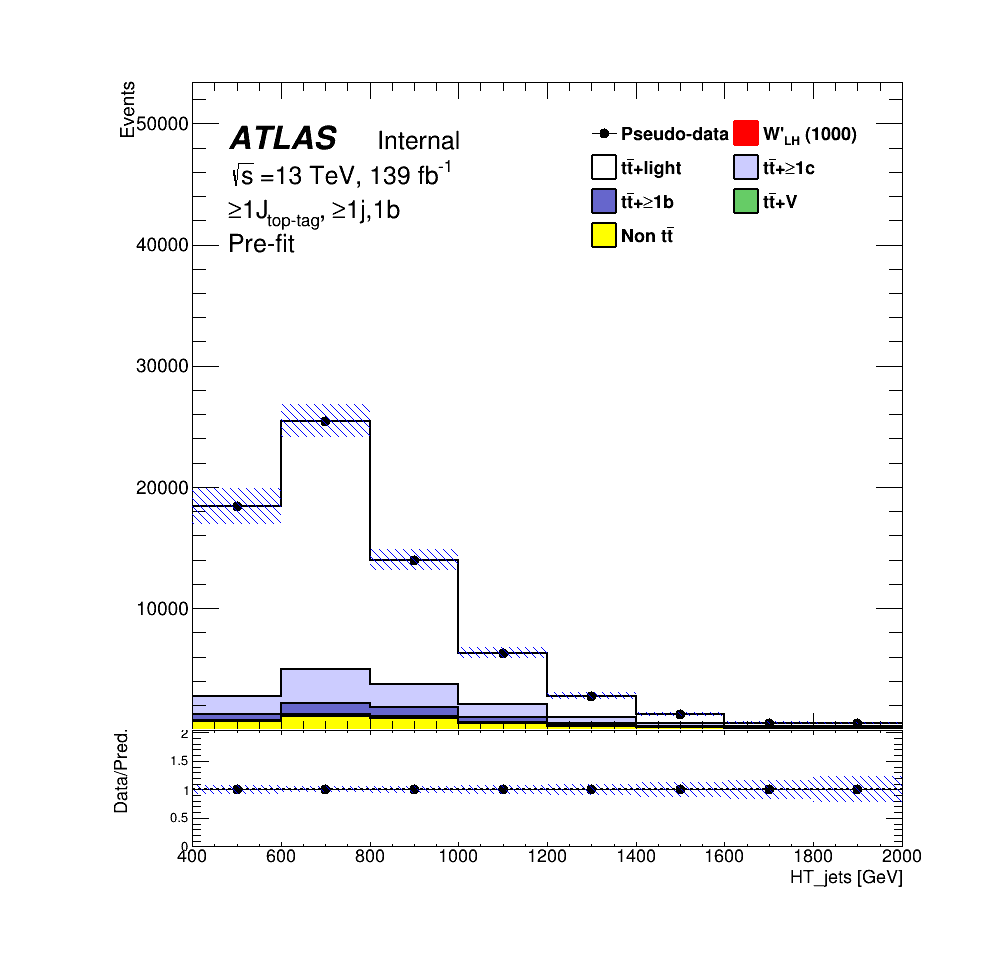
\includegraphics[width=0.45\textwidth]{images/ProfileLHFit/Prefit_Wp1000-LH_asimov_CR.png}
  }
  \caption{Pre-fit plots in the SR (left) and CR (right) for 1000 GeV mass hypothesis of $W'_{\text{L}}$ signal.}
  \label{fig:Prefit_WpLH1000_Asimov}
\end{figure}
\begin{figure}[H]
  \centering
  \subfloat[]{
    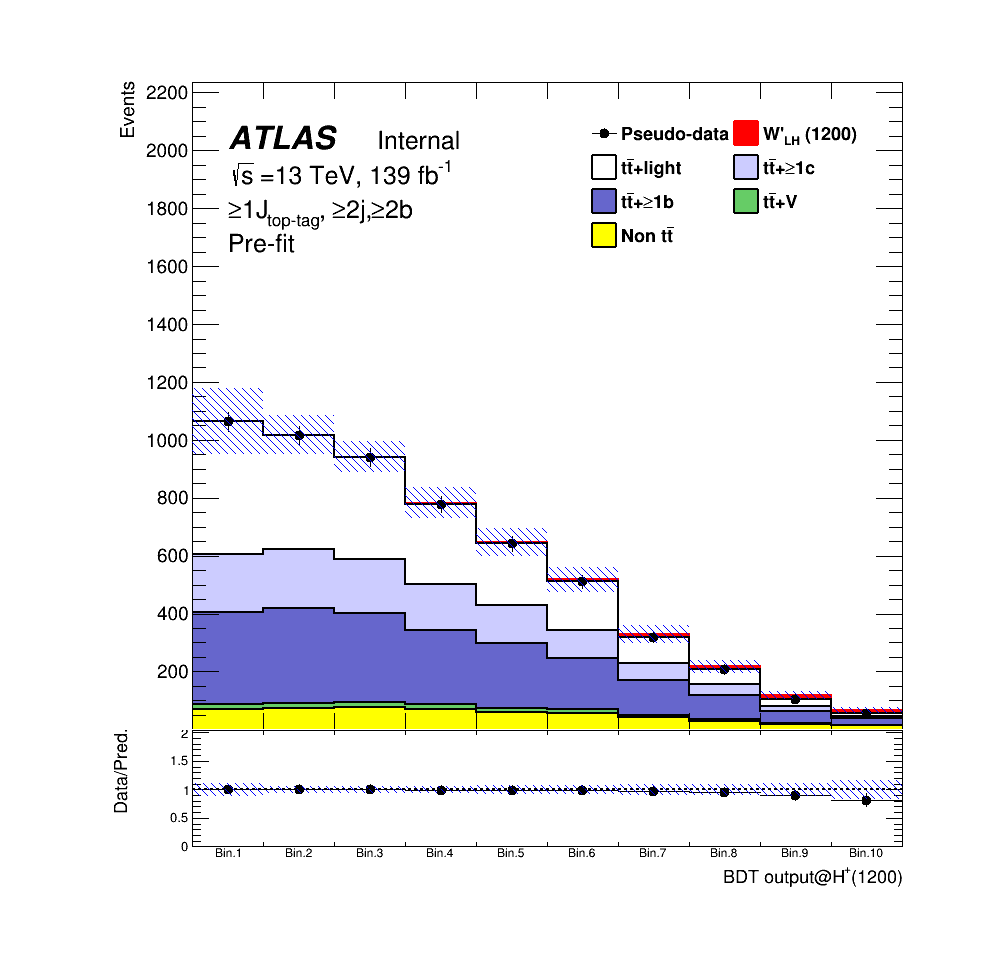
\includegraphics[width=0.45\textwidth]{images/ProfileLHFit/Prefit_Wp1200-LH_asimov_SR.png}
  }
  \subfloat[]{
    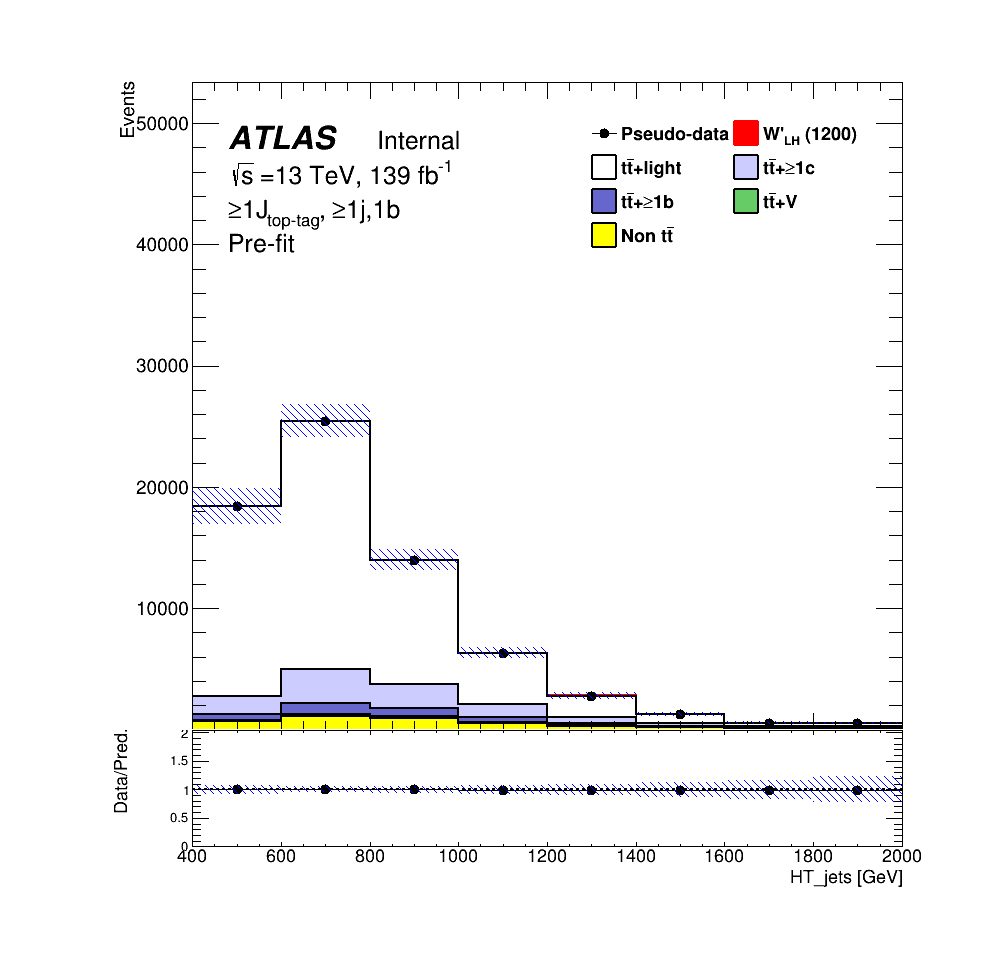
\includegraphics[width=0.45\textwidth]{images/ProfileLHFit/Prefit_Wp1200-LH_asimov_CR.png}
  }
  \caption{Pre-fit plots in the SR (left) and CR (right) for 1200 GeV mass hypothesis of $W'_{\text{L}}$ signal.}
  \label{fig:Prefit_WpLH1200_Asimov}
\end{figure}
\begin{figure}[H]
  \centering
  \subfloat[]{
    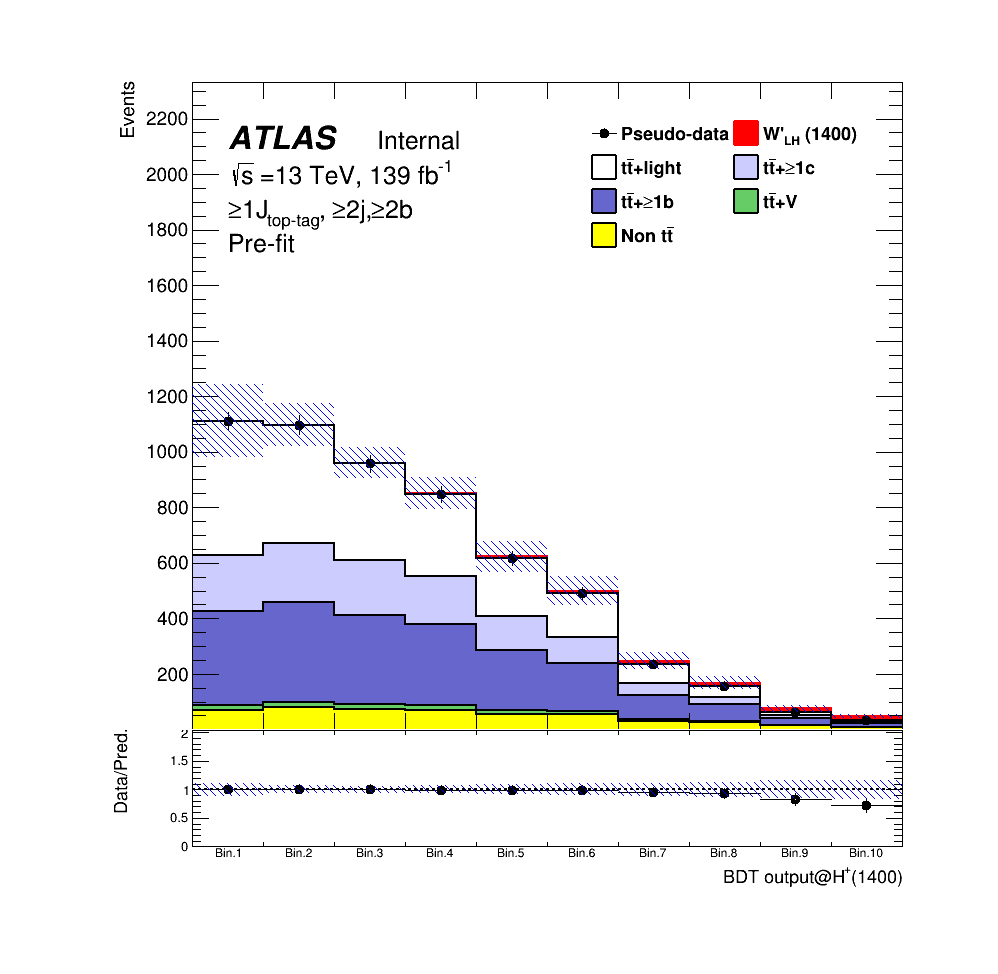
\includegraphics[width=0.45\textwidth]{images/ProfileLHFit/Prefit_Wp1400-LH_asimov_SR.png}
  }
  \subfloat[]{
    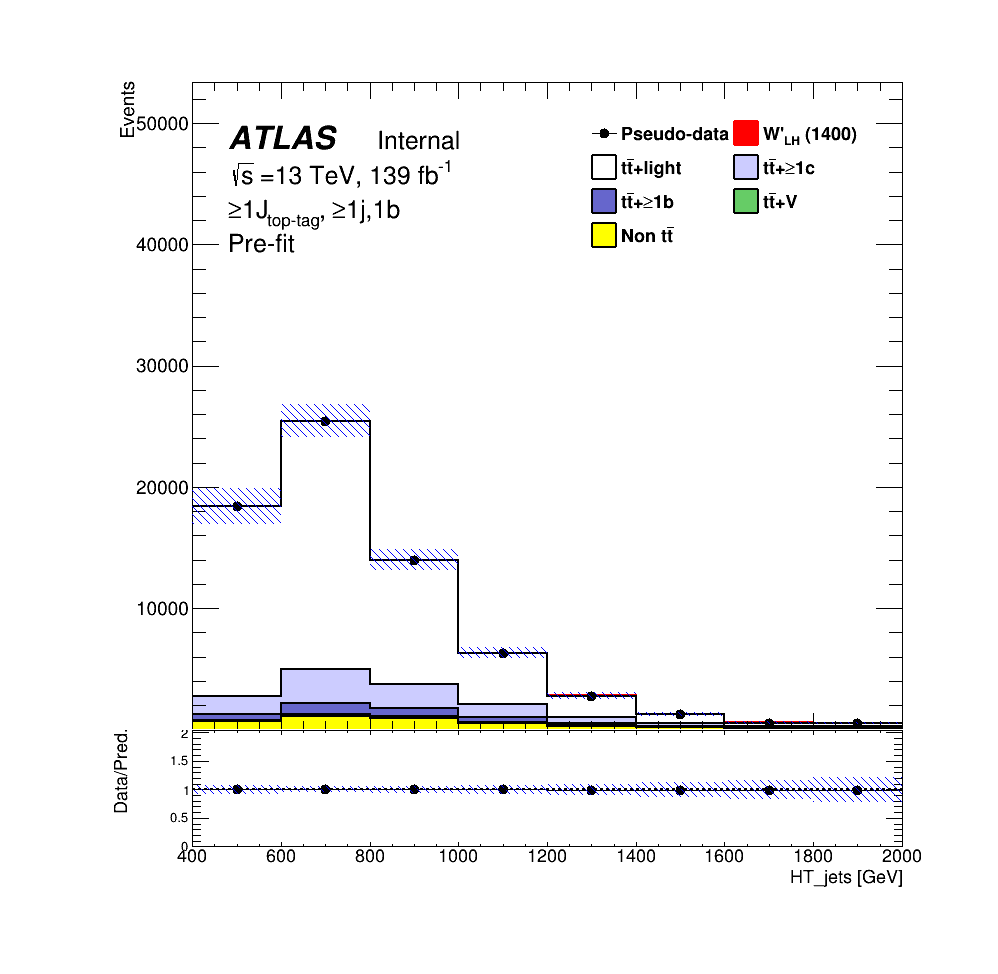
\includegraphics[width=0.45\textwidth]{images/ProfileLHFit/Prefit_Wp1400-LH_asimov_CR.png}
  }
  \caption{Pre-fit plots in the SR (left) and CR (right) for 1400 GeV mass hypothesis of $W'_{\text{L}}$ signal.}
  \label{fig:Prefit_WpLH1400_Asimov}
\end{figure}
\begin{figure}[H]
  \centering
  \subfloat[]{
    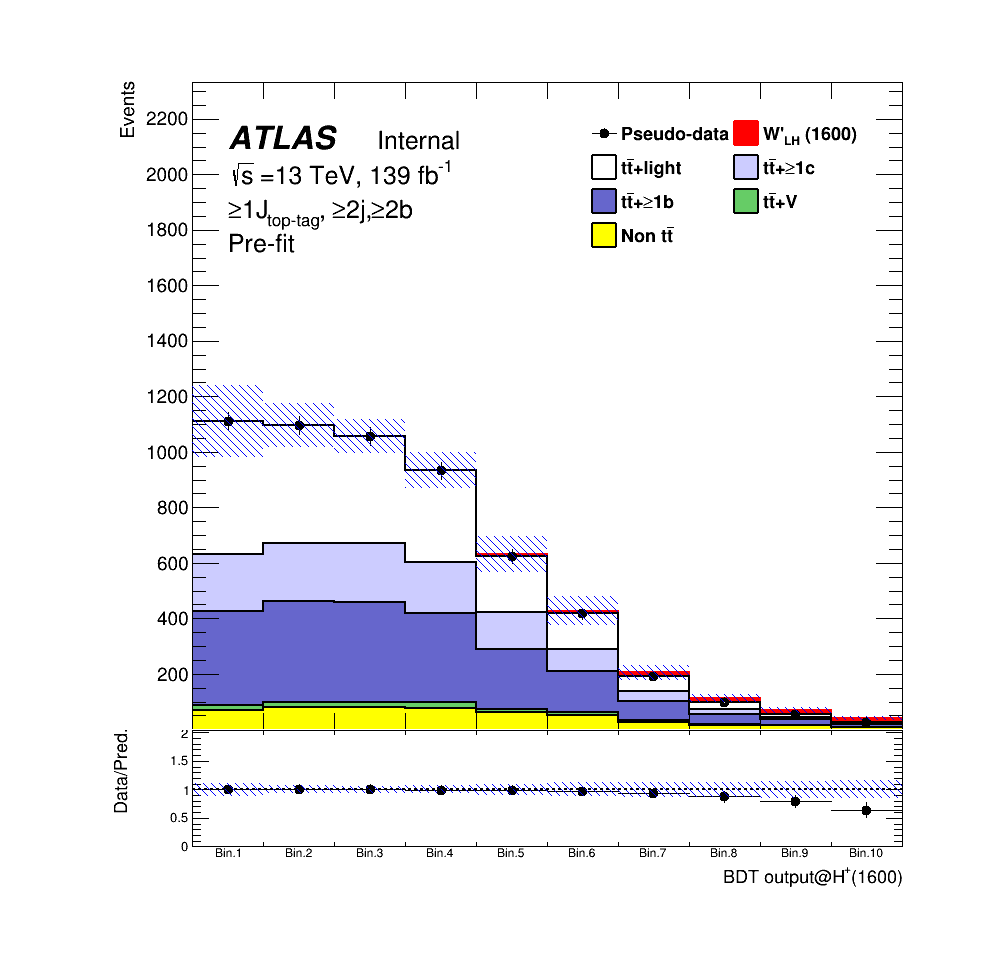
\includegraphics[width=0.45\textwidth]{images/ProfileLHFit/Prefit_Wp1600-LH_asimov_SR.png}
  }
  \subfloat[]{
    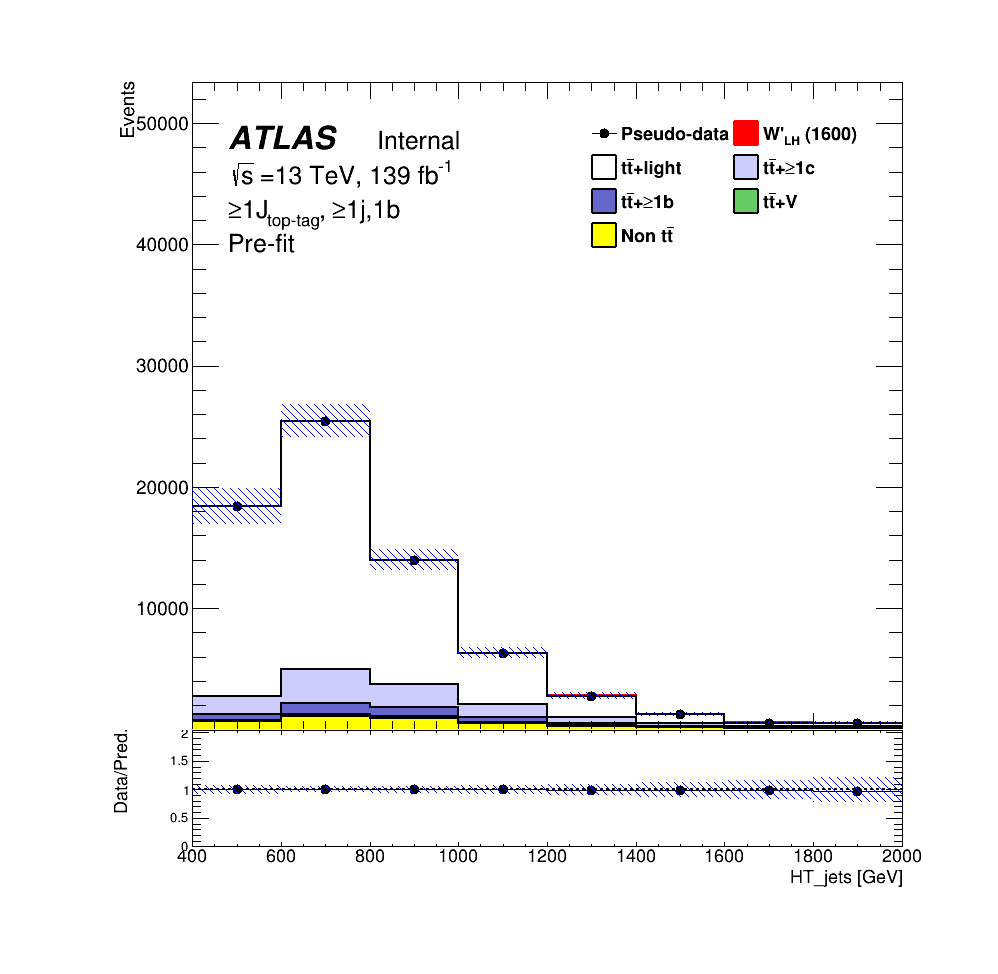
\includegraphics[width=0.45\textwidth]{images/ProfileLHFit/Prefit_Wp1600-LH_asimov_CR.png}
  }
  \caption{Pre-fit plots in the SR (left) and CR (right) for 1600 GeV mass hypothesis of $W'_{\text{L}}$ signal.}
  \label{fig:Prefit_WpLH1600_Asimov}
\end{figure}
\begin{figure}[H]
  \centering
  \subfloat[]{
    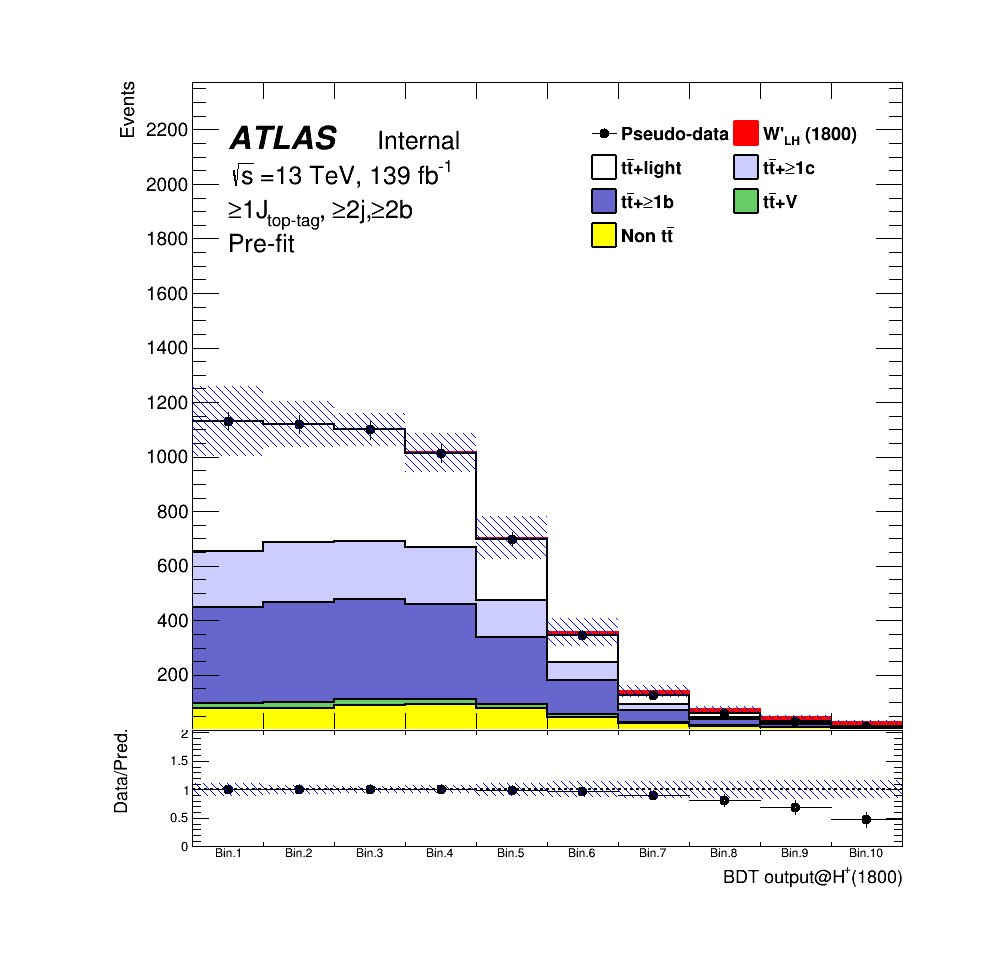
\includegraphics[width=0.45\textwidth]{images/ProfileLHFit/Prefit_Wp1800-LH_asimov_SR.png}
  }
  \subfloat[]{
    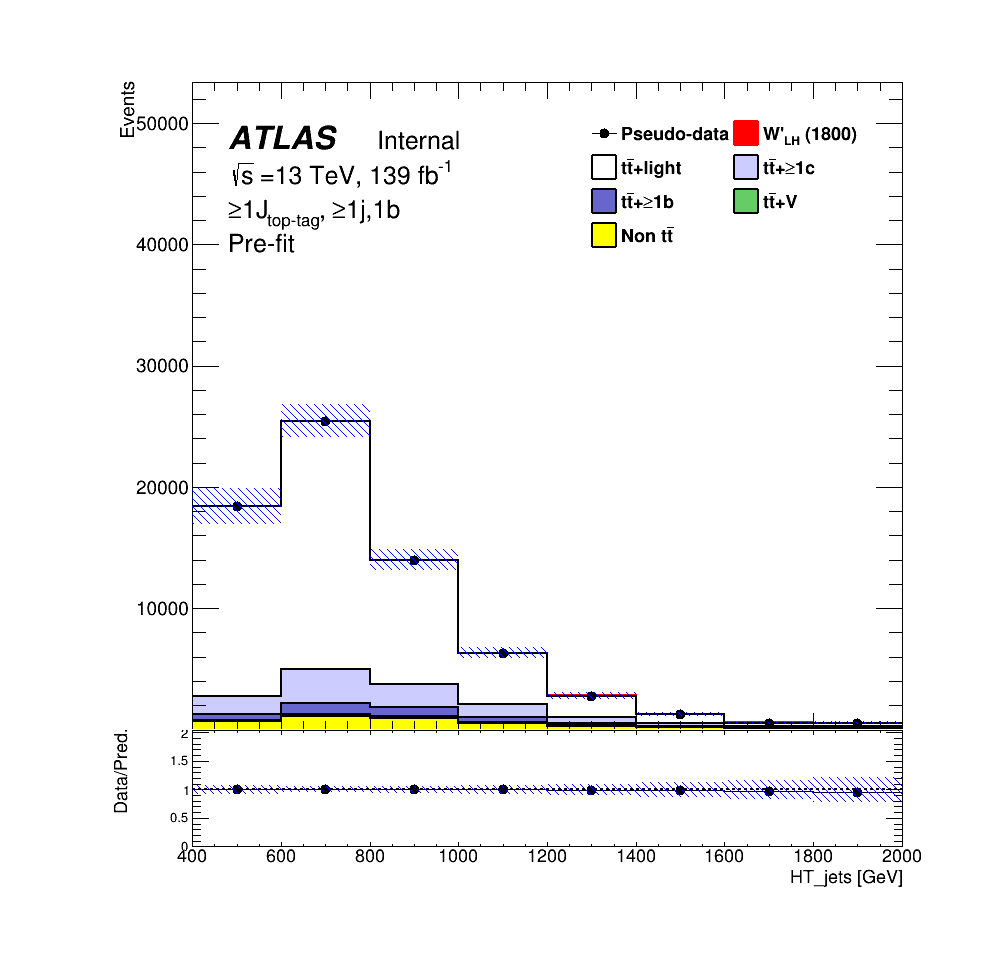
\includegraphics[width=0.45\textwidth]{images/ProfileLHFit/Prefit_Wp1800-LH_asimov_CR.png}
  }
  \caption{Pre-fit plots in the SR (left) and CR (right) for 1800 GeV mass hypothesis of $W'_{\text{L}}$ signal.}
  \label{fig:Prefit_WpLH1800_Asimov}
\end{figure}
\begin{figure}[H]
  \centering
  \subfloat[]{
    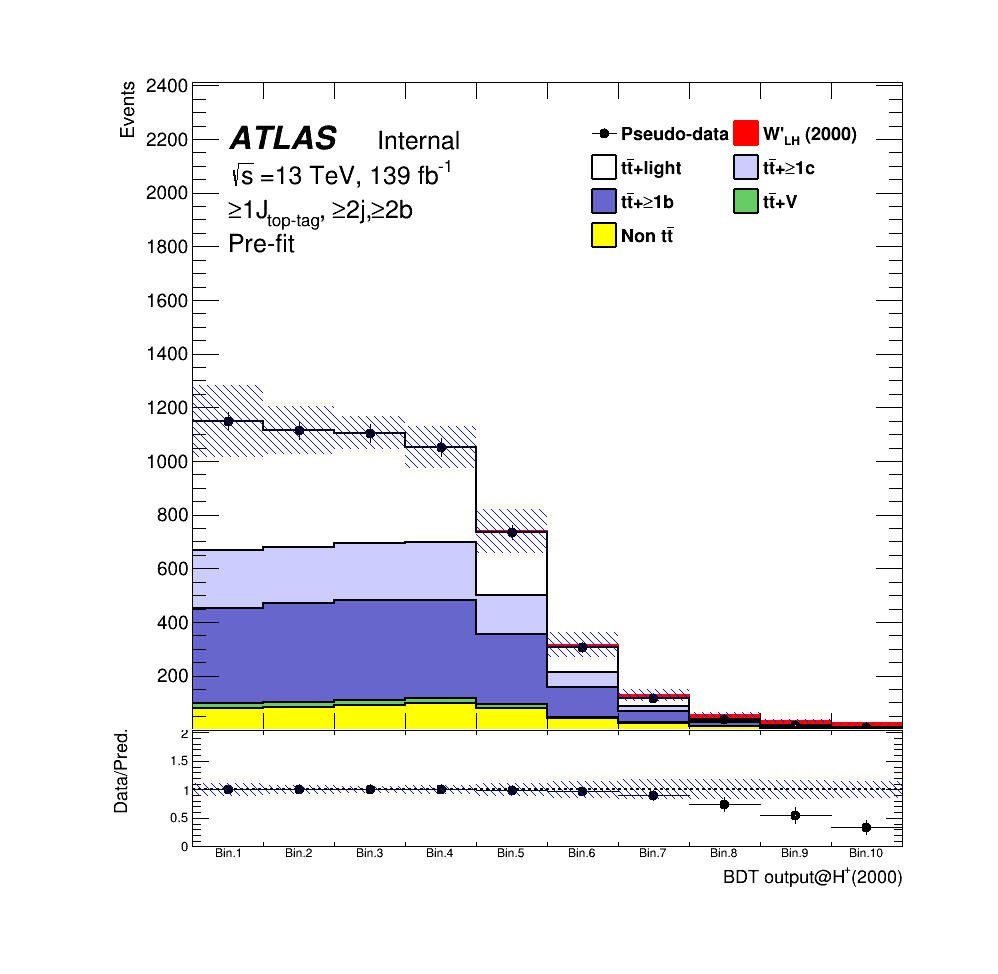
\includegraphics[width=0.45\textwidth]{images/ProfileLHFit/Prefit_Wp2000-LH_asimov_SR.png}
  }
  \subfloat[]{
    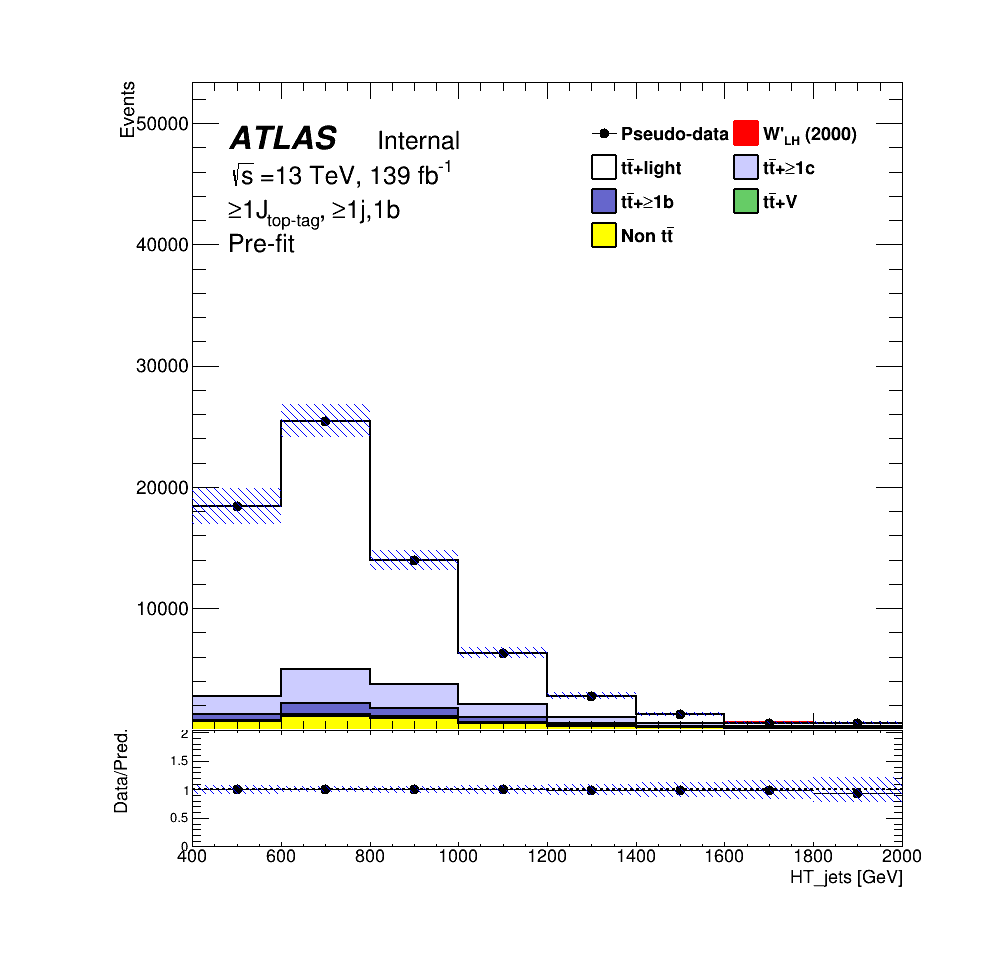
\includegraphics[width=0.45\textwidth]{images/ProfileLHFit/Prefit_Wp2000-LH_asimov_CR.png}
  }
  \caption{Pre-fit plots in the SR (left) and CR (right) for 2000 GeV mass hypothesis of $W'_{\text{L}}$ signal.}
  \label{fig:Prefit_WpLH2000_Asimov}
\end{figure}
\begin{figure}[H]
  \centering
  \subfloat[]{
    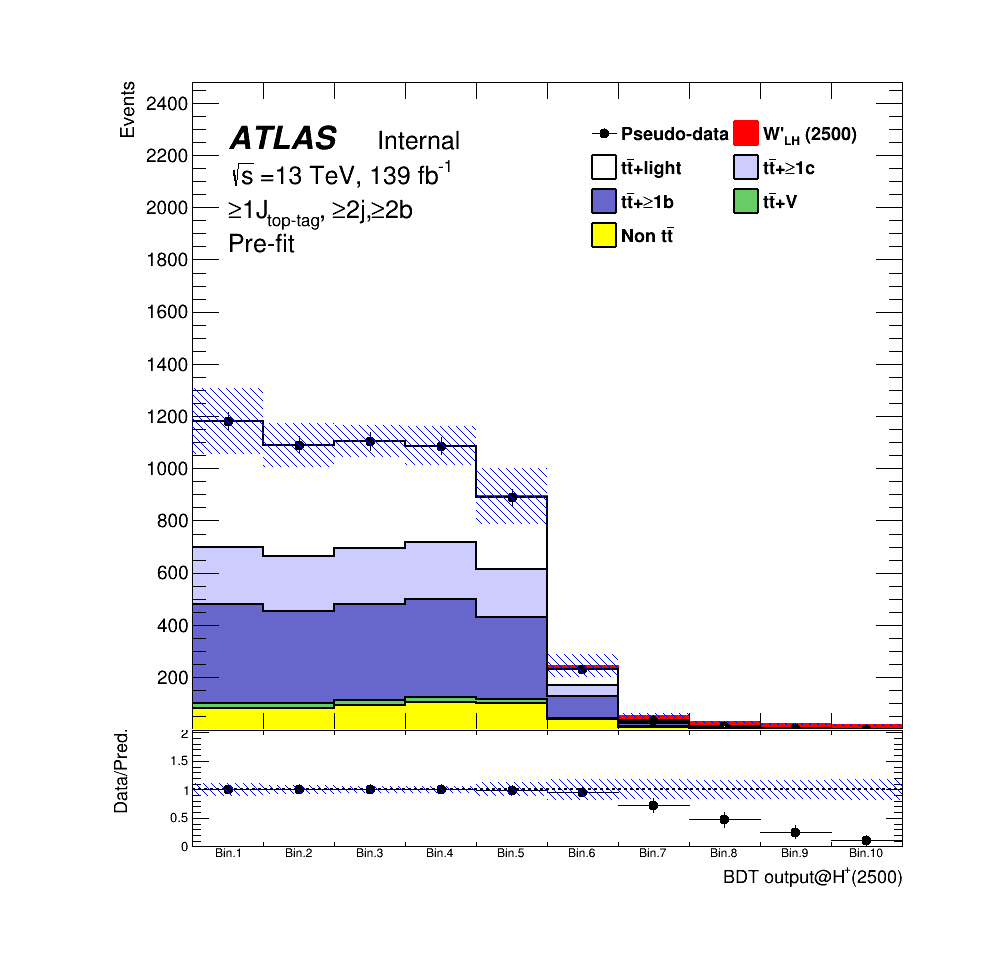
\includegraphics[width=0.45\textwidth]{images/ProfileLHFit/Prefit_Wp2500-LH_asimov_SR.png}
  }
  \subfloat[]{
    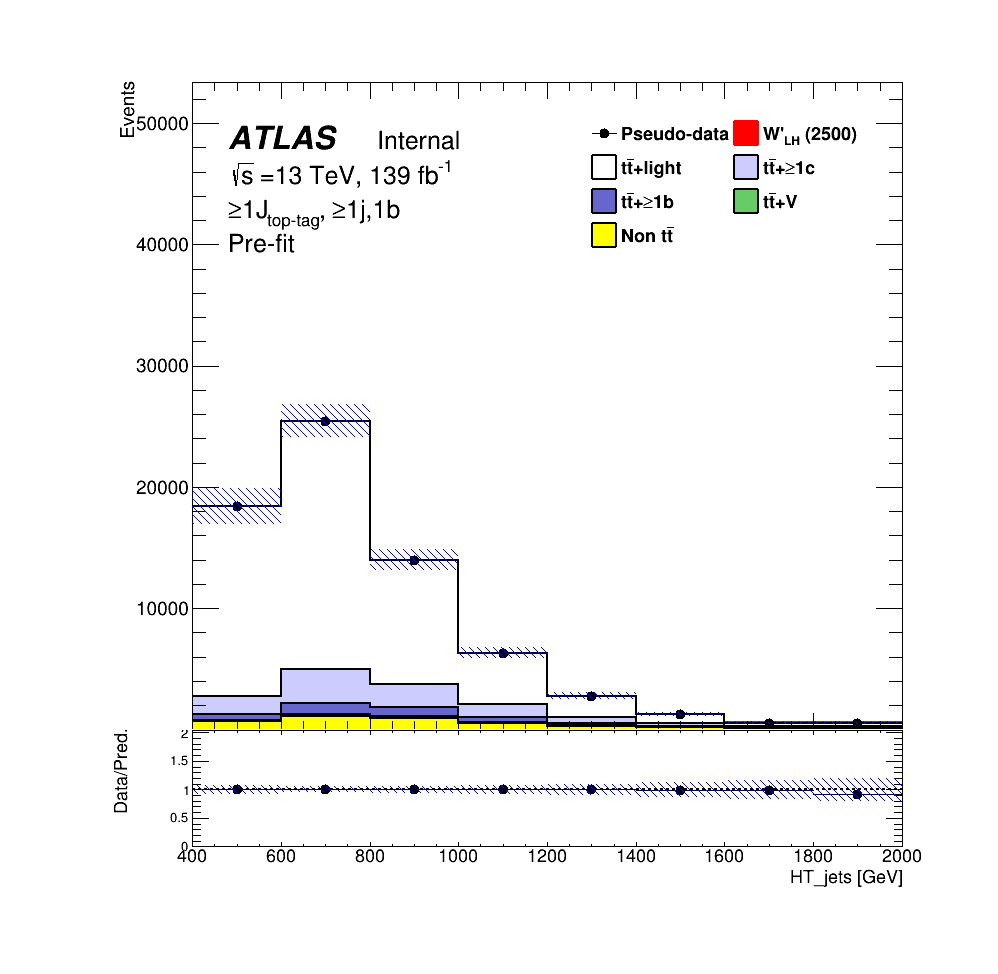
\includegraphics[width=0.45\textwidth]{images/ProfileLHFit/Prefit_Wp2500-LH_asimov_CR.png}
  }
  \caption{Pre-fit plots in the SR (left) and CR (right) for 2500 GeV mass hypothesis of $W'_{\text{L}}$ signal.}
  \label{fig:Prefit_WpLH2500_Asimov}
\end{figure}
\begin{figure}[H]
  \centering
  \subfloat[]{
    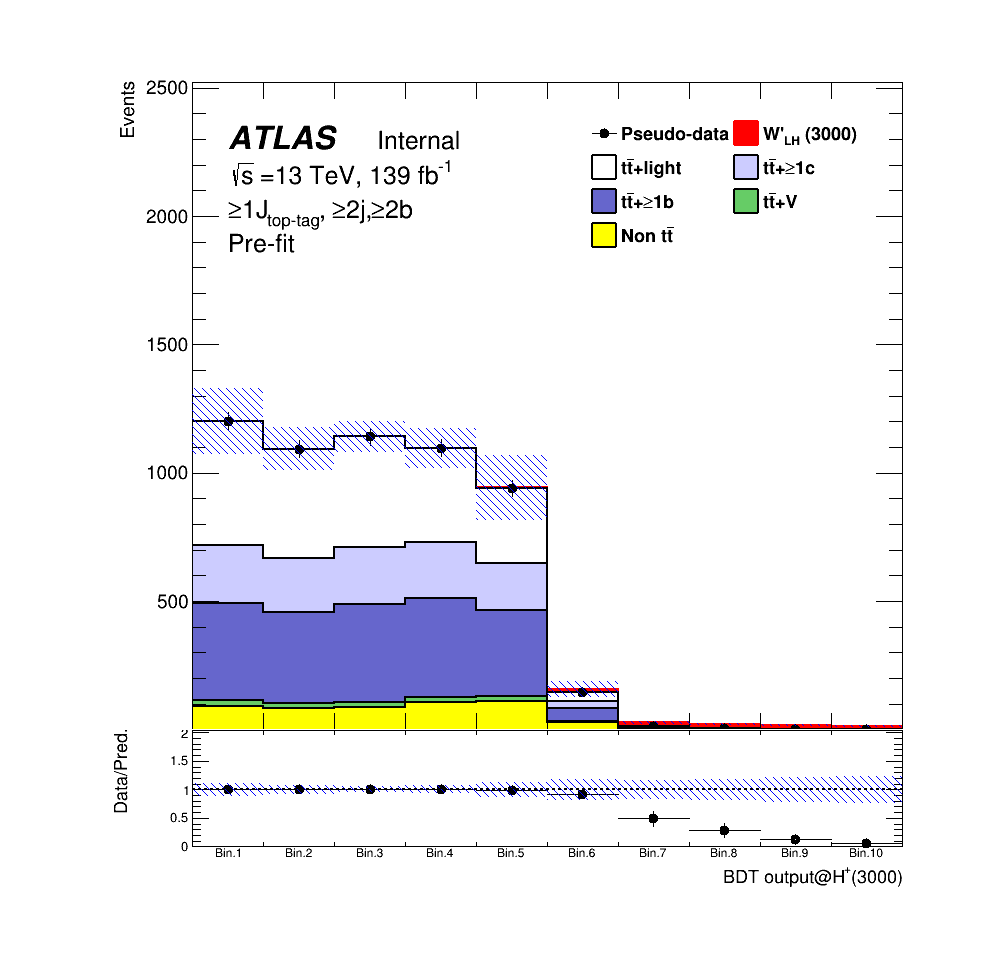
\includegraphics[width=0.45\textwidth]{images/ProfileLHFit/Prefit_Wp3000-LH_asimov_SR.png}
  }
  \subfloat[]{
    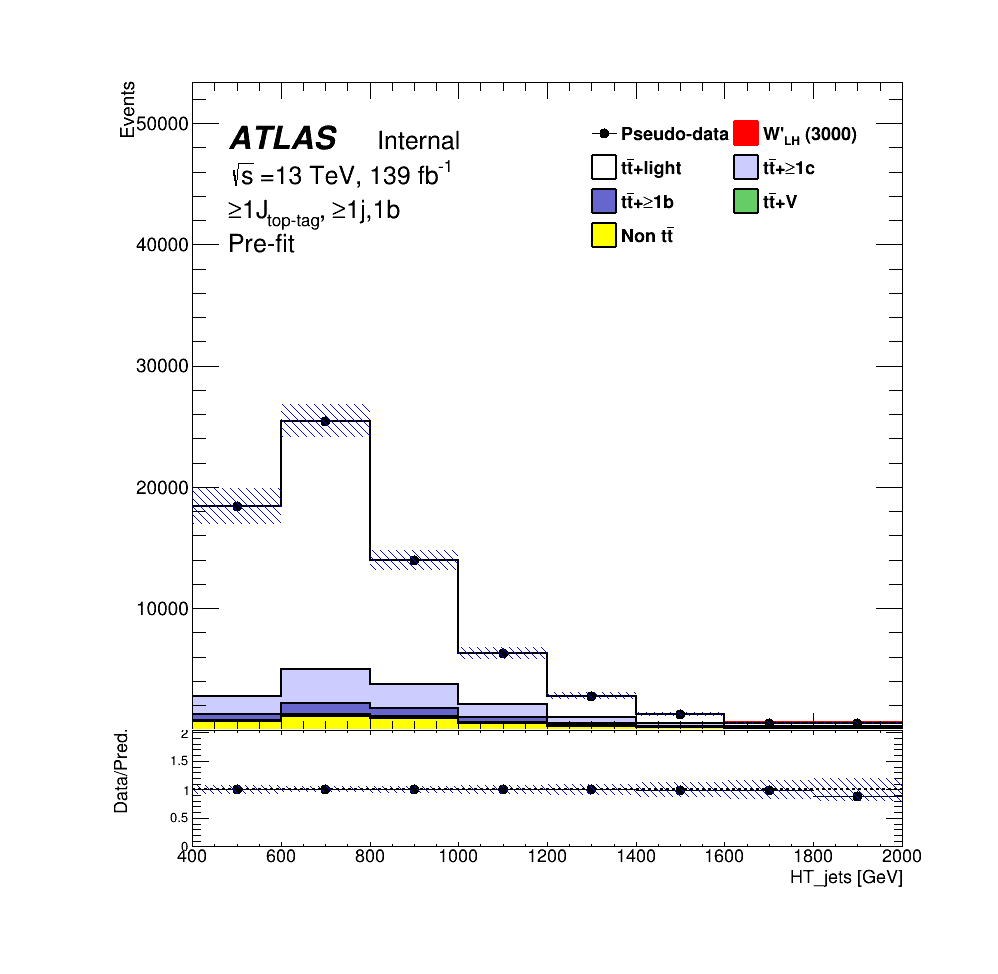
\includegraphics[width=0.45\textwidth]{images/ProfileLHFit/Prefit_Wp3000-LH_asimov_CR.png}
  }
  \caption{Pre-fit plots in the SR (left) and CR (right) for 3000 GeV mass hypothesis of $W'_{\text{L}}$ signal.}
  \label{fig:Prefit_WpLH3000_Asimov}
\end{figure}
\begin{figure}[H]
  \centering
  \subfloat[]{
    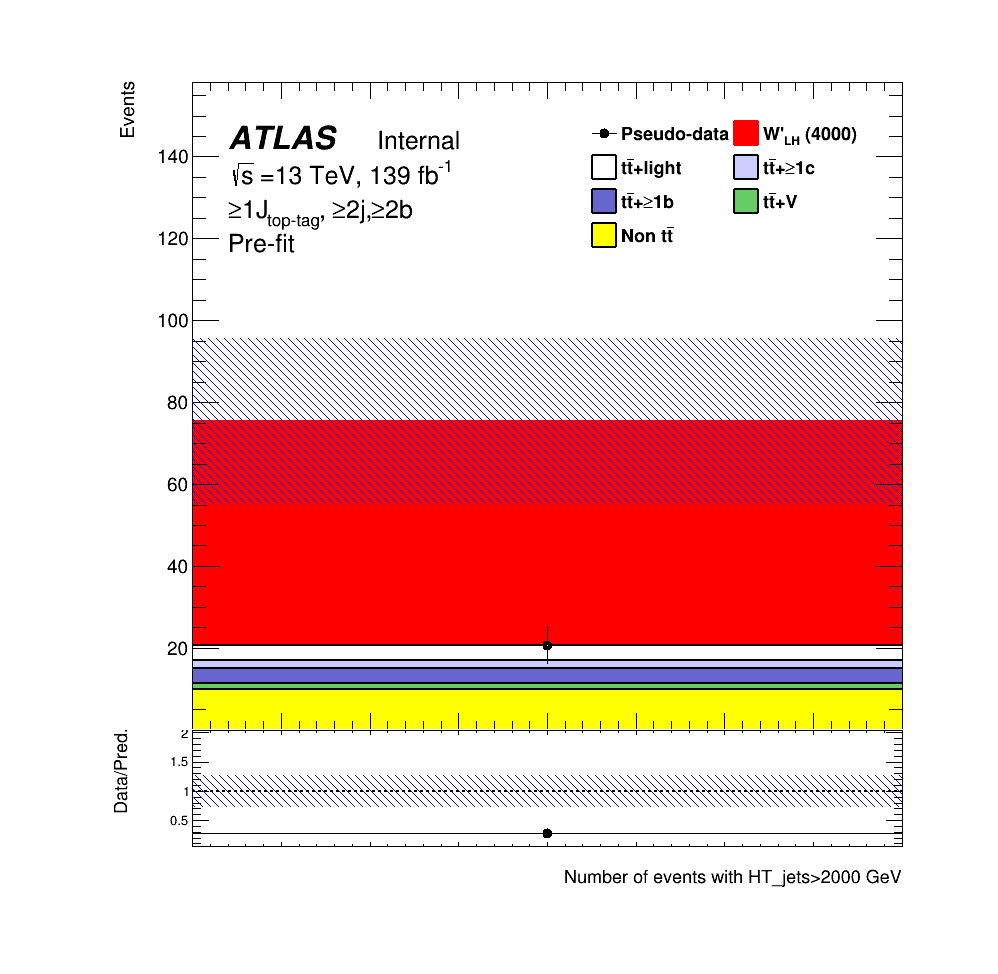
\includegraphics[width=0.45\textwidth]{images/ProfileLHFit/Prefit_Wp4000-LH_asimov_SR.png}
  }\par
  \subfloat[]{
    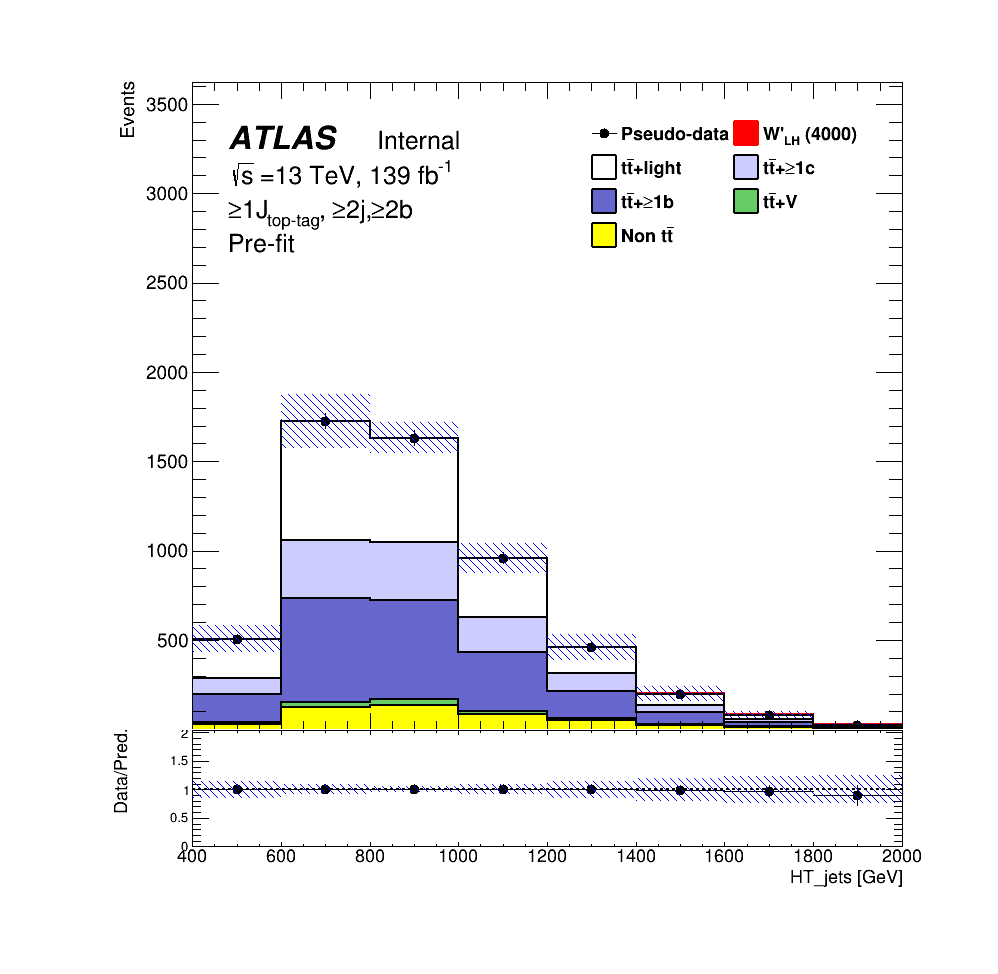
\includegraphics[width=0.45\textwidth]{images/ProfileLHFit/Prefit_Wp4000-LH_asimov_CR1.png}
  }
  \subfloat[]{
    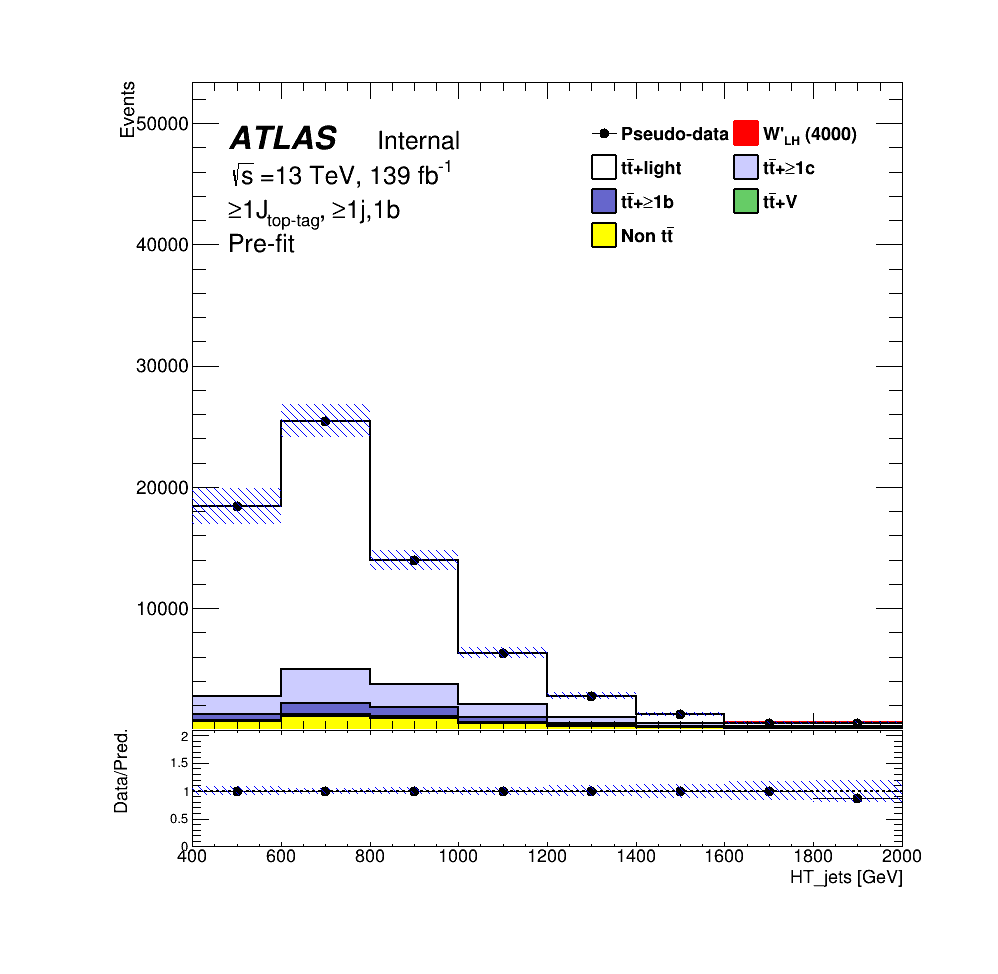
\includegraphics[width=0.45\textwidth]{images/ProfileLHFit/Prefit_Wp4000-LH_asimov_CR2.png}
  }
  \caption{Pre-fit plots in the SR (top), CR1 (bottom-left), and CR2 (bottom-right) for 4000 GeV mass hypothesis of $W'_{\text{L}}$ signal.}
  \label{fig:Prefit_WpLH4000_Asimov}
\end{figure}

% --- Pre-fit plots for W'-RH
\begin{figure}[H]
  \centering
  \subfloat[]{
    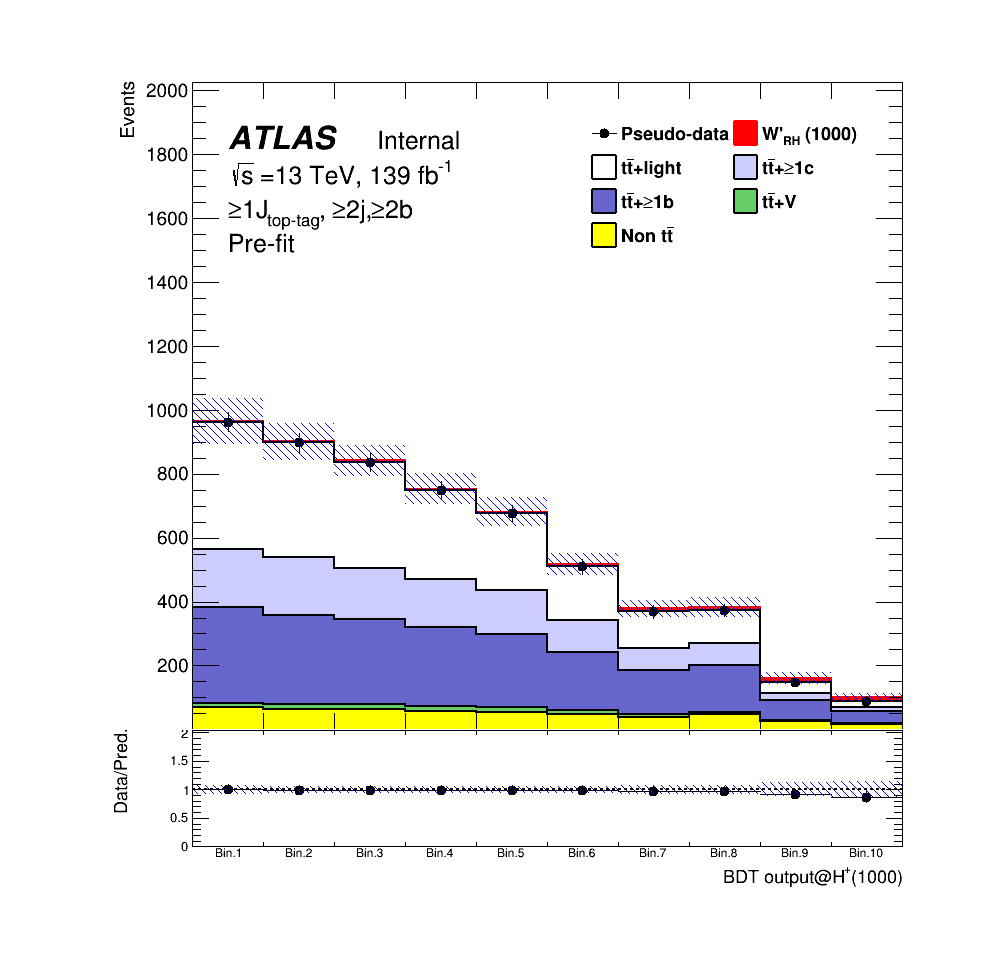
\includegraphics[width=0.45\textwidth]{images/ProfileLHFit/Prefit_Wp1000-RH_asimov_SR.png}
  }
  \subfloat[]{
    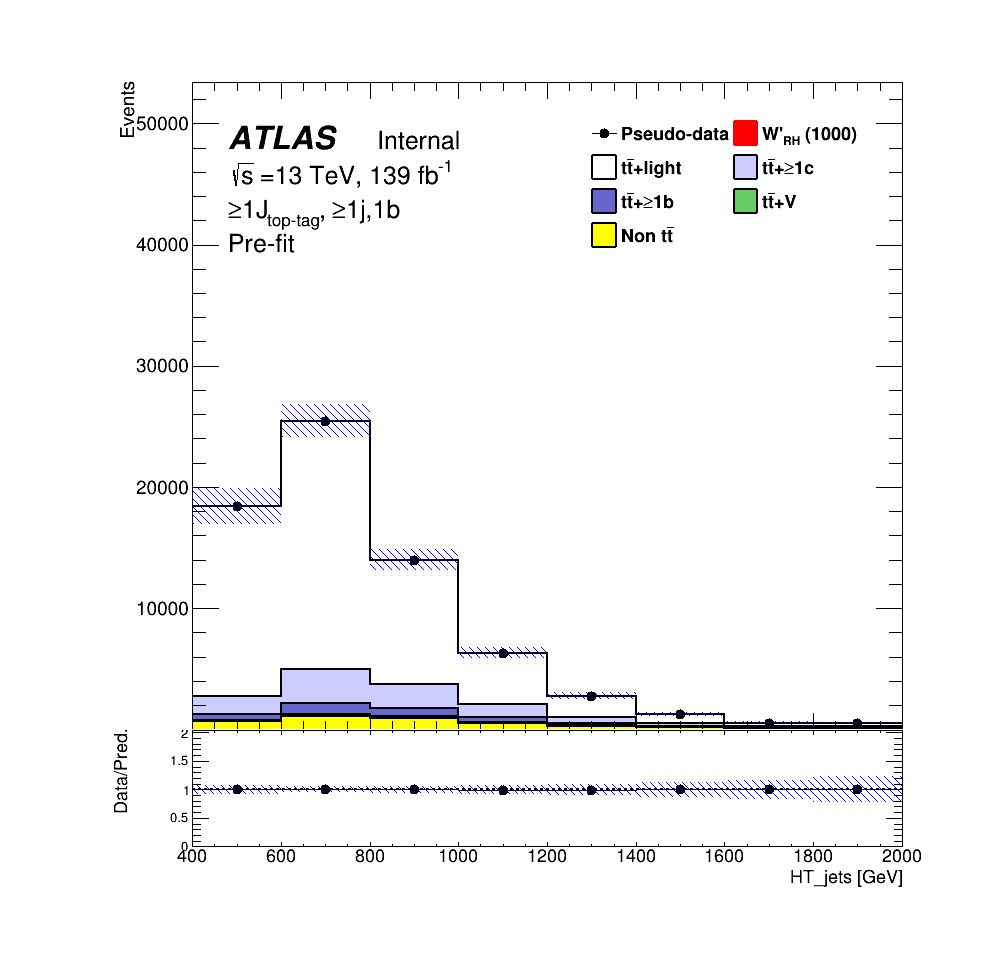
\includegraphics[width=0.45\textwidth]{images/ProfileLHFit/Prefit_Wp1000-RH_asimov_CR.png}
  }
  \caption{Pre-fit plots in the SR (left) and CR (right) for 1000 GeV mass hypothesis of $W'_{\text{R}}$ signal.}
  \label{fig:Prefit_WpRH1000_Asimov}
\end{figure}
\begin{figure}[H]
  \centering
  \subfloat[]{
    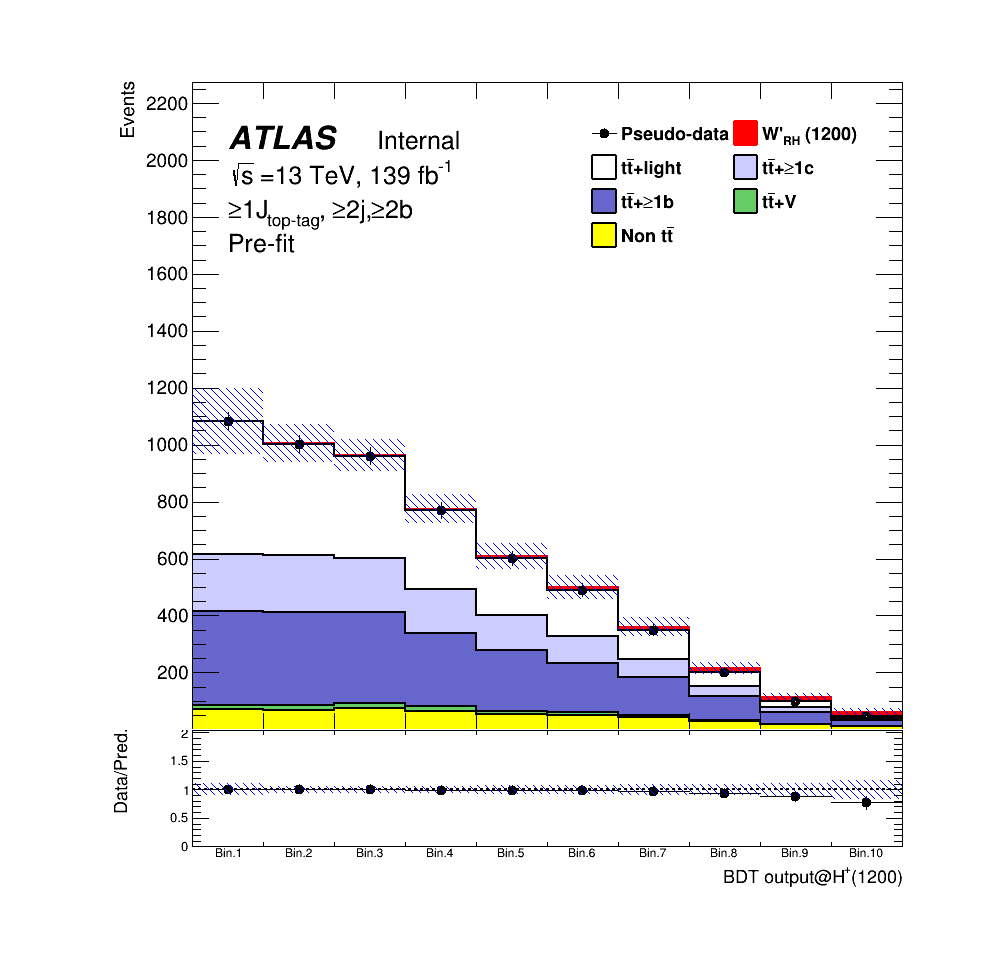
\includegraphics[width=0.45\textwidth]{images/ProfileLHFit/Prefit_Wp1200-RH_asimov_SR.png}
  }
  \subfloat[]{
    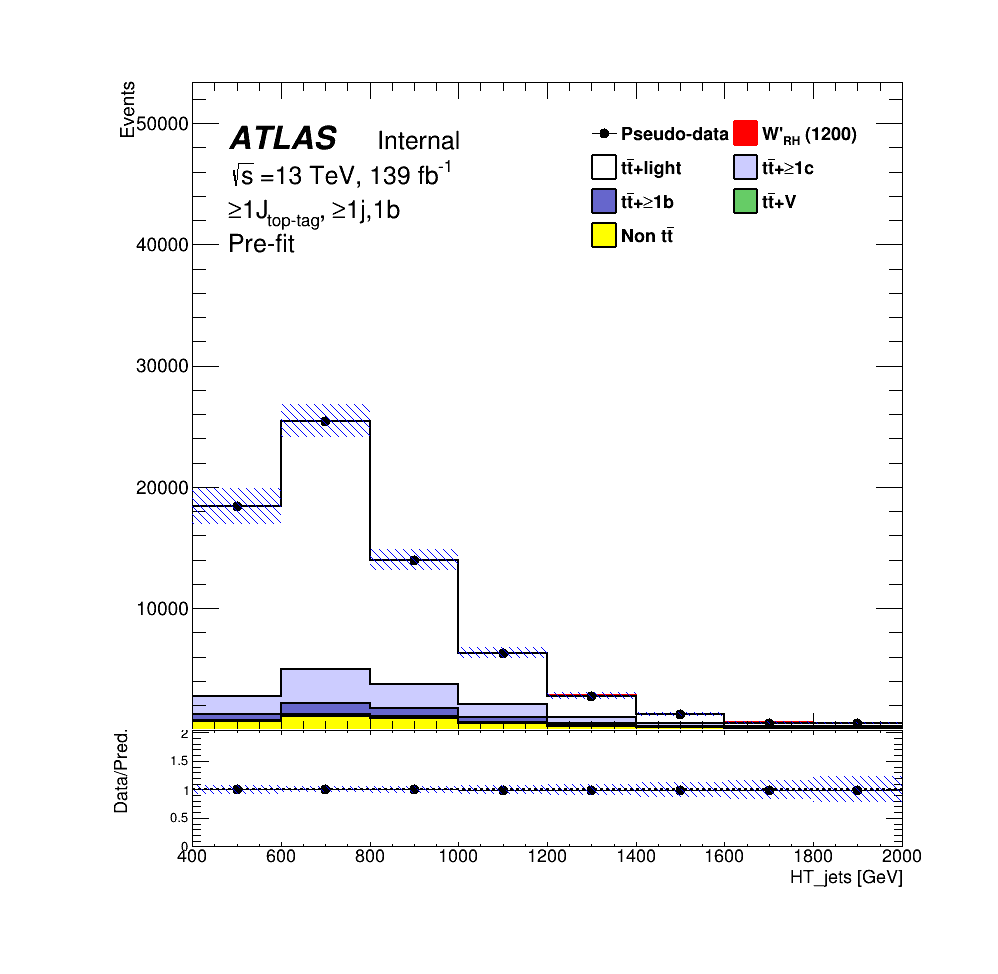
\includegraphics[width=0.45\textwidth]{images/ProfileLHFit/Prefit_Wp1200-RH_asimov_CR.png}
  }
  \caption{Pre-fit plots in the SR (left) and CR (right) for 1200 GeV mass hypothesis of $W'_{\text{R}}$ signal.}
  \label{fig:Prefit_WpRH1200_Asimov}
\end{figure}
\begin{figure}[H]
  \centering
  \subfloat[]{
    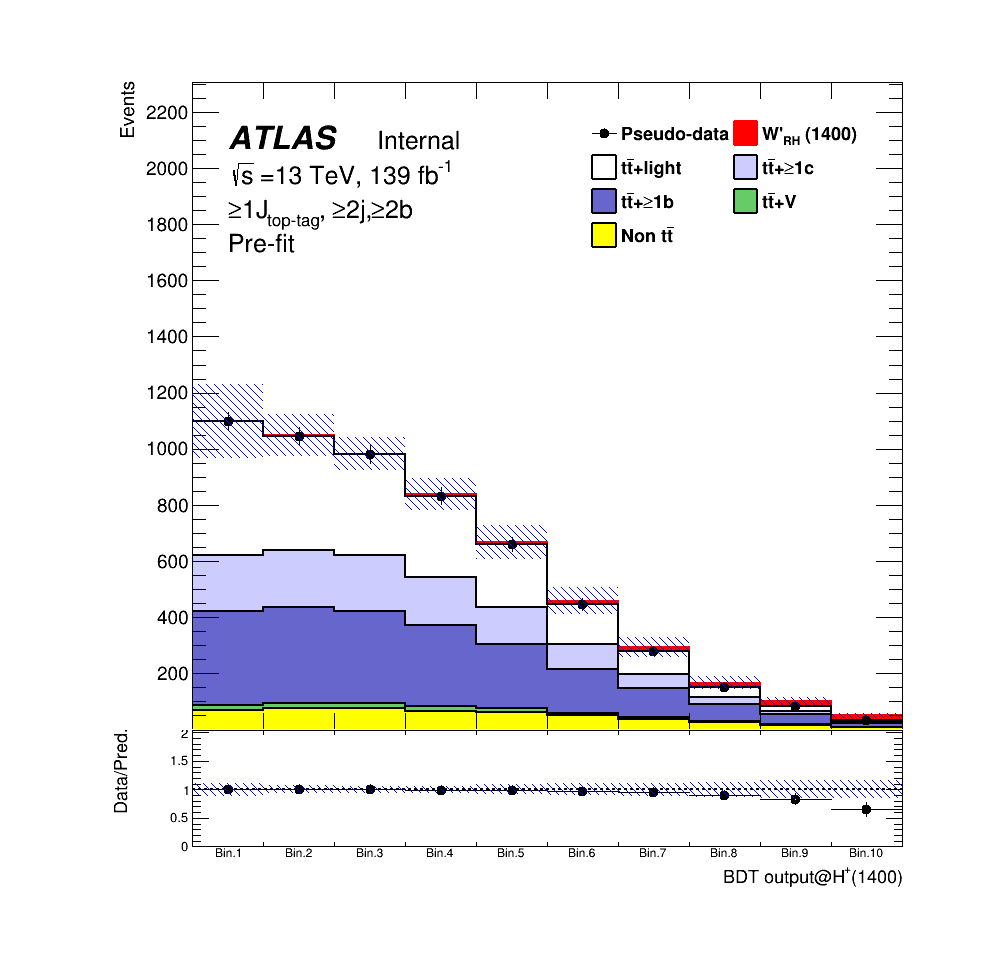
\includegraphics[width=0.45\textwidth]{images/ProfileLHFit/Prefit_Wp1400-RH_asimov_SR.png}
  }
  \subfloat[]{
    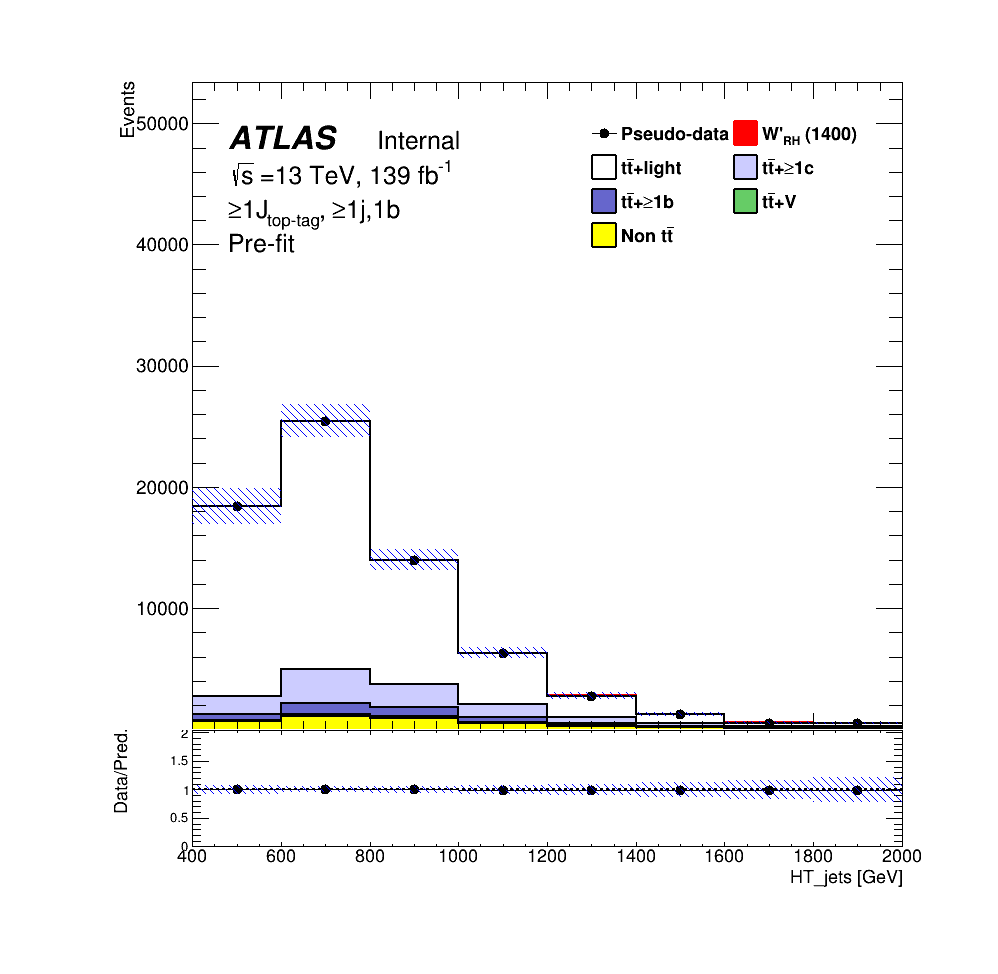
\includegraphics[width=0.45\textwidth]{images/ProfileLHFit/Prefit_Wp1400-RH_asimov_CR.png}
  }
  \caption{Pre-fit plots in the SR (left) and CR (right) for 1400 GeV mass hypothesis of $W'_{\text{R}}$ signal.}
  \label{fig:Prefit_WpRH1400_Asimov}
\end{figure}
\begin{figure}[H]
  \centering
  \subfloat[]{
    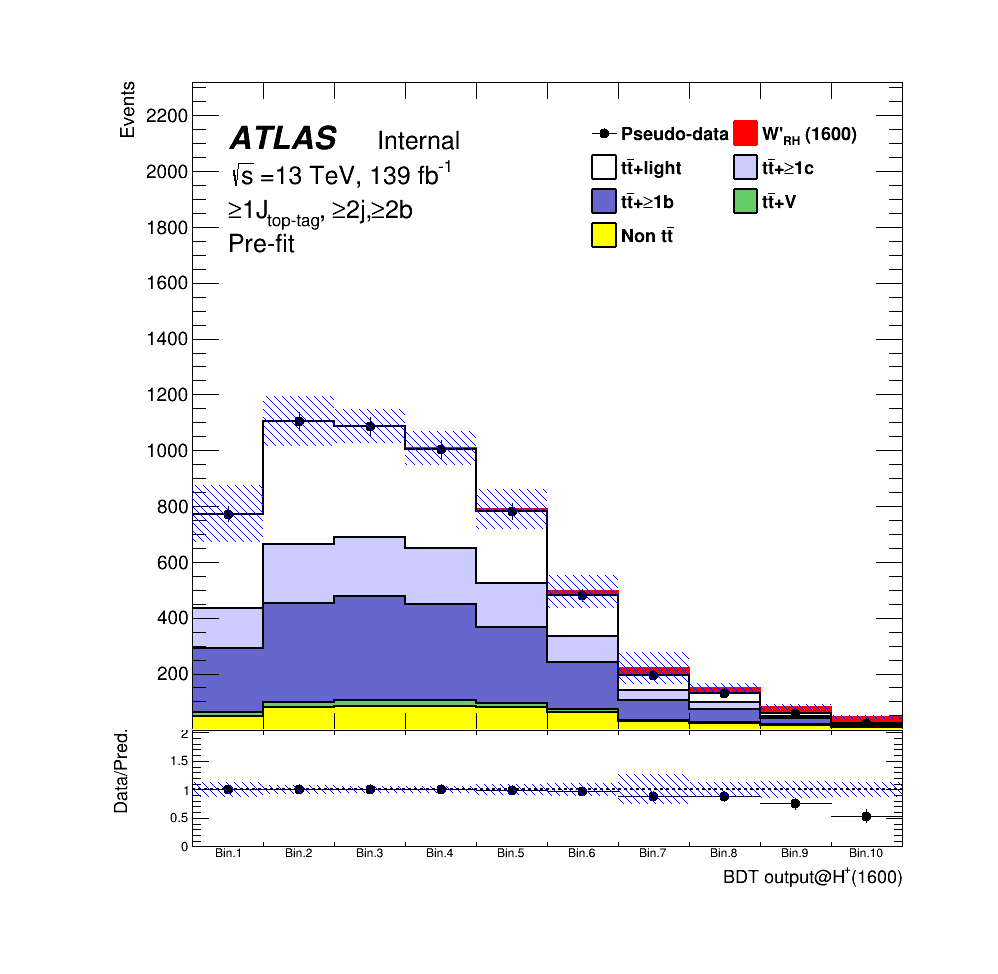
\includegraphics[width=0.45\textwidth]{images/ProfileLHFit/Prefit_Wp1600-RH_asimov_SR.png}
  }
  \subfloat[]{
    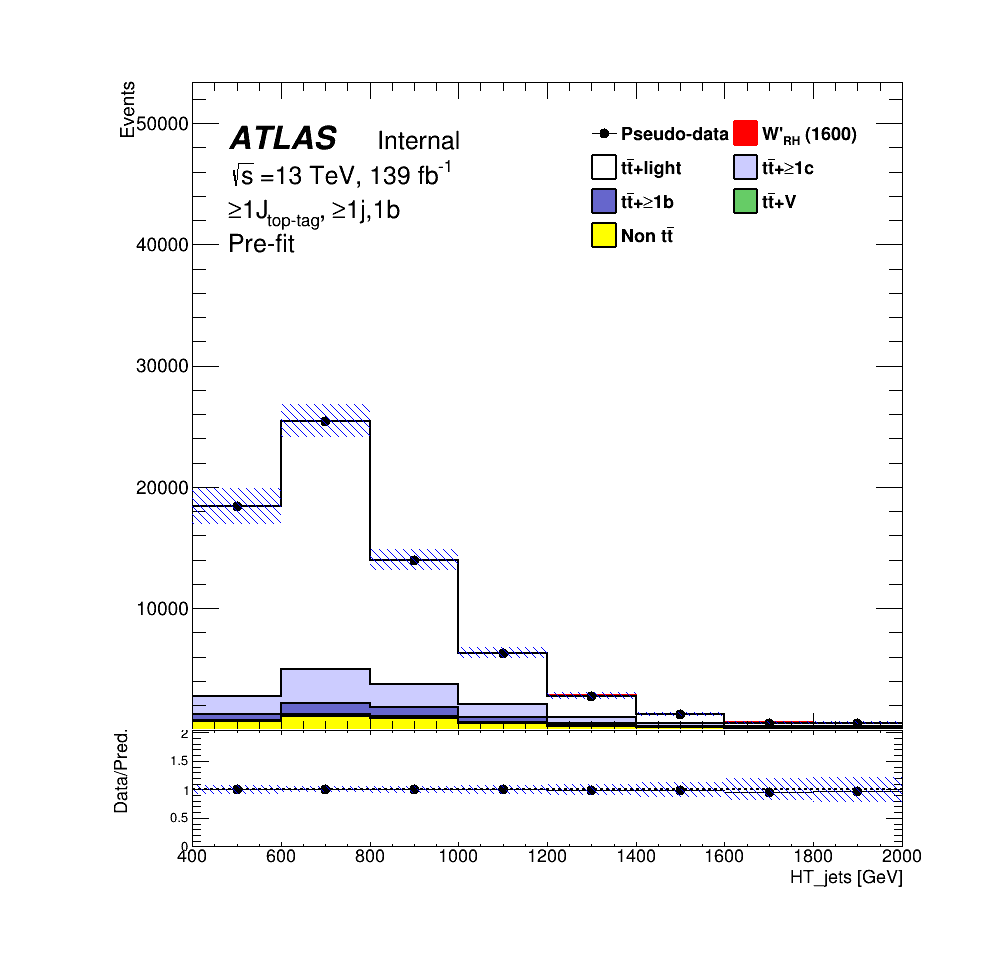
\includegraphics[width=0.45\textwidth]{images/ProfileLHFit/Prefit_Wp1600-RH_asimov_CR.png}
  }
  \caption{Pre-fit plots in the SR (left) and CR (right) for 1600 GeV mass hypothesis of $W'_{\text{R}}$ signal.}
  \label{fig:Prefit_WpRH1600_Asimov}
\end{figure}
\begin{figure}[H]
  \centering
  \subfloat[]{
    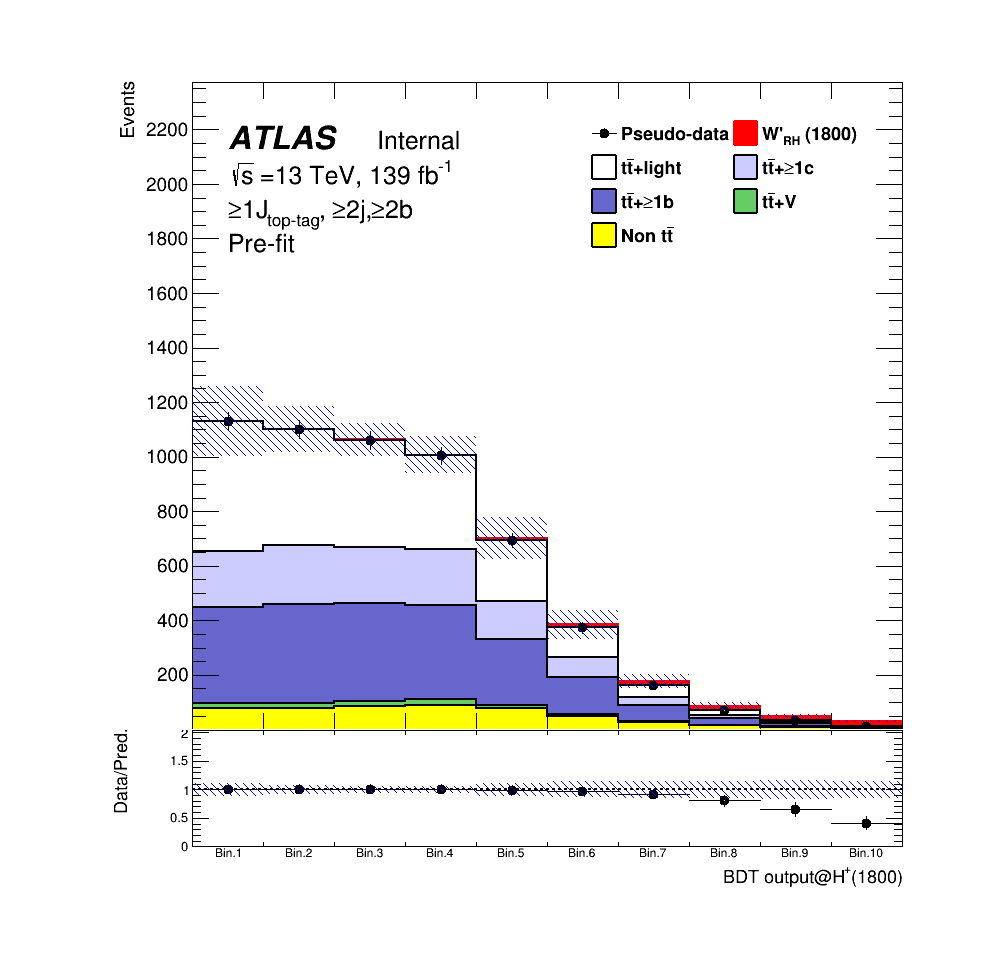
\includegraphics[width=0.45\textwidth]{images/ProfileLHFit/Prefit_Wp1800-RH_asimov_SR.png}
  }
  \subfloat[]{
    \includegraphics[width=0.45\textwidth]{images/ProfileLHFit/Prefit_Wp1800-RH_asimov_CR.png}
  }
  \caption{Pre-fit plots in the SR (left) and CR (right) for 1800 GeV mass hypothesis of $W'_{\text{R}}$ signal.}
  \label{fig:Prefit_WpRH1800_Asimov}
\end{figure}
\begin{figure}[H]
  \centering
  \subfloat[]{
    \includegraphics[width=0.45\textwidth]{images/ProfileLHFit/Prefit_Wp2000-RH_asimov_SR.png}
  }
  \subfloat[]{
    \includegraphics[width=0.45\textwidth]{images/ProfileLHFit/Prefit_Wp2000-RH_asimov_CR.png}
  }
  \caption{Pre-fit plots in the SR (left) and CR (right) for 2000 GeV mass hypothesis of $W'_{\text{R}}$ signal.}
  \label{fig:Prefit_WpRH2000_Asimov}
\end{figure}
\begin{figure}[H]
  \centering
  \subfloat[]{
    \includegraphics[width=0.45\textwidth]{images/ProfileLHFit/Prefit_Wp2500-RH_asimov_SR.png}
  }
  \subfloat[]{
    \includegraphics[width=0.45\textwidth]{images/ProfileLHFit/Prefit_Wp2500-RH_asimov_CR.png}
  }
  \caption{Pre-fit plots in the SR (left) and CR (right) for 2500 GeV mass hypothesis of $W'_{\text{R}}$ signal.}
  \label{fig:Prefit_WpRH2500_Asimov}
\end{figure}
\begin{figure}[H]
  \centering
  \subfloat[]{
    \includegraphics[width=0.45\textwidth]{images/ProfileLHFit/Prefit_Wp3000-RH_asimov_SR.png}
  }
  \subfloat[]{
    \includegraphics[width=0.45\textwidth]{images/ProfileLHFit/Prefit_Wp3000-RH_asimov_CR.png}
  }
  \caption{Pre-fit plots in the SR (left) and CR (right) for 3000 GeV mass hypothesis of $W'_{\text{R}}$ signal.}
  \label{fig:Prefit_WpRH3000_Asimov}
\end{figure}
\begin{figure}[H]
  \centering
  \subfloat[]{
    \includegraphics[width=0.45\textwidth]{images/ProfileLHFit/Prefit_Wp4000-RH_asimov_SR.png}
  }\par
  \subfloat[]{
    \includegraphics[width=0.45\textwidth]{images/ProfileLHFit/Prefit_Wp4000-RH_asimov_CR1.png}
  }
  \subfloat[]{
    \includegraphics[width=0.45\textwidth]{images/ProfileLHFit/Prefit_Wp4000-RH_asimov_CR2.png}
  }
  \caption{Pre-fit plots in the SR (top), CR1 (bottom-left), and CR2 (bottom-right) for 4000 GeV mass hypothesis of $W'_{\text{R}}$ signal.}
  \label{fig:Prefit_WpRH4000_Asimov}
\end{figure}

\subsubsection{Asimov fit results}
\label{subsubsec:AsimovFit}
In the following, the results of the fitting to Asimov datasets are presented. Figures \ref{fig:NuisParAndRanking_Hp1000} to \ref{fig:NormFactorsAndCorrMatrix_Hp5000} show the nuisance parameters, normalization factors, correlation matrices, the effect of the different nuisance parameters before and after the fit and post-fit plots from the fits under each $H^{+}$ mass hypotheses. Similarly, Figure \ref{fig:NuisParAndRanking_WpLH1000} to \ref{fig:NormFactorsAndCorrMatrix_WpLH4000} and Figure \ref{fig:NuisParAndRanking_WpRH1000} to \ref{fig:NormFactorsAndCorrMatrix_WpRH4000} show the results from the fits under each $W'_{\text{L}}$ and $W'_{\text{R}}$ mass hypotheses, respectively.

%--- H+
\begin{figure}[H]
  \centering
  \subfloat[Nuisance  parameters]{
    \includegraphics[width=0.45\textwidth]{images/ProfileLHFit/NuisPar_Hp1000.png}
    \label{fig:NuiPar_Hp1000}
  }
  \subfloat[Systematics ranking]{
    \includegraphics[width=0.45\textwidth]{images/ProfileLHFit/Ranking_Hp1000.png}
    \label{fig:Ranking_Hp1000}
  }
  \caption{Nuisance parameters (left) and ranking plot (right) of the effect of various nuisance parameters before and after the fit for the 1000 GeV $H^{+}$ mass hypotheses.}
  \label{fig:NuisParAndRanking_Hp1000}
\end{figure}
\begin{figure}[H]
  \centering
  \subfloat[Norm. factors]{
    \includegraphics[width=0.8\textwidth]{images/ProfileLHFit/NormFactors_Hp1000.png}
    \label{fig:NormFactors_Hp1000}
  }\\
  \subfloat[Correlation matrix]{
    \includegraphics[width=0.8\textwidth]{images/ProfileLHFit/CorrMatrix_Hp1000.png}
    \label{fig:CorrMatrix_Hp1000}
  }
  \caption{Signal strength and normalization factors (top) and correlation matrix (bottom) for the 1000 GeV $H^{+}$ mass hypotheses.}
  \label{fig:NormFactorsAndCorrMatrix_Hp1000}
\end{figure}
\begin{figure}[H]
  \centering
  \subfloat[Nuisance  parameters]{
    \includegraphics[width=0.4\textwidth]{images/ProfileLHFit/NuisPar_Hp1200.png}
  }
  \subfloat[Systematics ranking]{
    \includegraphics[width=0.45\textwidth]{images/ProfileLHFit/Ranking_Hp1200.png}
  }
  \caption{Nuisance parameters (left) and ranking plot (right) of the effect of various nuisance parameters before and after the fit for the 1200 GeV $H^{+}$ mass hypotheses.}
\end{figure}
\begin{figure}[H]
  \centering
  \subfloat[Norm. factors]{
    \includegraphics[width=0.8\textwidth]{images/ProfileLHFit/NormFactors_Hp1200.png}
  }\\
  \subfloat[Correlation matrix]{
    \includegraphics[width=0.8\textwidth]{images/ProfileLHFit/CorrMatrix_Hp1200.png}
  }
  \caption{Signal strength and normalization factors (top) and correlation matrix (bottom) for the 1200 GeV $H^{+}$ mass hypotheses.}
\end{figure}
\begin{figure}[H]
  \centering
  \subfloat[Nuisance  parameters]{
    \includegraphics[width=0.45\textwidth]{images/ProfileLHFit/NuisPar_Hp1400.png}
  }
  \subfloat[Systematics ranking]{
    \includegraphics[width=0.45\textwidth]{images/ProfileLHFit/Ranking_Hp1400.png}
  }
  \caption{Nuisance parameters (left) and ranking plot (right) of the effect of various nuisance parameters before and after the fit for the 1400 GeV $H^{+}$ mass hypotheses.}
\end{figure}
\begin{figure}[H]
  \centering
  \subfloat[Norm. factors]{
    \includegraphics[width=0.8\textwidth]{images/ProfileLHFit/NormFactors_Hp1400.png}
  }\\
  \subfloat[Correlation matrix]{
    \includegraphics[width=0.8\textwidth]{images/ProfileLHFit/CorrMatrix_Hp1400.png}
  }
  \caption{Signal strength and normalization factors (top) and correlation matrix (bottom) for the 1400 GeV $H^{+}$ mass hypotheses.}
\end{figure}
\begin{figure}[H]
  \centering
  \subfloat[Nuisance  parameters]{
    \includegraphics[width=0.4\textwidth]{images/ProfileLHFit/NuisPar_Hp1600.png}
  }
  \subfloat[Systematics ranking]{
    \includegraphics[width=0.45\textwidth]{images/ProfileLHFit/Ranking_Hp1600.png}
  }
  \caption{Nuisance parameters (left) and ranking plot (right) of the effect of various nuisance parameters before and after the fit for the 1600 GeV $H^{+}$ mass hypotheses.}
\end{figure}
\begin{figure}[H]
  \centering
  \subfloat[Norm. factors]{
    \includegraphics[width=0.8\textwidth]{images/ProfileLHFit/NormFactors_Hp1600.png}
  }\\
  \subfloat[Correlation matrix]{
    \includegraphics[width=0.8\textwidth]{images/ProfileLHFit/CorrMatrix_Hp1600.png}
  }
  \caption{Signal strength and normalization factors (top) and correlation matrix (bottom) for the 1600 GeV $H^{+}$ mass hypotheses.}
\end{figure}
\begin{figure}[H]
  \centering
  \subfloat[Nuisance  parameters]{
    \includegraphics[width=0.45\textwidth]{images/ProfileLHFit/NuisPar_Hp1800.png}
  }
  \subfloat[Systematics ranking]{
    \includegraphics[width=0.45\textwidth]{images/ProfileLHFit/Ranking_Hp1800.png}
  }
  \caption{Nuisance parameters (left) and ranking plot (right) of the effect of various nuisance parameters before and after the fit for the 1800 GeV $H^{+}$ mass hypotheses.}
\end{figure}
\begin{figure}[H]
  \centering
  \subfloat[Norm. factors]{
    \includegraphics[width=0.8\textwidth]{images/ProfileLHFit/NormFactors_Hp1800.png}
  }\\
  \subfloat[Correlation matrix]{
    \includegraphics[width=0.8\textwidth]{images/ProfileLHFit/CorrMatrix_Hp1800.png}
  }
  \caption{Signal strength and normalization factors (top) and correlation matrix (bottom) for the 1800 GeV $H^{+}$ mass hypotheses.}
\end{figure}
\begin{figure}[H]
  \centering
  \subfloat[Nuisance  parameters]{
    \includegraphics[width=0.45\textwidth]{images/ProfileLHFit/NuisPar_Hp2000.png}
  }
  \subfloat[Systematics ranking]{
    \includegraphics[width=0.45\textwidth]{images/ProfileLHFit/Ranking_Hp2000.png}
  }
  \caption{Nuisance parameters (left) and ranking plot (right) of the effect of various nuisance parameters before and after the fit for the 2000 GeV $H^{+}$ mass hypotheses.}
\end{figure}
\begin{figure}[H]
  \centering
  \subfloat[Norm. factors]{
    \includegraphics[width=0.8\textwidth]{images/ProfileLHFit/NormFactors_Hp2000.png}
  }\\
  \subfloat[Correlation matrix]{
    \includegraphics[width=0.8\textwidth]{images/ProfileLHFit/CorrMatrix_Hp2000.png}
  }
  \caption{Signal strength and normalization factors (top) and correlation matrix (bottom) for the 2000 GeV $H^{+}$ mass hypotheses.}
\end{figure}
\begin{figure}[H]
  \centering
  \subfloat[Nuisance  parameters]{
    \includegraphics[width=0.45\textwidth]{images/ProfileLHFit/NuisPar_Hp2500.png}
  }
  \subfloat[Systematics ranking]{
    \includegraphics[width=0.45\textwidth]{images/ProfileLHFit/Ranking_Hp2500.png}
  }
  \caption{Nuisance parameters (left) and ranking plot (right) of the effect of various nuisance parameters before and after the fit for the 2500 GeV $H^{+}$ mass hypotheses.}
\end{figure}
\begin{figure}[H]
  \centering
  \subfloat[Norm. factors]{
    \includegraphics[width=0.8\textwidth]{images/ProfileLHFit/NormFactors_Hp2500.png}
  }\\
  \subfloat[Correlation matrix]{
    \includegraphics[width=0.8\textwidth]{images/ProfileLHFit/CorrMatrix_Hp2500.png}
  }
  \caption{Signal strength and normalization factors (top) and correlation matrix (bottom) for the 2500 GeV $H^{+}$ mass hypotheses.}
\end{figure}
\begin{figure}[H]
  \centering
  \subfloat[Nuisance  parameters]{
    \includegraphics[width=0.45\textwidth]{images/ProfileLHFit/NuisPar_Hp3000.png}
  }
  \subfloat[Systematics ranking]{
    \includegraphics[width=0.45\textwidth]{images/ProfileLHFit/Ranking_Hp3000.png}
  }
  \caption{Nuisance parameters (left) and ranking plot (right) of the effect of various nuisance parameters before and after the fit for the 3000 GeV $H^{+}$ mass hypotheses.}
\end{figure}
\begin{figure}[H]
  \centering
  \subfloat[Norm. factors]{
    \includegraphics[width=0.8\textwidth]{images/ProfileLHFit/NormFactors_Hp3000.png}
  }\\
  \subfloat[Correlation matrix]{
    \includegraphics[width=0.8\textwidth]{images/ProfileLHFit/CorrMatrix_Hp3000.png}
  }
  \caption{Signal strength and normalization factors (top) and correlation matrix (bottom) for the 3000 GeV $H^{+}$ mass hypotheses.}
\end{figure}
\begin{figure}[H]
  \centering
  \subfloat[Nuisance  parameters]{
    \includegraphics[width=0.33\textwidth]{images/ProfileLHFit/NuisPar_Hp4000.png}
  }
  \subfloat[Systematics ranking]{
    \includegraphics[width=0.45\textwidth]{images/ProfileLHFit/Ranking_Hp4000.png}
  }
  \caption{Nuisance parameters (left) and ranking plot (right) of the effect of various nuisance parameters before and after the fit for the 4000 GeV $H^{+}$ mass hypotheses.}
\end{figure}
\begin{figure}[H]
  \centering
  \subfloat[Norm. factors]{
    \includegraphics[width=0.8\textwidth]{images/ProfileLHFit/NormFactors_Hp4000.png}
  }\\
  \subfloat[Correlation matrix]{
    \includegraphics[width=0.8\textwidth]{images/ProfileLHFit/CorrMatrix_Hp4000.png}
  }
  \caption{Signal strength and normalization factors (top) and correlation matrix (bottom) for the 4000 GeV $H^{+}$ mass hypotheses.}
\end{figure}
\begin{figure}[H]
  \centering
  \subfloat[Nuisance  parameters]{
    \includegraphics[width=0.33\textwidth]{images/ProfileLHFit/NuisPar_Hp5000.png}
  }
  \subfloat[Systematics ranking]{
    \includegraphics[width=0.45\textwidth]{images/ProfileLHFit/Ranking_Hp5000.png}
  }
  \caption{Nuisance parameters (left) and ranking plot (right) of the effect of various nuisance parameters before and after the fit for the 5000 GeV $H^{+}$ mass hypotheses.}
\end{figure}
\begin{figure}[H]
  \centering
  \subfloat[Norm. factors]{
    \includegraphics[width=0.8\textwidth]{images/ProfileLHFit/NormFactors_Hp5000.png}
  }\\
  \subfloat[Correlation matrix]{
    \includegraphics[width=0.8\textwidth]{images/ProfileLHFit/CorrMatrix_Hp5000.png}
  }
  \caption{Signal strength and normalization factors (top) and correlation matrix (bottom) for the 5000 GeV $H^{+}$ mass hypotheses.}
  \label{fig:NormFactorsAndCorrMatrix_Hp5000}
\end{figure}

%--- W-LH
\begin{figure}[H]
  \centering
  \subfloat[Nuisance  parameters]{
    \includegraphics[width=0.45\textwidth]{images/ProfileLHFit/NuisPar_WpLH1000.png}
  }
  \subfloat[Systematics ranking]{
    \includegraphics[width=0.45\textwidth]{images/ProfileLHFit/Ranking_WpLH1000.png}
  }
  \caption{Nuisance parameters (left) and ranking plot (right) of the effect of various nuisance parameters before and after the fit for the 1000 GeV $W'_{\text{L}}$ mass hypotheses.}
  \label{fig:NuisParAndRanking_WpLH1000}
\end{figure}
\begin{figure}[H]
  \centering
  \subfloat[Norm. factors]{
    \includegraphics[width=0.8\textwidth]{images/ProfileLHFit/NormFactors_WpLH1000.png}
  }\\
  \subfloat[Correlation matrix]{
    \includegraphics[width=0.8\textwidth]{images/ProfileLHFit/CorrMatrix_WpLH1000.png}
  }
  \caption{Signal strength and normalization factors (top) and correlation matrix (bottom) for the 1000 GeV $W'_{\text{L}}$ mass hypotheses.}
  \label{fig:NormFactorsAndCorrMatrix_Hp1000}
\end{figure}
\begin{figure}[H]
  \centering
  \subfloat[Nuisance  parameters]{
    \includegraphics[width=0.45\textwidth]{images/ProfileLHFit/NuisPar_WpLH1200.png}
  }
  \subfloat[Systematics ranking]{
    \includegraphics[width=0.45\textwidth]{images/ProfileLHFit/Ranking_WpLH1200.png}
  }
  \caption{Nuisance parameters (left) and ranking plot (right) of the effect of various nuisance parameters before and after the fit for the 1200 GeV $W'_{\text{L}}$ mass hypotheses.}
  \label{fig:NuisParAndRanking_WpLH1200}
\end{figure}
\begin{figure}[H]
  \centering
  \subfloat[Norm. factors]{
    \includegraphics[width=0.8\textwidth]{images/ProfileLHFit/NormFactors_WpLH1200.png}
  }\\
  \subfloat[Correlation matrix]{
    \includegraphics[width=0.8\textwidth]{images/ProfileLHFit/CorrMatrix_WpLH1200.png}
  }
  \caption{Signal strength and normalization factors (top) and correlation matrix (bottom) for the 1200 GeV $W'_{\text{L}}$ mass hypotheses.}
  \label{fig:NormFactorsAndCorrMatrix_Hp1200}
\end{figure}
\begin{figure}[H]
  \centering
  \subfloat[Nuisance  parameters]{
    \includegraphics[width=0.45\textwidth]{images/ProfileLHFit/NuisPar_WpLH1400.png}
  }
  \subfloat[Systematics ranking]{
    \includegraphics[width=0.45\textwidth]{images/ProfileLHFit/Ranking_WpLH1400.png}
  }
  \caption{Nuisance parameters (left) and ranking plot (right) of the effect of various nuisance parameters before and after the fit for the 1400 GeV $W'_{\text{L}}$ mass hypotheses.}
  \label{fig:NuisParAndRanking_WpLH1400}
\end{figure}
\begin{figure}[H]
  \centering
  \subfloat[Norm. factors]{
    \includegraphics[width=0.8\textwidth]{images/ProfileLHFit/NormFactors_WpLH1400.png}
  }\\
  \subfloat[Correlation matrix]{
    \includegraphics[width=0.8\textwidth]{images/ProfileLHFit/CorrMatrix_WpLH1400.png}
  }
  \caption{Signal strength and normalization factors (top) and correlation matrix (bottom) for the 1400 GeV $W'_{\text{L}}$ mass hypotheses.}
  \label{fig:NormFactorsAndCorrMatrix_Hp1400}
\end{figure}
\begin{figure}[H]
  \centering
  \subfloat[Nuisance  parameters]{
    \includegraphics[width=0.45\textwidth]{images/ProfileLHFit/NuisPar_WpLH1600.png}
  }
  \subfloat[Systematics ranking]{
    \includegraphics[width=0.45\textwidth]{images/ProfileLHFit/Ranking_WpLH1600.png}
  }
  \caption{Nuisance parameters (left) and ranking plot (right) of the effect of various nuisance parameters before and after the fit for the 1600 GeV $W'_{\text{L}}$ mass hypotheses.}
  \label{fig:NuisParAndRanking_WpLH1600}
\end{figure}
\begin{figure}[H]
  \centering
  \subfloat[Norm. factors]{
    \includegraphics[width=0.8\textwidth]{images/ProfileLHFit/NormFactors_WpLH1600.png}
  }\\
  \subfloat[Correlation matrix]{
    \includegraphics[width=0.8\textwidth]{images/ProfileLHFit/CorrMatrix_WpLH1600.png}
  }
  \caption{Signal strength and normalization factors (top) and correlation matrix (bottom) for the 1600 GeV $W'_{\text{L}}$ mass hypotheses.}
  \label{fig:NormFactorsAndCorrMatrix_Hp1600}
\end{figure}
\begin{figure}[H]
  \centering
  \subfloat[Nuisance  parameters]{
    \includegraphics[width=0.45\textwidth]{images/ProfileLHFit/NuisPar_WpLH1800.png}
  }
  \subfloat[Systematics ranking]{
    \includegraphics[width=0.45\textwidth]{images/ProfileLHFit/Ranking_WpLH1800.png}
  }
  \caption{Nuisance parameters (left) and ranking plot (right) of the effect of various nuisance parameters before and after the fit for the 1800 GeV $W'_{\text{L}}$ mass hypotheses.}
  \label{fig:NuisParAndRanking_WpLH1800}
\end{figure}
\begin{figure}[H]
  \centering
  \subfloat[Norm. factors]{
    \includegraphics[width=0.8\textwidth]{images/ProfileLHFit/NormFactors_WpLH1800.png}
  }\\
  \subfloat[Correlation matrix]{
    \includegraphics[width=0.8\textwidth]{images/ProfileLHFit/CorrMatrix_WpLH1800.png}
  }
  \caption{Signal strength and normalization factors (top) and correlation matrix (bottom) for the 1800 GeV $W'_{\text{L}}$ mass hypotheses.}
  \label{fig:NormFactorsAndCorrMatrix_Hp1800}
\end{figure}
\begin{figure}[H]
  \centering
  \subfloat[Nuisance  parameters]{
    \includegraphics[width=0.45\textwidth]{images/ProfileLHFit/NuisPar_WpLH2000.png}
  }
  \subfloat[Systematics ranking]{
    \includegraphics[width=0.45\textwidth]{images/ProfileLHFit/Ranking_WpLH2000.png}
  }
  \caption{Nuisance parameters (left) and ranking plot (right) of the effect of various nuisance parameters before and after the fit for the 2000 GeV $W'_{\text{L}}$ mass hypotheses.}
  \label{fig:NuisParAndRanking_WpLH2000}
\end{figure}
\begin{figure}[H]
  \centering
  \subfloat[Norm. factors]{
    \includegraphics[width=0.8\textwidth]{images/ProfileLHFit/NormFactors_WpLH2000.png}
  }\\
  \subfloat[Correlation matrix]{
    \includegraphics[width=0.8\textwidth]{images/ProfileLHFit/CorrMatrix_WpLH2000.png}
  }
  \caption{Signal strength and normalization factors (top) and correlation matrix (bottom) for the 2000 GeV $W'_{\text{L}}$ mass hypotheses.}
  \label{fig:NormFactorsAndCorrMatrix_Hp2000}
\end{figure}
\begin{figure}[H]
  \centering
  \subfloat[Nuisance  parameters]{
    \includegraphics[width=0.40\textwidth]{images/ProfileLHFit/NuisPar_WpLH2500.png}
  }
  \subfloat[Systematics ranking]{
    \includegraphics[width=0.45\textwidth]{images/ProfileLHFit/Ranking_WpLH2500.png}
  }
  \caption{Nuisance parameters (left) and ranking plot (right) of the effect of various nuisance parameters before and after the fit for the 2500 GeV $W'_{\text{L}}$ mass hypotheses.}
  \label{fig:NuisParAndRanking_WpLH2500}
\end{figure}
\begin{figure}[H]
  \centering
  \subfloat[Norm. factors]{
    \includegraphics[width=0.8\textwidth]{images/ProfileLHFit/NormFactors_WpLH2500.png}
  }\\
  \subfloat[Correlation matrix]{
    \includegraphics[width=0.8\textwidth]{images/ProfileLHFit/CorrMatrix_WpLH2500.png}
  }
  \caption{Signal strength and normalization factors (top) and correlation matrix (bottom) for the 2500 GeV $W'_{\text{L}}$ mass hypotheses.}
  \label{fig:NormFactorsAndCorrMatrix_Hp2500}
\end{figure}
\begin{figure}[H]
  \centering
  \subfloat[Nuisance  parameters]{
    \includegraphics[width=0.45\textwidth]{images/ProfileLHFit/NuisPar_WpLH3000.png}
  }
  \subfloat[Systematics ranking]{
    \includegraphics[width=0.45\textwidth]{images/ProfileLHFit/Ranking_WpLH3000.png}
  }
  \caption{Nuisance parameters (left) and ranking plot (right) of the effect of various nuisance parameters before and after the fit for the 3000 GeV $W'_{\text{L}}$ mass hypotheses.}
  \label{fig:NuisParAndRanking_WpLH3000}
\end{figure}
\begin{figure}[H]
  \centering
  \subfloat[Norm. factors]{
    \includegraphics[width=0.8\textwidth]{images/ProfileLHFit/NormFactors_WpLH3000.png}
  }\\
  \subfloat[Correlation matrix]{
    \includegraphics[width=0.8\textwidth]{images/ProfileLHFit/CorrMatrix_WpLH3000.png}
  }
  \caption{Signal strength and normalization factors (top) and correlation matrix (bottom) for the 3000 GeV $W'_{\text{L}}$ mass hypotheses.}
  \label{fig:NormFactorsAndCorrMatrix_Hp3000}
\end{figure}
\begin{figure}[H]
  \centering
  \subfloat[Nuisance  parameters]{
    \includegraphics[width=0.33\textwidth]{images/ProfileLHFit/NuisPar_WpLH4000.png}
  }
  \subfloat[Systematics ranking]{
    \includegraphics[width=0.45\textwidth]{images/ProfileLHFit/Ranking_WpLH4000.png}
  }
  \caption{Nuisance parameters (left) and ranking plot (right) of the effect of various nuisance parameters before and after the fit for the 4000 GeV $W'_{\text{L}}$ mass hypotheses.}
  \label{fig:NuisParAndRanking_WpLH4000}
\end{figure}
\begin{figure}[H]
  \centering
  \subfloat[Norm. factors]{
    \includegraphics[width=0.8\textwidth]{images/ProfileLHFit/NormFactors_WpLH4000.png}
  }\\
  \subfloat[Correlation matrix]{
    \includegraphics[width=0.8\textwidth]{images/ProfileLHFit/CorrMatrix_WpLH4000.png}
  }
  \caption{Signal strength and normalization factors (top) and correlation matrix (bottom) for the 4000 GeV $W'_{\text{L}}$ mass hypotheses.}
  \label{fig:NormFactorsAndCorrMatrix_WpLH4000}
\end{figure}

%--- W-RH
\begin{figure}[H]
  \centering
  \subfloat[Nuisance  parameters]{
    \includegraphics[width=0.45\textwidth]{images/ProfileLHFit/NuisPar_WpRH1000.png}
  }
  \subfloat[Systematics ranking]{
    \includegraphics[width=0.45\textwidth]{images/ProfileLHFit/Ranking_WpRH1000.png}
  }
  \caption{Nuisance parameters (left) and ranking plot (right) of the effect of various nuisance parameters before and after the fit for the 1000 GeV $W'_{\text{R}}$ mass hypotheses.}
  \label{fig:NuisParAndRanking_WpRH1000}
\end{figure}
\begin{figure}[H]
  \centering
  \subfloat[Norm. factors]{
    \includegraphics[width=0.8\textwidth]{images/ProfileLHFit/NormFactors_WpRH1000.png}
  }\\
  \subfloat[Correlation matrix]{
    \includegraphics[width=0.8\textwidth]{images/ProfileLHFit/CorrMatrix_WpRH1000.png}
  }
  \caption{Signal strength and normalization factors (top) and correlation matrix (bottom) for the 1000 GeV $W'_{\text{R}}$ mass hypotheses.}
  \label{fig:NormFactorsAndCorrMatrix_WpRH1000}
\end{figure}
\begin{figure}[H]
  \centering
  \subfloat[Nuisance  parameters]{
    \includegraphics[width=0.45\textwidth]{images/ProfileLHFit/NuisPar_WpRH1200.png}
  }
  \subfloat[Systematics ranking]{
    \includegraphics[width=0.45\textwidth]{images/ProfileLHFit/Ranking_WpRH1200.png}
  }
  \caption{Nuisance parameters (left) and ranking plot (right) of the effect of various nuisance parameters before and after the fit for the 1200 GeV $W'_{\text{R}}$ mass hypotheses.}
  \label{fig:NuisParAndRanking_WpRH1200}
\end{figure}
\begin{figure}[H]
  \centering
  \subfloat[Norm. factors]{
    \includegraphics[width=0.8\textwidth]{images/ProfileLHFit/NormFactors_WpRH1200.png}
  }\\
  \subfloat[Correlation matrix]{
    \includegraphics[width=0.8\textwidth]{images/ProfileLHFit/CorrMatrix_WpRH1200.png}
  }
  \caption{Signal strength and normalization factors (top) and correlation matrix (bottom) for the 1200 GeV $W'_{\text{R}}$ mass hypotheses.}
  \label{fig:NormFactorsAndCorrMatrix_WpRH1200}
\end{figure}
\begin{figure}[H]
  \centering
  \subfloat[Nuisance  parameters]{
    \includegraphics[width=0.45\textwidth]{images/ProfileLHFit/NuisPar_WpRH1400.png}
  }
  \subfloat[Systematics ranking]{
    \includegraphics[width=0.45\textwidth]{images/ProfileLHFit/Ranking_WpRH1400.png}
  }
  \caption{Nuisance parameters (left) and ranking plot (right) of the effect of various nuisance parameters before and after the fit for the 1400 GeV $W'_{\text{R}}$ mass hypotheses.}
  \label{fig:NuisParAndRanking_WpRH1400}
\end{figure}
\begin{figure}[H]
  \centering
  \subfloat[Norm. factors]{
    \includegraphics[width=0.8\textwidth]{images/ProfileLHFit/NormFactors_WpRH1400.png}
  }\\
  \subfloat[Correlation matrix]{
    \includegraphics[width=0.8\textwidth]{images/ProfileLHFit/CorrMatrix_WpRH1400.png}
  }
  \caption{Signal strength and normalization factors (top) and correlation matrix (bottom) for the 1400 GeV $W'_{\text{R}}$ mass hypotheses.}
  \label{fig:NormFactorsAndCorrMatrix_WpRH1400}
\end{figure}
\begin{figure}[H]
  \centering
  \subfloat[Nuisance  parameters]{
    \includegraphics[width=0.40\textwidth]{images/ProfileLHFit/NuisPar_WpRH1600.png}
  }
  \subfloat[Systematics ranking]{
    \includegraphics[width=0.45\textwidth]{images/ProfileLHFit/Ranking_WpRH1600.png}
  }
  \caption{Nuisance parameters (left) and ranking plot (right) of the effect of various nuisance parameters before and after the fit for the 1600 GeV $W'_{\text{R}}$ mass hypotheses.}
  \label{fig:NuisParAndRanking_WpRH1600}
\end{figure}
\begin{figure}[H]
  \centering
  \subfloat[Norm. factors]{
    \includegraphics[width=0.8\textwidth]{images/ProfileLHFit/NormFactors_WpRH1600.png}
  }\\
  \subfloat[Correlation matrix]{
    \includegraphics[width=0.8\textwidth]{images/ProfileLHFit/CorrMatrix_WpRH1600.png}
  }
  \caption{Signal strength and normalization factors (top) and correlation matrix (bottom) for the 1600 GeV $W'_{\text{R}}$ mass hypotheses.}
  \label{fig:NormFactorsAndCorrMatrix_WpRH1600}
\end{figure}
\begin{figure}[H]
  \centering
  \subfloat[Nuisance  parameters]{
    \includegraphics[width=0.45\textwidth]{images/ProfileLHFit/NuisPar_WpRH1800.png}
  }
  \subfloat[Systematics ranking]{
    \includegraphics[width=0.45\textwidth]{images/ProfileLHFit/Ranking_WpRH1800.png}
  }
  \caption{Nuisance parameters (left) and ranking plot (right) of the effect of various nuisance parameters before and after the fit for the 1800 GeV $W'_{\text{R}}$ mass hypotheses.}
  \label{fig:NuisParAndRanking_WpRH1800}
\end{figure}
\begin{figure}[H]
  \centering
  \subfloat[Norm. factors]{
    \includegraphics[width=0.8\textwidth]{images/ProfileLHFit/NormFactors_WpRH1800.png}
  }\\
  \subfloat[Correlation matrix]{
    \includegraphics[width=0.8\textwidth]{images/ProfileLHFit/CorrMatrix_WpRH1800.png}
  }
  \caption{Signal strength and normalization factors (top) and correlation matrix (bottom) for the 1800 GeV $W'_{\text{R}}$ mass hypotheses.}
  \label{fig:NormFactorsAndCorrMatrix_WpRH1800}
\end{figure}
\begin{figure}[H]
  \centering
  \subfloat[Nuisance  parameters]{
    \includegraphics[width=0.40\textwidth]{images/ProfileLHFit/NuisPar_WpRH2000.png}
  }
  \subfloat[Systematics ranking]{
    \includegraphics[width=0.45\textwidth]{images/ProfileLHFit/Ranking_WpRH2000.png}
  }
  \caption{Nuisance parameters (left) and ranking plot (right) of the effect of various nuisance parameters before and after the fit for the 2000 GeV $W'_{\text{R}}$ mass hypotheses.}
  \label{fig:NuisParAndRanking_WpRH2000}
\end{figure}
\begin{figure}[H]
  \centering
  \subfloat[Norm. factors]{
    \includegraphics[width=0.8\textwidth]{images/ProfileLHFit/NormFactors_WpRH2000.png}
  }\\
  \subfloat[Correlation matrix]{
    \includegraphics[width=0.8\textwidth]{images/ProfileLHFit/CorrMatrix_WpRH2000.png}
  }
  \caption{Signal strength and normalization factors (top) and correlation matrix (bottom) for the 2000 GeV $W'_{\text{R}}$ mass hypotheses.}
  \label{fig:NormFactorsAndCorrMatrix_WpRH2000}
\end{figure}
\begin{figure}[H]
  \centering
  \subfloat[Nuisance  parameters]{
    \includegraphics[width=0.45\textwidth]{images/ProfileLHFit/NuisPar_WpRH2500.png}
  }
  \subfloat[Systematics ranking]{
    \includegraphics[width=0.45\textwidth]{images/ProfileLHFit/Ranking_WpRH2500.png}
  }
  \caption{Nuisance parameters (left) and ranking plot (right) of the effect of various nuisance parameters before and after the fit for the 2500 GeV $W'_{\text{R}}$ mass hypotheses.}
  \label{fig:NuisParAndRanking_WpRH2500}
\end{figure}
\begin{figure}[H]
  \centering
  \subfloat[Norm. factors]{
    \includegraphics[width=0.8\textwidth]{images/ProfileLHFit/NormFactors_WpRH2500.png}
  }\\
  \subfloat[Correlation matrix]{
    \includegraphics[width=0.8\textwidth]{images/ProfileLHFit/CorrMatrix_WpRH2500.png}
  }
  \caption{Signal strength and normalization factors (top) and correlation matrix (bottom) for the 2500 GeV $W'_{\text{R}}$ mass hypotheses.}
  \label{fig:NormFactorsAndCorrMatrix_WpRH2500}
\end{figure}
\begin{figure}[H]
  \centering
  \subfloat[Nuisance  parameters]{
    \includegraphics[width=0.45\textwidth]{images/ProfileLHFit/NuisPar_WpRH3000.png}
  }
  \subfloat[Systematics ranking]{
    \includegraphics[width=0.45\textwidth]{images/ProfileLHFit/Ranking_WpRH3000.png}
  }
  \caption{Nuisance parameters (left) and ranking plot (right) of the effect of various nuisance parameters before and after the fit for the 3000 GeV $W'_{\text{R}}$ mass hypotheses.}
  \label{fig:NuisParAndRanking_WpRH3000}
\end{figure}
\begin{figure}[H]
  \centering
  \subfloat[Norm. factors]{
    \includegraphics[width=0.8\textwidth]{images/ProfileLHFit/NormFactors_WpRH3000.png}
  }\\
  \subfloat[Correlation matrix]{
    \includegraphics[width=0.8\textwidth]{images/ProfileLHFit/CorrMatrix_WpRH3000.png}
  }
  \caption{Signal strength and normalization factors (top) and correlation matrix (bottom) for the 3000 GeV $W'_{\text{R}}$ mass hypotheses.}
  \label{fig:NormFactorsAndCorrMatrix_WpRH3000}
\end{figure}
\begin{figure}[H]
  \centering
  \subfloat[Nuisance  parameters]{
    \includegraphics[width=0.33\textwidth]{images/ProfileLHFit/NuisPar_WpRH4000.png}
  }
  \subfloat[Systematics ranking]{
    \includegraphics[width=0.45\textwidth]{images/ProfileLHFit/Ranking_WpRH4000.png}
  }
  \caption{Nuisance parameters (left) and ranking plot (right) of the effect of various nuisance parameters before and after the fit for the 4000 GeV $W'_{\text{R}}$ mass hypotheses.}
  \label{fig:NuisParAndRanking_WpRH4000}
\end{figure}
\begin{figure}[H]
  \centering
  \subfloat[Norm. factors]{
    \includegraphics[width=0.8\textwidth]{images/ProfileLHFit/NormFactors_WpRH4000.png}
  }\\
  \subfloat[Correlation matrix]{
    \includegraphics[width=0.8\textwidth]{images/ProfileLHFit/CorrMatrix_WpRH4000.png}
  }
  \caption{Signal strength and normalization factors (top) and correlation matrix (bottom) for the 4000 GeV $W'_{\text{R}}$ mass hypotheses.}
  \label{fig:NormFactorsAndCorrMatrix_WpRH4000}
\end{figure}
\subsubsection{Post-fit plots}
\label{subsubsec:PostfitPlotsForAsimov}
Figure \ref{fig:Postfit_Hp1000_Asimov} to \ref{fig:Postfit_Hp5000_Asimov} show the post-fit plots for each $H^{+}$ mass hypotheses. Similarly,  Figure \ref{fig:Postfit_WpLH1000_Asimov} to \ref{fig:Postfit_WpLH4000_Asimov} and  Figure \ref{fig:Postfit_WpRH1000_Asimov} to \ref{fig:Postfit_WpRH4000_Asimov} show the post-fit plots for each $W'_{\text{L}}$ and $W'_{\text{R}}$ mass hypotheses, respectively.

%--- Post-fit plots for H+
\begin{figure}[H]
  \centering
  \subfloat[]{
    \includegraphics[width=0.45\textwidth]{images/ProfileLHFit/Postfit_Hp1000_asimov_SR.png}
  }
  \subfloat[]{
    \includegraphics[width=0.45\textwidth]{images/ProfileLHFit/Postfit_Hp1000_asimov_CR.png}
  }
  \caption{Post-fit plots in the SR (left) and CR (right) for 1000 GeV mass hypothesis of $H^{+}$ signal.}
  \label{fig:Postfit_Hp1000_Asimov}
\end{figure}
\begin{figure}[H]
  \centering
  \subfloat[]{
    \includegraphics[width=0.45\textwidth]{images/ProfileLHFit/Postfit_Hp1200_asimov_SR.png}
  }
  \subfloat[]{
    \includegraphics[width=0.45\textwidth]{images/ProfileLHFit/Postfit_Hp1200_asimov_CR.png}
  }
  \caption{Post-fit plots in the SR (left) and CR (right) for 1200 GeV mass hypothesis of $H^{+}$ signal.}
  \label{fig:Postfit_Hp1000_Asimov}
\end{figure}
\begin{figure}[H]
  \centering
  \subfloat[]{
    \includegraphics[width=0.45\textwidth]{images/ProfileLHFit/Postfit_Hp1400_asimov_SR.png}
  }
  \subfloat[]{
    \includegraphics[width=0.45\textwidth]{images/ProfileLHFit/Postfit_Hp1400_asimov_CR.png}
  }
  \caption{Post-fit plots in the SR (left) and CR (right) for 1400 GeV mass hypothesis of $H^{+}$ signal.}
  \label{fig:Postfit_Hp1000_Asimov}
\end{figure}
\begin{figure}[H]
  \centering
  \subfloat[]{
    \includegraphics[width=0.45\textwidth]{images/ProfileLHFit/Postfit_Hp1600_asimov_SR.png}
  }
  \subfloat[]{
    \includegraphics[width=0.45\textwidth]{images/ProfileLHFit/Postfit_Hp1600_asimov_CR.png}
  }
  \caption{Post-fit plots in the SR (left) and CR (right) for 1600 GeV mass hypothesis of $H^{+}$ signal.}
  \label{fig:Postfit_Hp1000_Asimov}
\end{figure}
\begin{figure}[H]
  \centering
  \subfloat[]{
    \includegraphics[width=0.45\textwidth]{images/ProfileLHFit/Postfit_Hp1800_asimov_SR.png}
  }
  \subfloat[]{
    \includegraphics[width=0.45\textwidth]{images/ProfileLHFit/Postfit_Hp1800_asimov_CR.png}
  }
  \caption{Post-fit plots in the SR (left) and CR (right) for 1800 GeV mass hypothesis of $H^{+}$ signal.}
  \label{fig:Postfit_Hp1000_Asimov}
\end{figure}
\begin{figure}[H]
  \centering
  \subfloat[]{
    \includegraphics[width=0.45\textwidth]{images/ProfileLHFit/Postfit_Hp2000_asimov_SR.png}
  }
  \subfloat[]{
    \includegraphics[width=0.45\textwidth]{images/ProfileLHFit/Postfit_Hp2000_asimov_CR.png}
  }
  \caption{Post-fit plots in the SR (left) and CR (right) for 2000 GeV mass hypothesis of $H^{+}$ signal.}
  \label{fig:Postfit_Hp1000_Asimov}
\end{figure}
\begin{figure}[H]
  \centering
  \subfloat[]{
    \includegraphics[width=0.45\textwidth]{images/ProfileLHFit/Postfit_Hp2500_asimov_SR.png}
  }
  \subfloat[]{
    \includegraphics[width=0.45\textwidth]{images/ProfileLHFit/Postfit_Hp2500_asimov_CR.png}
  }
  \caption{Post-fit plots in the SR (left) and CR (right) for 2500 GeV mass hypothesis of $H^{+}$ signal.}
  \label{fig:Postfit_Hp1000_Asimov}
\end{figure}
\begin{figure}[H]
  \centering
  \subfloat[]{
    \includegraphics[width=0.45\textwidth]{images/ProfileLHFit/Postfit_Hp3000_asimov_SR.png}
  }
  \subfloat[]{
    \includegraphics[width=0.45\textwidth]{images/ProfileLHFit/Postfit_Hp3000_asimov_CR.png}
  }
  \caption{Post-fit plots in the SR (left) and CR (right) for 3000 GeV mass hypothesis of $H^{+}$ signal.}
  \label{fig:Postfit_Hp1000_Asimov}
\end{figure}
\begin{figure}[H]
  \centering
  \subfloat[]{
    \includegraphics[width=0.45\textwidth]{images/ProfileLHFit/Postfit_Hp4000_asimov_SR.png}
  }\par
  \subfloat[]{
    \includegraphics[width=0.45\textwidth]{images/ProfileLHFit/Postfit_Hp4000_asimov_CR1.png}
  }
  \subfloat[]{
    \includegraphics[width=0.45\textwidth]{images/ProfileLHFit/Postfit_Hp4000_asimov_CR2.png}
  }
  \caption{Post-fit plots in the SR (top), CR1 (bottom-left), and CR2 (bottom-right) for 4000 GeV mass hypothesis of $H^{+}$ signal.}
  \label{fig:Postfit_Hp4000_Asimov}
\end{figure}
\begin{figure}[H]
  \centering
  \subfloat[]{
    \includegraphics[width=0.45\textwidth]{images/ProfileLHFit/Postfit_Hp5000_asimov_SR.png}
  }\par
  \subfloat[]{
    \includegraphics[width=0.45\textwidth]{images/ProfileLHFit/Postfit_Hp5000_asimov_CR1.png}
  }
  \subfloat[]{
    \includegraphics[width=0.45\textwidth]{images/ProfileLHFit/Postfit_Hp5000_asimov_CR2.png}
  }
  \caption{Post-fit plots in the SR (top), CR1 (bottom-left), and CR2 (bottom-right) for 5000 GeV mass hypothesis of $H^{+}$ signal.}
  \label{fig:Postfit_Hp5000_Asimov}
\end{figure}

%--- Post-fit plots for W'-LH
\begin{figure}[H]
  \centering
  \subfloat[]{
    \includegraphics[width=0.45\textwidth]{images/ProfileLHFit/Postfit_Wp1000-LH_asimov_SR.png}
  }
  \subfloat[]{
    \includegraphics[width=0.45\textwidth]{images/ProfileLHFit/Postfit_Wp1000-LH_asimov_CR.png}
  }
  \caption{Post-fit plots in the SR (left) and SR (right) for 1000 GeV mass hypothesis of $W'_{\text{L}}$ signal.}
  \label{fig:Postfit_WpLH1000_Asimov}
\end{figure}
\begin{figure}[H]
  \centering
  \subfloat[]{
    \includegraphics[width=0.45\textwidth]{images/ProfileLHFit/Postfit_Wp1200-LH_asimov_SR.png}
  }
  \subfloat[]{
    \includegraphics[width=0.45\textwidth]{images/ProfileLHFit/Postfit_Wp1200-LH_asimov_CR.png}
  }
  \caption{Post-fit plots in the SR (left) and SR (right) for 1200 GeV mass hypothesis of $W'_{\text{L}}$ signal.}
  \label{fig:Postfit_WpLH1200_Asimov}
\end{figure}
\begin{figure}[H]
  \centering
  \subfloat[]{
    \includegraphics[width=0.45\textwidth]{images/ProfileLHFit/Postfit_Wp1400-LH_asimov_SR.png}
  }
  \subfloat[]{
    \includegraphics[width=0.45\textwidth]{images/ProfileLHFit/Postfit_Wp1400-LH_asimov_CR.png}
  }
  \caption{Post-fit plots in the SR (left) and CR (right) for 1400 GeV mass hypothesis of $W'_{\text{L}}$ signal.}
  \label{fig:Postfit_WpLH1400_Asimov}
\end{figure}
\begin{figure}[H]
  \centering
  \subfloat[]{
    \includegraphics[width=0.45\textwidth]{images/ProfileLHFit/Postfit_Wp1600-LH_asimov_SR.png}
  }
  \subfloat[]{
    \includegraphics[width=0.45\textwidth]{images/ProfileLHFit/Postfit_Wp1600-LH_asimov_CR.png}
  }
  \caption{Post-fit plots in the SR (left) and CR (right) for 1600 GeV mass hypothesis of $W'_{\text{L}}$ signal.}
  \label{fig:Postfit_WpLH1600_Asimov}
\end{figure}
\begin{figure}[H]
  \centering
  \subfloat[]{
    \includegraphics[width=0.45\textwidth]{images/ProfileLHFit/Postfit_Wp1800-LH_asimov_SR.png}
  }
  \subfloat[]{
    \includegraphics[width=0.45\textwidth]{images/ProfileLHFit/Postfit_Wp1800-LH_asimov_CR.png}
  }
  \caption{Post-fit plots in the SR (left) and CR (right) for 1800 GeV mass hypothesis of $W'_{\text{L}}$ signal.}
  \label{fig:Postfit_WpLH1800_Asimov}
\end{figure}
\begin{figure}[H]
  \centering
  \subfloat[]{
    \includegraphics[width=0.45\textwidth]{images/ProfileLHFit/Postfit_Wp2000-LH_asimov_SR.png}
  }
  \subfloat[]{
    \includegraphics[width=0.45\textwidth]{images/ProfileLHFit/Postfit_Wp2000-LH_asimov_CR.png}
  }
  \caption{Post-fit plots in the SR (left) and CR (right) for 2000 GeV mass hypothesis of $W'_{\text{L}}$ signal.}
  \label{fig:Postfit_WpLH2000_Asimov}
\end{figure}
\begin{figure}[H]
  \centering
  \subfloat[]{
    \includegraphics[width=0.45\textwidth]{images/ProfileLHFit/Postfit_Wp2500-LH_asimov_SR.png}
  }
  \subfloat[]{
    \includegraphics[width=0.45\textwidth]{images/ProfileLHFit/Postfit_Wp2500-LH_asimov_CR.png}
  }
  \caption{Post-fit plots in the SR (left) and CR (right) for 2500 GeV mass hypothesis of $W'_{\text{L}}$ signal.}
  \label{fig:Postfit_WpLH2500_Asimov}
\end{figure}
\begin{figure}[H]
  \centering
  \subfloat[]{
    \includegraphics[width=0.45\textwidth]{images/ProfileLHFit/Postfit_Wp3000-LH_asimov_SR.png}
  }
  \subfloat[]{
    \includegraphics[width=0.45\textwidth]{images/ProfileLHFit/Postfit_Wp3000-LH_asimov_CR.png}
  }
  \caption{Post-fit plots in the SR (left) and CR (right) for 3000 GeV mass hypothesis of $W'_{\text{L}}$ signal.}
  \label{fig:Postfit_WpLH3000_Asimov}
\end{figure}
\begin{figure}[H]
  \centering
  \subfloat[]{
    \includegraphics[width=0.45\textwidth]{images/ProfileLHFit/Postfit_Wp4000-LH_asimov_SR.png}
  }\par
  \subfloat[]{
    \includegraphics[width=0.45\textwidth]{images/ProfileLHFit/Postfit_Wp4000-LH_asimov_CR1.png}
  }
  \subfloat[]{
    \includegraphics[width=0.45\textwidth]{images/ProfileLHFit/Postfit_Wp4000-LH_asimov_CR2.png}
  }
  \caption{Post-fit plots in the SR (top), CR1 (bottom-left), and CR2 (bottom-right) for 4000 GeV mass hypothesis of $W'_{\text{L}}$ signal.}
  \label{fig:Postfit_WpLH4000_Asimov}
\end{figure}

%--- Post-fit plots for W'-RH
\begin{figure}[H]
  \centering
  \subfloat[]{
    \includegraphics[width=0.45\textwidth]{images/ProfileLHFit/Postfit_Wp1000-RH_asimov_SR.png}
  }
  \subfloat[]{
    \includegraphics[width=0.45\textwidth]{images/ProfileLHFit/Postfit_Wp1000-RH_asimov_CR.png}
  }
  \caption{Post-fit plots in the SR (left) and CR (right) for 1000 GeV mass hypothesis of $W'_{\text{R}}$ signal.}
  \label{fig:Postfit_WpRH1000_Asimov}
\end{figure}
\begin{figure}[H]
  \centering
  \subfloat[]{
    \includegraphics[width=0.45\textwidth]{images/ProfileLHFit/Postfit_Wp1200-RH_asimov_SR.png}
  }
  \subfloat[]{
    \includegraphics[width=0.45\textwidth]{images/ProfileLHFit/Postfit_Wp1200-RH_asimov_CR.png}
  }
  \caption{Post-fit plots in the SR (left) and CR (right) for 1200 GeV mass hypothesis of $W'_{\text{R}}$ signal.}
  \label{fig:Postfit_WpRH1200_Asimov}
\end{figure}
\begin{figure}[H]
  \centering
  \subfloat[]{
    \includegraphics[width=0.45\textwidth]{images/ProfileLHFit/Postfit_Wp1400-RH_asimov_SR.png}
  }
  \subfloat[]{
    \includegraphics[width=0.45\textwidth]{images/ProfileLHFit/Postfit_Wp1400-RH_asimov_CR.png}
  }
  \caption{Post-fit plots in the SR (left) and CR (right) for 1400 GeV mass hypothesis of $W'_{\text{R}}$ signal.}
  \label{fig:Postfit_WpRH1400_Asimov}
\end{figure}
\begin{figure}[H]
  \centering
  \subfloat[]{
    \includegraphics[width=0.45\textwidth]{images/ProfileLHFit/Postfit_Wp1600-RH_asimov_SR.png}
  }
  \subfloat[]{
    \includegraphics[width=0.45\textwidth]{images/ProfileLHFit/Postfit_Wp1600-RH_asimov_CR.png}
  }
  \caption{Post-fit plots in the SR (left) and CR (right) for 1600 GeV mass hypothesis of $W'_{\text{R}}$ signal.}
  \label{fig:Postfit_WpRH1600_Asimov}
\end{figure}
\begin{figure}[H]
  \centering
  \subfloat[]{
    \includegraphics[width=0.45\textwidth]{images/ProfileLHFit/Postfit_Wp1800-RH_asimov_SR.png}
  }
  \subfloat[]{
    \includegraphics[width=0.45\textwidth]{images/ProfileLHFit/Postfit_Wp1800-RH_asimov_CR.png}
  }
  \caption{Post-fit plots in the SR (left) and CR (right) for 1800 GeV mass hypothesis of $W'_{\text{R}}$ signal.}
  \label{fig:Postfit_WpRH1800_Asimov}
\end{figure}
\begin{figure}[H]
  \centering
  \subfloat[]{
    \includegraphics[width=0.45\textwidth]{images/ProfileLHFit/Postfit_Wp2000-RH_asimov_SR.png}
  }
  \subfloat[]{
    \includegraphics[width=0.45\textwidth]{images/ProfileLHFit/Postfit_Wp2000-RH_asimov_CR.png}
  }
  \caption{Post-fit plots in the SR (left) and CR (right) for 2000 GeV mass hypothesis of $W'_{\text{R}}$ signal.}
  \label{fig:Postfit_WpRH2000_Asimov}
\end{figure}
\begin{figure}[H]
  \centering
  \subfloat[]{
    \includegraphics[width=0.45\textwidth]{images/ProfileLHFit/Postfit_Wp2500-RH_asimov_SR.png}
  }
  \subfloat[]{
    \includegraphics[width=0.45\textwidth]{images/ProfileLHFit/Postfit_Wp2500-RH_asimov_CR.png}
  }
  \caption{Post-fit plots in the SR (left) and CR (right) for 2500 GeV mass hypothesis of $W'_{\text{R}}$ signal.}
  \label{fig:Postfit_WpRH2500_Asimov}
\end{figure}
\begin{figure}[H]
  \centering
  \subfloat[]{
    \includegraphics[width=0.45\textwidth]{images/ProfileLHFit/Postfit_Wp3000-RH_asimov_SR.png}
  }
  \subfloat[]{
    \includegraphics[width=0.45\textwidth]{images/ProfileLHFit/Postfit_Wp3000-RH_asimov_CR.png}
  }
  \caption{Post-fit plots in the SR (left) and CR (right) for 3000 GeV mass hypothesis of $W'_{\text{R}}$ signal.}
  \label{fig:Postfit_WpRH3000_Asimov}
\end{figure}
\begin{figure}[H]
  \centering
  \subfloat[]{
    \includegraphics[width=0.45\textwidth]{images/ProfileLHFit/Postfit_Wp4000-RH_asimov_SR.png}
  }\par
  \subfloat[]{
    \includegraphics[width=0.45\textwidth]{images/ProfileLHFit/Postfit_Wp4000-RH_asimov_CR1.png}
  }
  \subfloat[]{
    \includegraphics[width=0.45\textwidth]{images/ProfileLHFit/Postfit_Wp4000-RH_asimov_CR2.png}
  }
  \caption{Post-fit plots in the SR (top), CR1 (bottom-left), and CR2 (bottom-right) for 4000 GeV mass hypothesis of $W'_{\text{R}}$ signal.}
  \label{fig:Postfit_WpRH4000_Asimov}
\end{figure}

\subsubsection{Asimov fit results summary}
\label{subsec:AsimovFitResultSummary}
Figure \ref{fig:AsimovFitResultsSummary_Hp} to Figure \ref{fig:AsimovFitResultsSummary_WpRH} shows the fitted signal strength and $t\bar{t}+\text{light}$ and $t\bar{t}+{\geq}1c/b$ normalization factors as a function of the signal mass hypothesis of the Asimov fit.

\begin{figure}[H]
  \centering
  \includegraphics[width=0.50\textwidth]{images/ProfileLHFit/FitResults_Hp.png}
  \caption{Fitted signal strength and $t\bar{t}+\text{light}$ and $t\bar{t}+{\geq}1c/b$ normalisation factors as a function of the $H^{+}$ mass hypothesis of the Asimov fit}
  \label{fig:AsimovFitResultsSummary_Hp}
\end{figure}

\begin{figure}[H]
  \centering
  \includegraphics[width=0.50\textwidth]{images/ProfileLHFit/FitResults_WpLH.png}
  \caption{Fitted signal strength and $t\bar{t}+\text{light}$ and $t\bar{t}+{\geq}1c/b$ normalisation factors as a function of the $W'_{\text{L}}$ mass hypothesis of the Asimov fit}
  \label{fig:AsimovFitResultsSummary_WpLH}
\end{figure}

\begin{figure}[H]
  \centering
  \includegraphics[width=0.50\textwidth]{images/ProfileLHFit/FitResults_WpRH.png}
  \caption{Fitted signal strength and $t\bar{t}+\text{light}$ and $t\bar{t}+{\geq}1c/b$ normalisation factors as a function of the $W'_{\text{R}}$ mass hypothesis of the Asimov fit}
  \label{fig:AsimovFitResultsSummary_WpRH}
\end{figure}

\subsection{Upper cross-section limits as a function of signal mass}
\label{subsec:Upperlimits}
The 95\% confidence level (CL) upper limit for each production of $H^{+}{\rightarrow}tb$ and $W'_{\text{L/R}}{\rightarrow}tb$ in association with a top quark and a bottom quark using the $\text{CL}_{\text{S}}$ method is shown in Figure \ref{fig:XSLimits_Hp} to \ref{fig:XSLimits_WpRH}. The expected upper limits for $H^{+}$ signals are set between 0.0889 to 0.0067 pb in the mass range of $1000 \leq M_{H^{+}} \leq 5000$ GeV. The ones for $W'_{\text{L}}$ ($W'_{\text{R}}$) are set between 0.1742 (0.1111) to 0.0079 (0.0060) pb in the mass range of $1000 \leq M_{W'} \leq 4000$ GeV.

\begin{figure}[H]
  \centering
  \includegraphics[width=0.8\textwidth]{images/ProfileLHFit/XSUpperLimits_Hp.pdf}
  \caption{Expected limit for the production of $H^{+}{\rightarrow}tb$ in association with a top quark and a bottom quark. The bands surrounding the expected limit show the 68\% and 95\% confidence intervals. The expected limit from ATLAS search using Run2 full data with the resolved channel is also shown\cite{HDBS-2021-02}.}
  \label{fig:XSLimits_Hp}
\end{figure}

\begin{figure}[H]
  \centering
  \includegraphics[width=0.8\textwidth]{images/ProfileLHFit/XSUpperLimits_Wp-LH.pdf}
  \caption{Expected limit for the production of $W'_{\text{L}}{\rightarrow}tb$ in association with a top quark and a bottom quark. The bands surrounding the expected limit show the 68\% and 95\% confidence intervals.}
  \label{fig:XSLimits_WpLH}
\end{figure}


\begin{figure}[H]
  \centering
  \includegraphics[width=0.8\textwidth]{images/ProfileLHFit/XSUpperLimits_Wp-RH.pdf}
  \caption{Expected limit for the production of $W'_{\text{R}}{\rightarrow}tb$ in association with a top quark and a bottom quark. The bands surrounding the expected limit show the 68\% and 95\% confidence intervals.}
  \label{fig:XSLimits_WpRH}
\end{figure}
\subsection{Validation of statistical modeling using ToyMCs}
